% !TeX spellcheck = en_US
\PassOptionsToPackage{table}{xcolor}
\documentclass{scrartcl}
\usepackage{etex}
%%%%%%%%%%%%%%%%%%%%%%%%%%%%%%%%%%%%%%%
%% Makros & anderer Low-Level bastel %%
%%%%%%%%%%%%%%%%%%%%%%%%%%%%%%%%%%%%%%%
\makeatletter
%% Makros für Titel, Autor und Datum
%% Dank diesem Makro stehen Titel, Autor und Datum überall im Dokument zur verfügung
%% Date hat zudem den Default-Wert \today
\def\@Title{}
\def\@Author{}
\def\@Date{\today}
\newcommand{\Title}{\@Title}
\newcommand{\Author}{\@Author}
\newcommand{\Date}{\@Date}
\AtBeginDocument{%
  \let\@Title\@title
  \let\@Author\@author
  \let\@Date\@date
}

%% Makros für den Arraystretch (bei uns meist in Tabellen genutzt, welche Formeln enthalten)
% Default Value
\def\@ArrayStretchDefault{1} % Entspricht der Voreinstellung von Latex

% Setzt einen neuen Wert für den arraystretch
\newcommand{\setArrayStretch}[1]{\renewcommand{\arraystretch}{#1}}

% Setzt den arraystretch zurück auf den default wert
\newcommand{\resetArrayStretch}{\renewcommand{\arraystretch}{\@ArrayStretchDefault}}

% Makro zum setzten des Default arraystretch. Kann nur in der Präambel verwendet werden.
\newcommand{\setDefaultArrayStretch}[1]{%
	\AtBeginDocument{%
		\def\@ArrayStretchDefault{#1}
		\renewcommand{\arraystretch}{#1}
	}
}
\makeatother


%%%%%%%%%%%%%%%%%%%%%%%
%% Wichtige Packages %%
%%%%%%%%%%%%%%%%%%%%%%%
\usepackage[utf8]{inputenc} % UTF-8 unterstützung
%\usepackage{newtxtext}
%\usepackage[T1]{fontenc}
%\usepackage{txfonts}
%\usepackage[light,math]{kurier}
%\usepackage[adobe-utopia]{mathdesign}
%\usepackage{fourier}
%\usepackage{fouriernc}
\usepackage{newtxtext,newtxmath}
\usepackage[T1]{fontenc}
\usepackage[english, ngerman]{babel} % Silbentrennung
\usepackage[automark]{scrlayer-scrpage} % Header und Footer
\usepackage{tabularx}
\usepackage{paralist} % Compactitem
\usepackage{tikz}
\usetikzlibrary{positioning,shapes,shadows,arrows}

% Für Abbildungen mit mehreren kleinen Bilder
% Doku: http://www.ctan.org/tex-archive/macros/latex/contrib/caption/
\usepackage{caption}
\usepackage{subcaption}


% Large TODO note
\newcommand{\todo}[1]{%
    \marginpar{\textcolor{red}{ToDo}}%
    \colorbox{red}{\parbox{\linewidth}{\sffamily\textcolor{white}{#1}}}%
    \PackageWarning{ToDo:}{#1!}%
}

\ifx \GUARDhsrColors \undefined
\def\GUARDhsrColors{}

\usepackage[table]{xcolor}

\definecolor{HSRWhite}{cmyk}{0,0,0,0}

\definecolor{HSRBlue}{cmyk}{1,0.4,0,0.2}
\definecolor{HSRBlue80}{cmyk}{0.8,0.32,0,0.16}
\definecolor{HSRBlue60}{cmyk}{0.6,0.24,0,0.12}
\definecolor{HSRBlue40}{cmyk}{0.4,0.16,0,0.08}
\definecolor{HSRBlue20}{cmyk}{0.2,0.08,0,0.04}

\definecolor{HSRLightGray}{cmyk}{0,0,0,0.30}
\definecolor{HSRLightGray80}{cmyk}{0,0,0,0.24}
\definecolor{HSRLightGray60}{cmyk}{0,0,0,0.18}
\definecolor{HSRLightGray40}{cmyk}{0,0,0,0.12}
\definecolor{HSRLightGray20}{cmyk}{0,0,0,0.06}

\definecolor{HSRSchwarz}{cmyk}{0,0,0,1}
\definecolor{HSRSchwarz80}{cmyk}{0,0,0,0.8}
\definecolor{HSRSchwarz60}{cmyk}{0,0,0,0.6}
\definecolor{HSRSchwarz40}{cmyk}{0,0,0,0.4}
\definecolor{HSRSchwarz20}{cmyk}{0,0,0,0.2}

\definecolor{HSRHematite}{cmyk}{0.6,1,0.4,0.2}
\definecolor{HSRHematite80}{cmyk}{0.48,0.80,0.32,0.16}
\definecolor{HSRHematite60}{cmyk}{0.36,0.60,0.24,0.12}
\definecolor{HSRHematite40}{cmyk}{0.24,0.40,0.16,0.08}
\definecolor{HSRHematite20}{cmyk}{0.12,0.20,0.08,0.04}

\definecolor{HSRLakeGreen}{cmyk}{0.70,0.30,0.45,0.05}
\definecolor{HSRLakeGreen80}{cmyk}{0.56,0.24,0.36,0.03}
\definecolor{HSRLakeGreen60}{cmyk}{0.42,0.18,0.27,0.02}
\definecolor{HSRLakeGreen40}{cmyk}{0.28,0.06,0.13,0.06}
\definecolor{HSRLakeGreen20}{cmyk}{0.14,0.06,0.09,0.01}

\definecolor{HSRReed}{cmyk}{0.10,0.25,0.45,0.60}
\definecolor{HSRReed80}{cmyk}{0.08,0.20,0.36,0.48}
\definecolor{HSRReed60}{cmyk}{0.06,0.15,0.27,0.36}
\definecolor{HSRReed40}{cmyk}{0.04,0.10,0.18,0.24}
\definecolor{HSRReed20}{cmyk}{0.02,0.05,0.09,0.12}

\definecolor{HSRPetrol}{cmyk}{1,0.18,0,0.45}
\definecolor{HSRPetrol80}{cmyk}{0.64,0.08,0.12,0.32}
\definecolor{HSRPetrol60}{cmyk}{0.48,0.06,0.09,0.24}
\definecolor{HSRPetrol40}{cmyk}{0.32,0.04,0.06,0.16}
\definecolor{HSRPetrol20}{cmyk}{0.16,0.02,0.03,0.08}

\definecolor{HSRBasswood}{cmyk}{0.25,0.05,0.70,0.15}
\definecolor{HSRBasswood80}{cmyk}{0.20,0.04,0.56,0.12}
\definecolor{HSRBasswood60}{cmyk}{0.15,0.03,0.42,0.09}
\definecolor{HSRBasswood40}{cmyk}{0.10,0.02,0.28,0.06}
\definecolor{HSRBasswood20}{cmyk}{0.05,0.01,0.14,0.03}


\fi
\ifx\GUARDmathe\undefined
\def\GUARDmathe{}
\let\Bbbk\relax
\usepackage{amssymb}

% Das mathtools package ist eine Erweiterung zum amsmath package.
% Das amsmath package wird dabei automatisch geladen
\usepackage{mathtools}


% Package mit vielen weiteren Mathe Symbolen
% http://www.ctan.org/tex-archive/fonts/mathabx
%\usepackage{mathabx}

\fi

\ifx\GUARDenumitem\undefined
\def\GUARDenumitem{}

\usepackage{enumitem}

\fi

% Seitenränder für Formelsammlungen
\usepackage[left=1cm,right=1cm,top=1cm,bottom=1cm,includeheadfoot]{geometry}

\usepackage{multirow} % Create tabular cells spanning multiple rows
\usepackage{multicol} % In­ter­mix sin­gle and mul­ti­ple columns
\usepackage{rotating} % Rotation tools, including rotated fullpage floats


%%%%%%%%%%%%%%%%%%%%%%%%%%%%%%%%%%%
%% Layout der Kopf und Fusszeile %%
%%%%%%%%%%%%%%%%%%%%%%%%%%%%%%%%%%%
\deftriplepagestyle{zusammenfassung}[0pt][0.5pt]
	{\Title}	% Kopfzeile innen
	{\headmark}	% Kopfzeile mitte
	{\pagemark}	% Kopfzeile aussen
	{\Author}	% Fusszeile innen
	{}			% Fusszeile mitte
	{\Date}	% Fusszeile aussen
\pagestyle{zusammenfassung}



% Makros für Verweise auf ein Buch oder Skript
\newcommand{\buch}[1]{$_{\textcolor{HSRLakeGreen}{\mbox{\small{#1}}}}$}
\newcommand{\skript}[1]{$_{\textcolor{HSRReed}{\mbox{\small{#1}}}}$}

\setlength{\parindent}{0pt}

\ifx\GUARDhyperref\undefined
\def\GUARDhyperref{}

\ifx \GUARDhsrColors \undefined
\def\GUARDhsrColors{}

\usepackage[table]{xcolor}

\definecolor{HSRWhite}{cmyk}{0,0,0,0}

\definecolor{HSRBlue}{cmyk}{1,0.4,0,0.2}
\definecolor{HSRBlue80}{cmyk}{0.8,0.32,0,0.16}
\definecolor{HSRBlue60}{cmyk}{0.6,0.24,0,0.12}
\definecolor{HSRBlue40}{cmyk}{0.4,0.16,0,0.08}
\definecolor{HSRBlue20}{cmyk}{0.2,0.08,0,0.04}

\definecolor{HSRLightGray}{cmyk}{0,0,0,0.30}
\definecolor{HSRLightGray80}{cmyk}{0,0,0,0.24}
\definecolor{HSRLightGray60}{cmyk}{0,0,0,0.18}
\definecolor{HSRLightGray40}{cmyk}{0,0,0,0.12}
\definecolor{HSRLightGray20}{cmyk}{0,0,0,0.06}

\definecolor{HSRSchwarz}{cmyk}{0,0,0,1}
\definecolor{HSRSchwarz80}{cmyk}{0,0,0,0.8}
\definecolor{HSRSchwarz60}{cmyk}{0,0,0,0.6}
\definecolor{HSRSchwarz40}{cmyk}{0,0,0,0.4}
\definecolor{HSRSchwarz20}{cmyk}{0,0,0,0.2}

\definecolor{HSRHematite}{cmyk}{0.6,1,0.4,0.2}
\definecolor{HSRHematite80}{cmyk}{0.48,0.80,0.32,0.16}
\definecolor{HSRHematite60}{cmyk}{0.36,0.60,0.24,0.12}
\definecolor{HSRHematite40}{cmyk}{0.24,0.40,0.16,0.08}
\definecolor{HSRHematite20}{cmyk}{0.12,0.20,0.08,0.04}

\definecolor{HSRLakeGreen}{cmyk}{0.70,0.30,0.45,0.05}
\definecolor{HSRLakeGreen80}{cmyk}{0.56,0.24,0.36,0.03}
\definecolor{HSRLakeGreen60}{cmyk}{0.42,0.18,0.27,0.02}
\definecolor{HSRLakeGreen40}{cmyk}{0.28,0.06,0.13,0.06}
\definecolor{HSRLakeGreen20}{cmyk}{0.14,0.06,0.09,0.01}

\definecolor{HSRReed}{cmyk}{0.10,0.25,0.45,0.60}
\definecolor{HSRReed80}{cmyk}{0.08,0.20,0.36,0.48}
\definecolor{HSRReed60}{cmyk}{0.06,0.15,0.27,0.36}
\definecolor{HSRReed40}{cmyk}{0.04,0.10,0.18,0.24}
\definecolor{HSRReed20}{cmyk}{0.02,0.05,0.09,0.12}

\definecolor{HSRPetrol}{cmyk}{1,0.18,0,0.45}
\definecolor{HSRPetrol80}{cmyk}{0.64,0.08,0.12,0.32}
\definecolor{HSRPetrol60}{cmyk}{0.48,0.06,0.09,0.24}
\definecolor{HSRPetrol40}{cmyk}{0.32,0.04,0.06,0.16}
\definecolor{HSRPetrol20}{cmyk}{0.16,0.02,0.03,0.08}

\definecolor{HSRBasswood}{cmyk}{0.25,0.05,0.70,0.15}
\definecolor{HSRBasswood80}{cmyk}{0.20,0.04,0.56,0.12}
\definecolor{HSRBasswood60}{cmyk}{0.15,0.03,0.42,0.09}
\definecolor{HSRBasswood40}{cmyk}{0.10,0.02,0.28,0.06}
\definecolor{HSRBasswood20}{cmyk}{0.05,0.01,0.14,0.03}


\fi

\usepackage[plainpages=false,pdfpagelabels]{hyperref}
\hypersetup{
  pdfstartview={FitH}, % fits the width of the page to the window
  pdfauthor={\Author},
  pdfcreator={\Author},
  pdfproducer={\Author},
  pdftitle={\Title},
  colorlinks=true,
  linkcolor=HSRBlue,
  citecolor=HSRReed,
  filecolor=HSRLake,
  urlcolor=HSRHematite
}

\fi
\ifx\GUARDlistings\undefined
\def\GUARDlistings{}

\usepackage{listings}
\lstdefinestyle{Java}{ numbers=left,
  belowcaptionskip=1\baselineskip,
  breaklines=true,
  frame=L,
  xleftmargin=\parindent,
  language=Java,
  showstringspaces=false,
  basicstyle=\footnotesize\ttfamily,
  keywordstyle=\bfseries\color{green!40!black},
  commentstyle=\itshape\color{purple!40!black},
  identifierstyle=\color{blue},
  stringstyle=\color{orange},
  numberstyle=\ttfamily\tiny
}

\lstdefinestyle{SQL}{
  numbers=none,
  belowcaptionskip=1\baselineskip,
  breaklines=true,
  xleftmargin=\parindent,
  language=SQL,
  showstringspaces=false,
  basicstyle=\footnotesize\ttfamily,
  keywordstyle=\bfseries\color{green!40!black},
  commentstyle=\itshape\color{purple!40!black},
  identifierstyle=\color{blue},
  stringstyle=\color{orange},
}

\lstdefinestyle{C}{
  numbers=left,
  belowcaptionskip=1\baselineskip,
  breaklines=true,
  frame=L,
  xleftmargin=\parindent,
  language=C,
  showstringspaces=false,
  basicstyle=\footnotesize\ttfamily,
  keywordstyle=\bfseries\color{green!40!black},
  commentstyle=\itshape\color{purple!40!black},
  identifierstyle=\color{blue},
  stringstyle=\color{orange},
  numberstyle=\ttfamily\tiny
}

\lstdefinestyle{Cpp}{
  numbers=left,
  belowcaptionskip=1\baselineskip,
  breaklines=true,
  frame=L,
  xleftmargin=\parindent,
  language=C++,
  showstringspaces=false,
  basicstyle=\footnotesize\ttfamily,
  keywordstyle=\bfseries\color{green!40!black},
  commentstyle=\itshape\color{purple!40!black},
  identifierstyle=\color{blue},
  stringstyle=\color{orange},
  numberstyle=\ttfamily\tiny
}

\lstdefinestyle{Csharp}{
  numbers=left,
  belowcaptionskip=1\baselineskip,
  breaklines=true,
  frame=L,
  xleftmargin=\parindent,
  language=[Sharp]C,
  showstringspaces=false,
  basicstyle=\footnotesize\ttfamily,
  keywordstyle=\bfseries\color{green!40!black},
  commentstyle=\itshape\color{purple!40!black},
  identifierstyle=\color{blue},
  stringstyle=\color{orange},
  numberstyle=\ttfamily\tiny
}

\lstdefinestyle{Matlab}{
  numbers=left,
  belowcaptionskip=1\baselineskip,
  breaklines=true,
  frame=L,
  xleftmargin=\parindent,
  language=Matlab,
  showstringspaces=false,
  basicstyle=\footnotesize\ttfamily,
  keywordstyle=\bfseries\color{green!40!black},
  commentstyle=\itshape\color{purple!40!black},
  identifierstyle=\color{blue},
  stringstyle=\color{orange},
  numberstyle=\ttfamily\tiny
}

\lstdefinestyle{Python}{
	numbers=left,
	belowcaptionskip=1\baselineskip,
	breaklines=true,
	frame=L,
	xleftmargin=\parindent,
	language=Python,
	showstringspaces=false,
	basicstyle=\footnotesize\ttfamily,
	keywordstyle=\bfseries\color{green!40!black},
	commentstyle=\itshape\color{purple!40!black},
	identifierstyle=\color{blue},
	stringstyle=\color{orange},
	numberstyle=\ttfamily\tiny
}

\lstdefinestyle{Bash}{
  numbers=left,
  belowcaptionskip=1\baselineskip,
  breaklines=true,
  frame=L,
  xleftmargin=\parindent,
  language=Bash,
  showstringspaces=false,
  basicstyle=\footnotesize\ttfamily,
  keywordstyle=\bfseries\color{black!40!black},
  commentstyle=\itshape\color{black!40!black},
  identifierstyle=\color{black},
  stringstyle=\color{black},
  numberstyle=\ttfamily\tiny
}

% Damit Umlaute in den Listings verwendet werden können
\lstset{literate=%
	{Ö}{{\"O}}1
	{Ä}{{\"A}}1
	{Ü}{{\"U}}1
	{ß}{{\ss}}2
	{ü}{{\"u}}1
	{ä}{{\"a}}1
	{ö}{{\"o}}1
}

\fi

%%%%% NEW MATH DEFINITIONS %%%%%

% Mark sections of captions for referring to divisions of figures
\newcommand{\figleft}{{\em (Left)}}
\newcommand{\figcenter}{{\em (Center)}}
\newcommand{\figright}{{\em (Right)}}
\newcommand{\figtop}{{\em (Top)}}
\newcommand{\figbottom}{{\em (Bottom)}}
\newcommand{\captiona}{{\em (a)}}
\newcommand{\captionb}{{\em (b)}}
\newcommand{\captionc}{{\em (c)}}
\newcommand{\captiond}{{\em (d)}}

% Highlight a newly defined term
\newcommand{\newterm}[1]{{\bf #1}}


% Figure reference, lower-case.
\def\figref#1{figure~\ref{#1}}
% Figure reference, capital. For start of sentence
\def\Figref#1{Figure~\ref{#1}}
\def\twofigref#1#2{figures \ref{#1} and \ref{#2}}
\def\quadfigref#1#2#3#4{figures \ref{#1}, \ref{#2}, \ref{#3} and \ref{#4}}
% Section reference, lower-case.
\def\secref#1{section~\ref{#1}}
% Section reference, capital.
\def\Secref#1{Section~\ref{#1}}
% Reference to two sections.
\def\twosecrefs#1#2{sections \ref{#1} and \ref{#2}}
% Reference to three sections.
\def\secrefs#1#2#3{sections \ref{#1}, \ref{#2} and \ref{#3}}
% Reference to an equation, lower-case.
\def\eqref#1{equation~\ref{#1}}
% Reference to an equation, upper case
\def\Eqref#1{Equation~\ref{#1}}
% A raw reference to an equation---avoid using if possible
\def\plaineqref#1{\ref{#1}}
% Reference to a chapter, lower-case.
\def\chapref#1{chapter~\ref{#1}}
% Reference to an equation, upper case.
\def\Chapref#1{Chapter~\ref{#1}}
% Reference to a range of chapters
\def\rangechapref#1#2{chapters\ref{#1}--\ref{#2}}
% Reference to an algorithm, lower-case.
\def\algref#1{algorithm~\ref{#1}}
% Reference to an algorithm, upper case.
\def\Algref#1{Algorithm~\ref{#1}}
\def\twoalgref#1#2{algorithms \ref{#1} and \ref{#2}}
\def\Twoalgref#1#2{Algorithms \ref{#1} and \ref{#2}}
% Reference to a part, lower case
\def\partref#1{part~\ref{#1}}
% Reference to a part, upper case
\def\Partref#1{Part~\ref{#1}}
\def\twopartref#1#2{parts \ref{#1} and \ref{#2}}

\def\ceil#1{\lceil #1 \rceil}
\def\floor#1{\lfloor #1 \rfloor}
\def\1{\bm{1}}
\newcommand{\train}{\mathcal{D}}
\newcommand{\valid}{\mathcal{D_{\mathrm{valid}}}}
\newcommand{\test}{\mathcal{D_{\mathrm{test}}}}

\def\eps{{\epsilon}}


% Random variables
\def\reta{{\textnormal{$\eta$}}}
\def\ra{{\textnormal{a}}}
\def\rb{{\textnormal{b}}}
\def\rc{{\textnormal{c}}}
\def\rd{{\textnormal{d}}}
\def\re{{\textnormal{e}}}
\def\rf{{\textnormal{f}}}
\def\rg{{\textnormal{g}}}
\def\rh{{\textnormal{h}}}
\def\ri{{\textnormal{i}}}
\def\rj{{\textnormal{j}}}
\def\rk{{\textnormal{k}}}
\def\rl{{\textnormal{l}}}
% rm is already a command, just don't name any random variables m
\def\rn{{\textnormal{n}}}
\def\ro{{\textnormal{o}}}
\def\rp{{\textnormal{p}}}
\def\rq{{\textnormal{q}}}
\def\rr{{\textnormal{r}}}
\def\rs{{\textnormal{s}}}
\def\rt{{\textnormal{t}}}
\def\ru{{\textnormal{u}}}
\def\rv{{\textnormal{v}}}
\def\rw{{\textnormal{w}}}
\def\rx{{\textnormal{x}}}
\def\ry{{\textnormal{y}}}
\def\rz{{\textnormal{z}}}

% Random vectors
\def\rvepsilon{{\mathbf{\epsilon}}}
\def\rvtheta{{\mathbf{\theta}}}
\def\rva{{\mathbf{a}}}
\def\rvb{{\mathbf{b}}}
\def\rvc{{\mathbf{c}}}
\def\rvd{{\mathbf{d}}}
\def\rve{{\mathbf{e}}}
\def\rvf{{\mathbf{f}}}
\def\rvg{{\mathbf{g}}}
\def\rvh{{\mathbf{h}}}
\def\rvu{{\mathbf{i}}}
\def\rvj{{\mathbf{j}}}
\def\rvk{{\mathbf{k}}}
\def\rvl{{\mathbf{l}}}
\def\rvm{{\mathbf{m}}}
\def\rvn{{\mathbf{n}}}
\def\rvo{{\mathbf{o}}}
\def\rvp{{\mathbf{p}}}
\def\rvq{{\mathbf{q}}}
\def\rvr{{\mathbf{r}}}
\def\rvs{{\mathbf{s}}}
\def\rvt{{\mathbf{t}}}
\def\rvu{{\mathbf{u}}}
\def\rvv{{\mathbf{v}}}
\def\rvw{{\mathbf{w}}}
\def\rvx{{\mathbf{x}}}
\def\rvy{{\mathbf{y}}}
\def\rvz{{\mathbf{z}}}

% Elements of random vectors
\def\erva{{\textnormal{a}}}
\def\ervb{{\textnormal{b}}}
\def\ervc{{\textnormal{c}}}
\def\ervd{{\textnormal{d}}}
\def\erve{{\textnormal{e}}}
\def\ervf{{\textnormal{f}}}
\def\ervg{{\textnormal{g}}}
\def\ervh{{\textnormal{h}}}
\def\ervi{{\textnormal{i}}}
\def\ervj{{\textnormal{j}}}
\def\ervk{{\textnormal{k}}}
\def\ervl{{\textnormal{l}}}
\def\ervm{{\textnormal{m}}}
\def\ervn{{\textnormal{n}}}
\def\ervo{{\textnormal{o}}}
\def\ervp{{\textnormal{p}}}
\def\ervq{{\textnormal{q}}}
\def\ervr{{\textnormal{r}}}
\def\ervs{{\textnormal{s}}}
\def\ervt{{\textnormal{t}}}
\def\ervu{{\textnormal{u}}}
\def\ervv{{\textnormal{v}}}
\def\ervw{{\textnormal{w}}}
\def\ervx{{\textnormal{x}}}
\def\ervy{{\textnormal{y}}}
\def\ervz{{\textnormal{z}}}

% Random matrices
\def\rmA{{\mathbf{A}}}
\def\rmB{{\mathbf{B}}}
\def\rmC{{\mathbf{C}}}
\def\rmD{{\mathbf{D}}}
\def\rmE{{\mathbf{E}}}
\def\rmF{{\mathbf{F}}}
\def\rmG{{\mathbf{G}}}
\def\rmH{{\mathbf{H}}}
\def\rmI{{\mathbf{I}}}
\def\rmJ{{\mathbf{J}}}
\def\rmK{{\mathbf{K}}}
\def\rmL{{\mathbf{L}}}
\def\rmM{{\mathbf{M}}}
\def\rmN{{\mathbf{N}}}
\def\rmO{{\mathbf{O}}}
\def\rmP{{\mathbf{P}}}
\def\rmQ{{\mathbf{Q}}}
\def\rmR{{\mathbf{R}}}
\def\rmS{{\mathbf{S}}}
\def\rmT{{\mathbf{T}}}
\def\rmU{{\mathbf{U}}}
\def\rmV{{\mathbf{V}}}
\def\rmW{{\mathbf{W}}}
\def\rmX{{\mathbf{X}}}
\def\rmY{{\mathbf{Y}}}
\def\rmZ{{\mathbf{Z}}}

% Elements of random matrices
\def\ermA{{\textnormal{A}}}
\def\ermB{{\textnormal{B}}}
\def\ermC{{\textnormal{C}}}
\def\ermD{{\textnormal{D}}}
\def\ermE{{\textnormal{E}}}
\def\ermF{{\textnormal{F}}}
\def\ermG{{\textnormal{G}}}
\def\ermH{{\textnormal{H}}}
\def\ermI{{\textnormal{I}}}
\def\ermJ{{\textnormal{J}}}
\def\ermK{{\textnormal{K}}}
\def\ermL{{\textnormal{L}}}
\def\ermM{{\textnormal{M}}}
\def\ermN{{\textnormal{N}}}
\def\ermO{{\textnormal{O}}}
\def\ermP{{\textnormal{P}}}
\def\ermQ{{\textnormal{Q}}}
\def\ermR{{\textnormal{R}}}
\def\ermS{{\textnormal{S}}}
\def\ermT{{\textnormal{T}}}
\def\ermU{{\textnormal{U}}}
\def\ermV{{\textnormal{V}}}
\def\ermW{{\textnormal{W}}}
\def\ermX{{\textnormal{X}}}
\def\ermY{{\textnormal{Y}}}
\def\ermZ{{\textnormal{Z}}}

% Vectors
\def\vzero{{\bm{0}}}
\def\vone{{\bm{1}}}
\def\vmu{{\bm{\mu}}}
\def\vtheta{{\bm{\theta}}}
\def\va{{\bm{a}}}
\def\vb{{\bm{b}}}
\def\vc{{\bm{c}}}
\def\vd{{\bm{d}}}
\def\ve{{\bm{e}}}
\def\vf{{\bm{f}}}
\def\vg{{\bm{g}}}
\def\vh{{\bm{h}}}
\def\vi{{\bm{i}}}
\def\vj{{\bm{j}}}
\def\vk{{\bm{k}}}
\def\vl{{\bm{l}}}
\def\vm{{\bm{m}}}
\def\vn{{\bm{n}}}
\def\vo{{\bm{o}}}
\def\vp{{\bm{p}}}
\def\vq{{\bm{q}}}
\def\vr{{\bm{r}}}
\def\vs{{\bm{s}}}
\def\vt{{\bm{t}}}
\def\vu{{\bm{u}}}
\def\vv{{\bm{v}}}
\def\vw{{\bm{w}}}
\def\vx{{\bm{x}}}
\def\vy{{\bm{y}}}
\def\vz{{\bm{z}}}

% Elements of vectors
\def\evalpha{{\alpha}}
\def\evbeta{{\beta}}
\def\evepsilon{{\epsilon}}
\def\evlambda{{\lambda}}
\def\evomega{{\omega}}
\def\evmu{{\mu}}
\def\evpsi{{\psi}}
\def\evsigma{{\sigma}}
\def\evtheta{{\theta}}
\def\eva{{a}}
\def\evb{{b}}
\def\evc{{c}}
\def\evd{{d}}
\def\eve{{e}}
\def\evf{{f}}
\def\evg{{g}}
\def\evh{{h}}
\def\evi{{i}}
\def\evj{{j}}
\def\evk{{k}}
\def\evl{{l}}
\def\evm{{m}}
\def\evn{{n}}
\def\evo{{o}}
\def\evp{{p}}
\def\evq{{q}}
\def\evr{{r}}
\def\evs{{s}}
\def\evt{{t}}
\def\evu{{u}}
\def\evv{{v}}
\def\evw{{w}}
\def\evx{{x}}
\def\evy{{y}}
\def\evz{{z}}

% Matrix
\def\mA{{\bm{A}}}
\def\mB{{\bm{B}}}
\def\mC{{\bm{C}}}
\def\mD{{\bm{D}}}
\def\mE{{\bm{E}}}
\def\mF{{\bm{F}}}
\def\mG{{\bm{G}}}
\def\mH{{\bm{H}}}
\def\mI{{\bm{I}}}
\def\mJ{{\bm{J}}}
\def\mK{{\bm{K}}}
\def\mL{{\bm{L}}}
\def\mM{{\bm{M}}}
\def\mN{{\bm{N}}}
\def\mO{{\bm{O}}}
\def\mP{{\bm{P}}}
\def\mQ{{\bm{Q}}}
\def\mR{{\bm{R}}}
\def\mS{{\bm{S}}}
\def\mT{{\bm{T}}}
\def\mU{{\bm{U}}}
\def\mV{{\bm{V}}}
\def\mW{{\bm{W}}}
\def\mX{{\bm{X}}}
\def\mY{{\bm{Y}}}
\def\mZ{{\bm{Z}}}
\def\mBeta{{\bm{\beta}}}
\def\mPhi{{\bm{\Phi}}}
\def\mLambda{{\bm{\Lambda}}}
\def\mSigma{{\bm{\Sigma}}}

% Tensor
\DeclareMathAlphabet{\mathsfit}{\encodingdefault}{\sfdefault}{m}{sl}
\SetMathAlphabet{\mathsfit}{bold}{\encodingdefault}{\sfdefault}{bx}{n}
\newcommand{\tens}[1]{\bm{\mathsfit{#1}}}
\def\tA{{\tens{A}}}
\def\tB{{\tens{B}}}
\def\tC{{\tens{C}}}
\def\tD{{\tens{D}}}
\def\tE{{\tens{E}}}
\def\tF{{\tens{F}}}
\def\tG{{\tens{G}}}
\def\tH{{\tens{H}}}
\def\tI{{\tens{I}}}
\def\tJ{{\tens{J}}}
\def\tK{{\tens{K}}}
\def\tL{{\tens{L}}}
\def\tM{{\tens{M}}}
\def\tN{{\tens{N}}}
\def\tO{{\tens{O}}}
\def\tP{{\tens{P}}}
\def\tQ{{\tens{Q}}}
\def\tR{{\tens{R}}}
\def\tS{{\tens{S}}}
\def\tT{{\tens{T}}}
\def\tU{{\tens{U}}}
\def\tV{{\tens{V}}}
\def\tW{{\tens{W}}}
\def\tX{{\tens{X}}}
\def\tY{{\tens{Y}}}
\def\tZ{{\tens{Z}}}


% Graph
\def\gA{{\mathcal{A}}}
\def\gB{{\mathcal{B}}}
\def\gC{{\mathcal{C}}}
\def\gD{{\mathcal{D}}}
\def\gE{{\mathcal{E}}}
\def\gF{{\mathcal{F}}}
\def\gG{{\mathcal{G}}}
\def\gH{{\mathcal{H}}}
\def\gI{{\mathcal{I}}}
\def\gJ{{\mathcal{J}}}
\def\gK{{\mathcal{K}}}
\def\gL{{\mathcal{L}}}
\def\gM{{\mathcal{M}}}
\def\gN{{\mathcal{N}}}
\def\gO{{\mathcal{O}}}
\def\gP{{\mathcal{P}}}
\def\gQ{{\mathcal{Q}}}
\def\gR{{\mathcal{R}}}
\def\gS{{\mathcal{S}}}
\def\gT{{\mathcal{T}}}
\def\gU{{\mathcal{U}}}
\def\gV{{\mathcal{V}}}
\def\gW{{\mathcal{W}}}
\def\gX{{\mathcal{X}}}
\def\gY{{\mathcal{Y}}}
\def\gZ{{\mathcal{Z}}}

% Sets
\def\sA{{\mathbb{A}}}
\def\sB{{\mathbb{B}}}
\def\sC{{\mathbb{C}}}
\def\sD{{\mathbb{D}}}
% Don't use a set called E, because this would be the same as our symbol
% for expectation.
\def\sF{{\mathbb{F}}}
\def\sG{{\mathbb{G}}}
\def\sH{{\mathbb{H}}}
\def\sI{{\mathbb{I}}}
\def\sJ{{\mathbb{J}}}
\def\sK{{\mathbb{K}}}
\def\sL{{\mathbb{L}}}
\def\sM{{\mathbb{M}}}
\def\sN{{\mathbb{N}}}
\def\sO{{\mathbb{O}}}
\def\sP{{\mathbb{P}}}
\def\sQ{{\mathbb{Q}}}
\def\sR{{\mathbb{R}}}
\def\sS{{\mathbb{S}}}
\def\sT{{\mathbb{T}}}
\def\sU{{\mathbb{U}}}
\def\sV{{\mathbb{V}}}
\def\sW{{\mathbb{W}}}
\def\sX{{\mathbb{X}}}
\def\sY{{\mathbb{Y}}}
\def\sZ{{\mathbb{Z}}}

% Entries of a matrix
\def\emLambda{{\Lambda}}
\def\emA{{A}}
\def\emB{{B}}
\def\emC{{C}}
\def\emD{{D}}
\def\emE{{E}}
\def\emF{{F}}
\def\emG{{G}}
\def\emH{{H}}
\def\emI{{I}}
\def\emJ{{J}}
\def\emK{{K}}
\def\emL{{L}}
\def\emM{{M}}
\def\emN{{N}}
\def\emO{{O}}
\def\emP{{P}}
\def\emQ{{Q}}
\def\emR{{R}}
\def\emS{{S}}
\def\emT{{T}}
\def\emU{{U}}
\def\emV{{V}}
\def\emW{{W}}
\def\emX{{X}}
\def\emY{{Y}}
\def\emZ{{Z}}
\def\emSigma{{\Sigma}}

% entries of a tensor
% Same font as tensor, without \bm wrapper
\newcommand{\etens}[1]{\mathsfit{#1}}
\def\etLambda{{\etens{\Lambda}}}
\def\etA{{\etens{A}}}
\def\etB{{\etens{B}}}
\def\etC{{\etens{C}}}
\def\etD{{\etens{D}}}
\def\etE{{\etens{E}}}
\def\etF{{\etens{F}}}
\def\etG{{\etens{G}}}
\def\etH{{\etens{H}}}
\def\etI{{\etens{I}}}
\def\etJ{{\etens{J}}}
\def\etK{{\etens{K}}}
\def\etL{{\etens{L}}}
\def\etM{{\etens{M}}}
\def\etN{{\etens{N}}}
\def\etO{{\etens{O}}}
\def\etP{{\etens{P}}}
\def\etQ{{\etens{Q}}}
\def\etR{{\etens{R}}}
\def\etS{{\etens{S}}}
\def\etT{{\etens{T}}}
\def\etU{{\etens{U}}}
\def\etV{{\etens{V}}}
\def\etW{{\etens{W}}}
\def\etX{{\etens{X}}}
\def\etY{{\etens{Y}}}
\def\etZ{{\etens{Z}}}

% The true underlying data generating distribution
\newcommand{\pdata}{p_{\rm{data}}}
% The empirical distribution defined by the training set
\newcommand{\ptrain}{\hat{p}_{\rm{data}}}
\newcommand{\Ptrain}{\hat{P}_{\rm{data}}}
% The model distribution
\newcommand{\pmodel}{p_{\rm{model}}}
\newcommand{\Pmodel}{P_{\rm{model}}}
\newcommand{\ptildemodel}{\tilde{p}_{\rm{model}}}
% Stochastic autoencoder distributions
\newcommand{\pencode}{p_{\rm{encoder}}}
\newcommand{\pdecode}{p_{\rm{decoder}}}
\newcommand{\precons}{p_{\rm{reconstruct}}}

\newcommand{\laplace}{\mathrm{Laplace}} % Laplace distribution

\newcommand{\E}{\mathbb{E}}
\newcommand{\Ls}{\mathcal{L}}
\newcommand{\R}{\mathbb{R}}
\newcommand{\emp}{\tilde{p}}
\newcommand{\lr}{\alpha}
\newcommand{\reg}{\lambda}
\newcommand{\rect}{\mathrm{rectifier}}
\newcommand{\softmax}{\mathrm{softmax}}
\newcommand{\sigmoid}{\sigma}
\newcommand{\softplus}{\zeta}
\newcommand{\KL}{D_{\mathrm{KL}}}
\newcommand{\Var}{\mathrm{Var}}
\newcommand{\standarderror}{\mathrm{SE}}
\newcommand{\Cov}{\mathrm{Cov}}
% Wolfram Mathworld says $L^2$ is for function spaces and $\ell^2$ is for vectors
% But then they seem to use $L^2$ for vectors throughout the site, and so does
% wikipedia.
\newcommand{\normlzero}{L^0}
\newcommand{\normlone}{L^1}
\newcommand{\normltwo}{L^2}
\newcommand{\normlp}{L^p}
\newcommand{\normmax}{L^\infty}

\newcommand{\parents}{Pa} % See usage in notation.tex. Chosen to match Daphne's book.

\DeclareMathOperator*{\argmax}{arg\,max}
\DeclareMathOperator*{\argmin}{arg\,min}

\DeclareMathOperator{\sign}{sign}
\DeclareMathOperator{\Tr}{Tr}
\let\ab\allowbreak

\usepackage{tikz}
\usepackage{adjustbox}
\usepackage{float}
\usepackage{bm}
%\usepackage{bbding}
\usepackage{setspace}
\usepackage{tabularx}
\usepackage{fixmath}
\usetikzlibrary{arrows}
\usetikzlibrary{calc}
\usetikzlibrary{matrix}
\usetikzlibrary{intersections}
\usetikzlibrary{decorations.markings}



\newcommand\numberthis{\addtocounter{equation}{1}\tag{\theequation}}
\newcommand{\buchSeite}[1]{{\color{red} \small (p.#1)}}
\newcommand{\dingfamily}{\fontencoding{U}\fontfamily{ding}\selectfont}
\newcommand{\chooseSymbol}[1]{{\dingfamily\symbol{#1}}}
\newcommand{\FiveStarOpen}{\chooseSymbol{'071}}

\newcommand{\bol}[1]{\ensuremath{\mathbold{#1}}}
\newcommand{\bolv}{\ensuremath{\mathbold{v}}}
\newcommand{\bolA}{\ensuremath{\mathbold{A}}}
\newcommand{\bolt}{\ensuremath{\mathbold{\theta}}}
\newcommand{\diag}{\ensuremath{\text{diag}}}
\newcommand{\Exp}{\ensuremath{\mathbb{E}}}
\newcommand{\var}{\ensuremath{\text{Var}}}
\newcommand{\cov}{\ensuremath{\text{Cov}}}
\newcommand{\half}{\ensuremath{\frac{1}{2}}}
\newcommand{\mysum}{\sum_{i=1}^{n}}
\newcommand{\ts}{\textsuperscript}

\usepackage{circuitikz}
\usepackage{pgfplots}

\tikzstyle{3x3mask}=[
	matrix of nodes,
	nodes={draw, minimum size=8mm, anchor=center},
	column sep=0mm
]


% Spaltenabstand bei multicols
\setlength{\columnsep}{1.5em}

\title{Deep Learning}
\author{Simon Kassian Locher, Max Schwendeler}

\begin{document}
\selectlanguage{english}

\lstset{language=Python}
\lstset{style=Python}

\begin{titlepage}
	{\scshape \maketitle}
%	\vfill
%	\hspace{5cm}
	\centering
	\begin{minipage}{18cm}
		\centering
		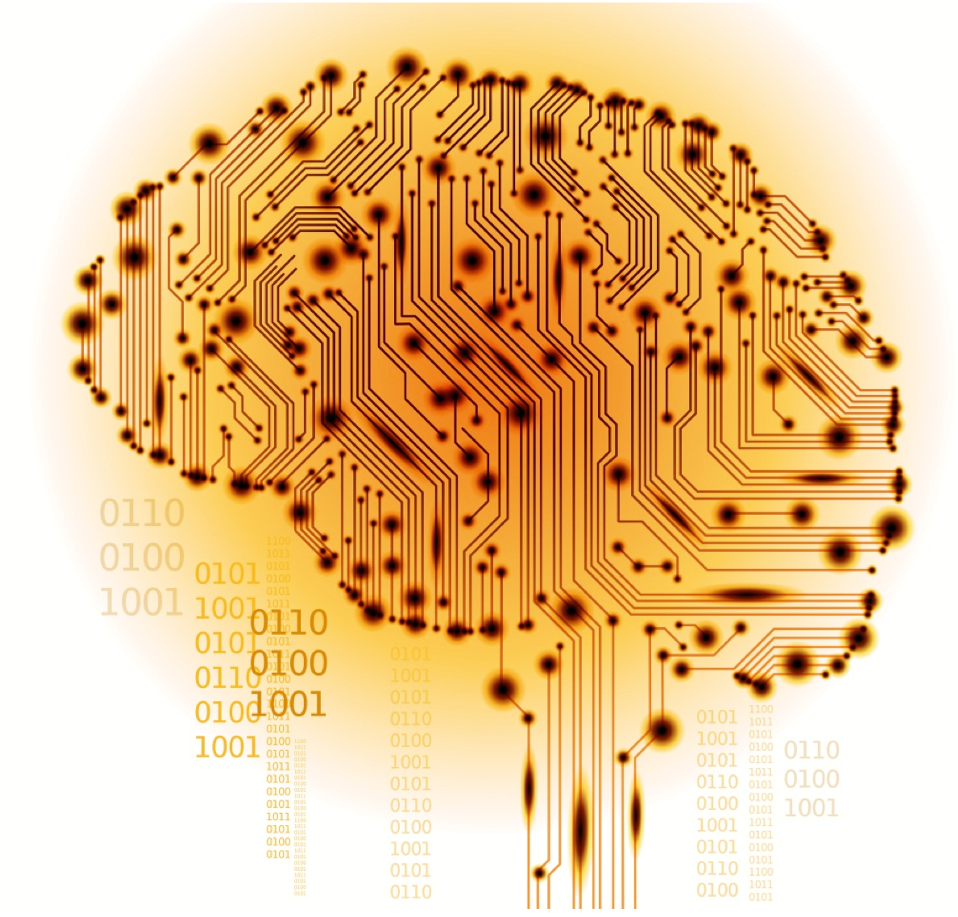
\includegraphics[width=0.95\linewidth]{header/cnn.png}
	\end{minipage}
\end{titlepage}

\setcounter{tocdepth}{2}
\tableofcontents
\newpage

\section{Linear Algebra}

\begin{multicols}{2}
	\subsection{Basic building blocks}
	\textbf{Column} vector ($n\times 1$):
	\[ \bol{x} = \begin{bmatrix} x_1\\x_2\\\vdots\\x_n \end{bmatrix}  \]
	
	\textbf{Row} vector ($1\times n$):
	\[ \bol{x} = \begin{bmatrix} x_1&x_2&\cdots&x_n \end{bmatrix}  \]
	
	Matrix ($3\times 2$):
	\[ \bol{A} = 
	\begin{bmatrix} 
		A_{1,1} & A_{1,2} \\
		A_{2,1} & A_{2,2} \\
		A_{3,1} & A_{3,2}		
	\end{bmatrix}  \]
	
	\subsection{Basic operations}
	\textbf{Transposed} matrix:
	\[ \bol{A}^T = 
	\begin{bmatrix} 
	A_{1,1} & A_{2,1} & A_{3,1} \\
	A_{1,2} & A_{2,2} & A_{3,2}
	\end{bmatrix}  \]
	
	Adding a vector to a matrix (\textbf{Broadcasting}):
	\[ \bol{C} = \bol{A} + \bol{b}, \text{ where } C_{i,j} = A_{i,j} + b_j \]
	
	Matrix product (dot product):
	\[ \bol{C} = \bol{A}\bol{B}, \text{ where } C_{i,j} = \sum_k A_{i,k} B_{k,j} \]
	The resulting dimensions are: $(q\times p)=(q\times k)(k\times p)$
	
	Element-wise (Hadamard) product: 
	\[ \bol{C} = \bol{A} \odot \bol{B}, \text{ where } C_{i,j}=A_{i,j}B_{i,j} \]
	
	\subsection{Solving an equation}
	The inverse Matrix $\bol{A}^{-1}$ is equal to $\bol{A}^T$ if $\bol{A}$ is orthogonal.
	\[ \bol{A}^{-1}\bol{A} = \bol{I}_n \]
	
	Solving $\bol{A}\bol{x}=\bol{b}$:
	\begin{align*}
		\bol{A}\bol{x} &= \bol{b}\\
		\bol{A}^{-1}\bol{A}\bol{x}&=\bol{A}^{-1}\bol{b}\\
		\bol{I}_n\bol{x}&=\bol{A}^{-1}\bol{b}\\
		\bol{x}&=\bol{A}^{-1}\bol{b}\\
	\end{align*}
	If we want this equation to have at most one solution (i.e., $\bol{A}^{-1}$ exists), we require that there are at most $m$ columns. Hence for $\bol{A}^{-1}$ to exist, we require $m=n$, where all the columns are linearly independent.
	\begin{itemize}
		\item This is an invertible (non-singular) square matrix
		\item If a square matrix has linearly independent columns, it is called a singular matrix
	\end{itemize}
	
	\subsection{Norms}
	A norm $L^p$ is a way to measure the length of a vector.
	\[ \lVert \bol{x} \rVert_p = \left( \sum_i \lvert x_i\rvert^p \right)^{\frac{1}{p}} \]
	
	Since the Euclidean norm $L^2$ is the most common norm, it is often written as $\lVert\bol{x}\rVert$
	\[ \lVert\bol{x}\rVert = \sqrt{\lvert x_1 \rvert^2 + \lvert x_2 \rvert^2 + \cdots + \lvert x_n \rvert^2} \]
	
	The squared $L^2$ norm can be conveniently calculated as $\lVert\bol{x}\rVert^2=\bol{x}^T\bol{x}$\\
	
	Close to zero, the squared $L^2$ norm increases very slowly. For algorithms which depend on the difference between zero and almost zero, the $L^1$ norm is used.
	\[ \lVert\bol{x}\rVert_1 = \sum_i \lvert x_i\rvert \]
	
	The so-called $L^0$ \textit{norm} is used to count the number of non-zero elements.\\
	
	The $L^\infty$ norm is also known as the max norm:
	\[ \lVert\bol{x}\rVert_\infty = \underset{i}{\max}\lvert x_i \rvert \]
	
	To measure the size of a matrix, the Frobenius norm is used, which is basically the $L^2$ norm of vectors applied to matrices:
	\[ \lVert \bol{A}\rVert_F = \sqrt{\sum_{i,j} A_{i,j}^2 }  \]
	
	\subsection{Special Kinds of Matrices and Vectors}
	A diagonal matrix is all zero, except in the diagonal:
	\[ D_{i,j} = 0 \text{ for all } i\neq j \]
	
	It is often denoted as $\text{diag}(\bol{v})$. Multiplying becomes quite fast:
	\[ \text{diag}(\bol{v})\bol{x} = \bol{v}\odot \bol{x} \]
	
	Inverting diagonal matrices is only possible, if all diagonal elements are \textbf{non-zero}:
	\[ \text{diag}(\bol{v})^{-1} = \text{diag}\left( \left[ 1/v_1,\dots ,1/v_n \right]^T \right) \]
	
	A symmetric matrix is a matrix that is equal to its transpose: $\bol{A} = \bol{A}^T$\\
	
	An orthogonal matrix is a square matrix whose rows are mutually orthonormal and whose columns are mutually orthonormal:
	\[ \bol{A}^T\bol{A} = \bol{A}\bol{A}^T = \bol{I} \]
	
	\subsection{Eigendecomposition}
	An \textbf{eigenvector} of $\bol{A}$ is a non-zero vector $\bol{v}$ that satisfies the eigen-equation
	\[ \bol{A}\bol{v} = \lambda\bol{v} \]
	The scalar $\lambda$ is the corresponding eigenvalue.
	\[ \det(\bolA - \lambda \bol{I}) = 0 \]
	\[ \lambda_{1,2} = \frac{-b \pm \sqrt{b^2-4ac}}{2a} \]
	Since the eigenvector $\bol{v}$ could be scaled arbitrarily, and the eigen-equation would still hold, we usually scale the eigenvectors to have a length of one (unit vector).\\
	
	Assume that $\bol{A}$ has $n$ linearly independent eigenvectors $\left \{ \bolv^{(1)},\dots,\bolv^{(n)}  \right \} $ and corresponding eigenvalues $ \left \{ \lambda_1,\dots,\lambda_n \right \} $.\\
	Now we can concatenate these eigenvectors to form a matrix $\bol{V} = \left[ \bolv^{(1)},\dots,\bolv^{(n)} \right]$ and concatenate the corresponding eigenvalues to form the vector $\bol{\lambda} = \left[ \lambda_1,\dots,\lambda_n \right]^T$.
	The Eigendecomposition of $\bolA$ is now given by the equation
	\[ \bolA = \bol{V}\diag(\bol{\lambda})\bol{V}^{-1} \]
	
	Every real symmetric matrix can be written using only real eigenvalues
	\[ \bolA = \bol{Q}\bol{\Lambda}\bol{Q}^T \]
	where $\bol{Q}$ is a orthogonal matrix composed of the unit eigenvectors of $\bolA$ and $\bol{\Lambda}$ is a diagonal matrix containing the corresponding eigenvectors in the diagonal. Note that $\bolA$ is singular, if and only if any of the eigenvalues are zero.
	
%	\subsection{Singular Value Decomposition (SVD)}
%	\subsection{Moore-Penrose Pseudoinverse}
	\subsection{Trace Operator}
	The trace operator simply returns the sum of all the diagonal elements in a square matrix:
	\[ \text{Tr}(\bolA) = \sum_i A_{i,i} \]
	Often the trace operator can be used to replace a sum over some squared errors.
	For example, the Frobenius norm can be written as:
	\[ \lVert \bolA \rVert_F = \sqrt{\text{Tr}\left(\bolA\bolA^T\right)} \]
	
	If the shapes of the involved matrixes allow a circular shift, than the trace operator is invariant to this circular shift:
	\[ \text{Tr}(\bolA\bol{B}\bol{C}) = \text{Tr}(\bol{C}\bolA\bol{B}) = \text{Tr}(\bol{B}\bol{C}\bolA) \]
	Note that the result, and even the final shape, of these shifted matrix products are usually not the same, but their traces are.
	Further, the trace is the \textbf{sum of the eigenvalues}.
	
	\subsection{Determinant}
	\begin{itemize}
		\item The determinant $\det(\bolA)$ is equal to the \textbf{product of all the eigenvalues} of the matrix.
		Hence, if there is a zero-valued eigenvalue, the determinant will also be zero. In fact, this will then be a \textbf{singular} matrix, having \textbf{no unique inverse}.
		\item The absolute value of the determinant is a measure how much a space expands due to the multiplication with this matrix
		\begin{itemize}
			\item Hence if the determinant is zero, at least one dimension of the space collapsed
			\item If the determinant is one, than the multiplication is volume preserving
		\end{itemize}
	\end{itemize}
	The determinant of a product of square matrices equals the product of their determinants:
	\[ \det(\bol{A}\bol{B}) = \det(\bolA)\cdot \det(\bol{B})  \]
	Calculation of the determinant of a $(3\times 3)$ matrix:
	\begin{align*}
	&\det \begin{bmatrix} a&b&c\\d&e&f\\g&h&i \end{bmatrix}\\
	&= a\cdot\det \begin{bmatrix} e&f\\h&i \end{bmatrix} -
	   b\cdot\det \begin{bmatrix} d&f\\g&i \end{bmatrix} +
	   c\cdot\det \begin{bmatrix} d&e\\g&h \end{bmatrix}\\
	&= a(ei-fh) - b(di-fg) + c(dh-eg)\\
	&= aei + bfg + cdh - afh - bdi - ceg
	\end{align*}
	
\end{multicols}
\newpage




%\subsection{Fundamentals\buchSeite{690}}
%\begin{multicols}{2}
%\begin{enumerate}[label={\alph*)}]
%\item $\bigcup\limits_{i=1}^{n}R_i=R$
%\item $R_i$ is a connected set, $i=1,2,\dots ,n$
%\item $R_i\bigcap R_j = 0$ for all $i$ and $j, i\neq j$
%\item $Q(R_i)=$ TRUE for $i=1,2,\dots ,n$
%\item $Q(R_i\bigcup R_j)=$ FALSE for any adjacent regions $R_i$ and $R_j$
%\end{enumerate}
%\vfill
%\columnbreak
%\begin{itemize}
%\item The entire spatial region that is occupied by an image is called $R$
%\item Image segmentation is the task of partitioning $R$ into sub-regions $R_i$
%\item $Q()$ is a measure of similarity of a particular property
%\item d) must be true, since it defines the region
%\item e) must be false, since otherwise, the regions should have been merged
%\end{itemize}
%\end{multicols}
%
%Focus on the intensity values
%\begin{itemize}
%\item If there are discontinuities, a new region starts.
%\item If the intensity does not vary much, then this is one region.
%\end{itemize}
%
%\subsection{Point, line and edge detection\buchSeite{692}}
%When the intensity changes abruptly in a local neighborhood, this indicates an edge. It can be a simple point or a line.
%
%\begin{multicols}{2}
%\subsubsection{Background\buchSeite{692}}
%Abrupt local changes can be detected using derivatives.\\
%First order derivative
%\[
%	\frac{\partial f}{\partial x} = f'(x)=f(x+1)-f(x)
%\]
%The second order derivative
%\[
%	\frac{\partial^2f}{\partial x^2}=\frac{\partial f'(x)}{\partial x}=f''(x)=f(x+1)+f(x-1)-2f(x)
%\]
%This can be calculated using a spatial filter.
%\[
%	\begin{bmatrix}
%	w_1, w_2, w_3\\
%	w_4, w_5, w_6\\
%	w_7, w_8, w_9
%	\end{bmatrix}
%\]
%
%\columnbreak
%
%\begin{itemize}
%\item First order in y direction \\ $w_6=1, w_5=-1$
%\item First order in x direction \\ $w_8=1, w_5=-1$
%\item Second order in y direction \\ $w_6=1, w_4=1, w_5=-2$
%\item Second order in x direction \\ $w_8=1, w_2=1, w_5=-2$
%\end{itemize}
%\ \\
%\end{multicols}
%\subsubsection{Detection of Isolated Points\buchSeite{696}}
%The Laplacian combines the second derivatives in both spatial directions. This results in
%\[
%	\nabla^2f(x,y)=f(x+1,y)+f(x-1,y)+f(x,y+1)+f(x,y-1)-4f(x,y)
%\]
%It can be extended to also include the diagonal terms wich results in the following mask
%\[
%	\begin{bmatrix}
%	 1 & 1 & 1\\
%	 1 & -8 & 1\\
%	 1 & 1 & 1
%	\end{bmatrix}
%\]
%The Laplacian is isotropic with respect to $0^\circ$, $45^\circ$, $90^\circ$ and $135^\circ$. \\
%
%Point detection is now achieved by filtering the image with the mask and thresholding this result image $R$.
%\[
%	g(x,y) = 
%	\begin{cases}
%		1 & \text{if } |R(x,y)| \geq T \\
%		0 & \text{otherwise}
%	\end{cases}
%\]
%
%\subsubsection{Line Detection\buchSeite{697}}
%Often, a line of a known direction should be detected. We use special masks for that particular direction
%\begin{figure}[H]
%	\centering
%	\begin{subfigure}[b]{0.2\textwidth}
%		\centering
%		\begin{tikzpicture}
%			\matrix[3x3mask]{
%				-1 & -1 & -1 \\%
%		    	2  & 2  & 2 \\%
%				-1 & -1 & -1\\};
%		\end{tikzpicture}
%		\caption{Horizontal}
%	\end{subfigure}
%	\begin{subfigure}[b]{0.2\textwidth}
%		\centering
%		\begin{tikzpicture}
%			\matrix[3x3mask]{
%				2  & -1 & -1 \\%
%				-1 & 2  & -1 \\%
%				-1 & -1 & 2 \\%
%			};
%		\end{tikzpicture}
%		\caption{$+45^\circ$}
%	\end{subfigure}
%	\begin{subfigure}[b]{0.2\textwidth}
%		\centering
%		\begin{tikzpicture}
%			\matrix[3x3mask]{
%				-1  & 2 & -1 \\%
%				-1 & 2  & -1 \\%
%				-1 & 2 & -1 \\%
%				};
%		\end{tikzpicture}
%		\caption{Vertical}
%	\end{subfigure}
%	\begin{subfigure}[b]{0.2\textwidth}
%		\centering
%		\begin{tikzpicture}
%			\matrix[3x3mask]{
%				-1 & -1 & 2 \\%
%				-1 & 2  & -1 \\%
%				2  & -1 & -1 \\%
%			};
%		\end{tikzpicture}
%		\caption{$-45^\circ$}
%	\end{subfigure}
%	\caption{Line detection masks}
%\end{figure}
%
%\subsubsection{Edge Models}
%The typical intensity profile of an edge is shown in figure \ref{fig:imseg_edgemodels}.
%Note that the derivatives are very sensitive to noise. Usually the image is smoothed (low pass filtered) before
%edge detection.
%
%\newpage
%\subsubsection{Edge localization\buchSeite{706}}
%\begin{multicols}{2}
%The previously shown method generates edge points. The goal is to keep the ones which truly belong to an edge.
%Since first order derivatives are helpful, a nice way of combining the two partial derivatives into one value is the magnitude of the gradient.
%\columnbreak
%\begin{equation}
%\nabla f = \text{grad}(f) = 
%\begin{bmatrix} g_x \\ g_y \end{bmatrix} 
%= \begin{bmatrix} \frac{\partial f}{\partial x} \\[4pt] \frac{\partial f}{\partial y} \end{bmatrix}\notag
%\end{equation}
%\end{multicols}
%The gradient (which is a vector) points into the direction of the greatest rate of change of $f$ at the location $(x,y)$ and is therefore orthogonal to the direction of the edge, which has no change.
%The magnitude of the gradient vector is the value of the rate of change in that direction.
%\begin{figure}[H]
%	\centering
%	\begin{subfigure}[b]{0.2\textwidth}
%		\centering
%		\begin{tikzpicture}
%			\matrix[3x3mask]{
%				-1 & -1 & -1 \\%
%				0  & 0 & 0 \\%
%				1  & 1 & 1 \\%
%			};
%		\end{tikzpicture}
%		\caption{Prewitt}
%	\end{subfigure}
%	\begin{subfigure}[b]{0.2\textwidth}
%		\centering
%		\begin{tikzpicture}
%			\matrix[3x3mask]{
%				-1 & 0 & 1 \\%
%				-1 & 0 & 1 \\%
%				-1 & 0 & 1 \\%
%			};
%		\end{tikzpicture}
%		\caption{Prewitt}
%	\end{subfigure}
%	\begin{subfigure}[b]{0.2\textwidth}
%		\centering
%		\begin{tikzpicture}
%			\matrix[3x3mask]{
%				-1 & -2 & -1 \\%
%				0 & 0 & 0 \\%
%				1 & 2 & 1 \\%
%			};
%		\end{tikzpicture}
%		\caption{Sobel}
%	\end{subfigure}
%	\begin{subfigure}[b]{0.2\textwidth}
%		\centering
%		\begin{tikzpicture}
%			\matrix[3x3mask]{
%				-1 & 0 & 1 \\%
%				-2 & 0 & 2 \\%
%				-1 & 0 & 1 \\%
%			};
%		\end{tikzpicture}
%		\caption{Sobel}
%	\end{subfigure}
%	\caption{Gradient operators: Prewitt and Sobel masks}
%\end{figure}

\newpage
\section{Probability and Information Theory}
\begin{multicols}{2}
	\subsection{Discrete Variables}
	\begin{itemize}
		\item Discrete \textbf{random variables} have a probability mass function (pmf) denoted by $P(x)$.
		\begin{itemize}
			\item Note that probability 0 is not impossible but \textbf{improbable}
			\item Also probability 1 is not certain just 100\% probable
		\end{itemize}
		\item The equation $ \sum_{x\in \bol{x}} P(x)=1$ must be satisfied
	\end{itemize}
	\textbf{Example:} A discrete RV with $k$ different states and uniform distribution.
	A uniform distribution means that every one of the $k$ states is equally likely, resulting in a pmf
	\[ P(\bol{x}=x_i)=\frac{1}{k} \]
	The notation $P(\bol{x}=x_i)$ means that this $P$ is the pmf of the RV $\bol{x}$ and we would like to evaluate it at state/value $x_i$.

	\subsection{Continuous Variables and pdfs}
	Since continuous RVs can take on an infinite number of values on the real number line, we cannot work with pmf.
	We therefore work with the \textbf{probability density function} (pdf).
	$p(x)$ is called the \textbf{likelihood}, not probability.\\

	The probability of $x$ being in an interval $\left[a,b\right]$ is
	\[ \int_a^b p(x)dx = 1 \]
	\textbf{Example:} An RV which is uniformly distributed on an interval $\left[a,b\right]$ of the real numbers.
	Within this interval $\left[a,b\right]$, $p(x)=\frac{1}{b-a}$, and outside of this interval, the function is zero.

	\subsection{Conditional Probability}
	One of the fundamental goals of machine learning is, that we would like to know the probability of one RV, given the knowledge about another one:
	\[ P(\bol{y}=y|\bol{x}=x)=\frac{P(\bol{y}=y,\bol{x}=x)}{P(\bol{x}=x)} \]

	Joint distributions over many RVs can be written as a product over conditional distributions, each being only over one variable:
	\[ P\left(x^{(1)},\dots,x^{(n)}\right) = P(x^{(1)}) \prod_{i=2}^{n} P\left( x^{(i)}|x^{(1)},\dots,x^{(i-1)} \right) \]
	For $n=3$:
	\begin{align*}
	P(a,b,c)
	&= P(a|b,c)P(b,c)\\
	&= P(a|b,c)P(b|c)P(c)
	\end{align*}

	\subsection{Expectation, Variance and Covariance}
	The ecpectation $\mu$ of a function $f()$ of a RV $x$ is the weighted average over the distribution $P(x)$:
	\begin{align*}
	\text{Discrete: }  &\Exp_{x\sim P}\left[f(x)\right] = \sum_x P(x)f(x)\\
	\text{Continuous: }  &\Exp_{x\sim p}\left[f(x)\right] = \int p(x)f(x)dx
	\end{align*}

	The expectation operator $\Exp$ is a linear operator:
	\[ \Exp_x \left[ \alpha f(x) + \beta g(x) \right] = \alpha\Exp_x \left[f(x)\right] + \beta\Exp_x \left[g(x)\right]\]

	The variance $\sigma^2$ measures the expected squared distance of $f(x)$ to its expected value $\Exp\left[f(x)\right]$:
	\begin{align*}
	\var\left( f(x) \right) &= \Exp \left[ \left( f(x) - \Exp \left[ f(x) \right] \right)^2 \right]\\
	&= \Exp \left[ f(x)^2 \right] - \Exp \left[ f(x) \right]^2
	\end{align*}
	For discrete RVs, the variance can be computed with
	\[ \var(X) = \sum_{i=1}^{n} p_i \cdot (x_i-\mu)^2 \]
	If they are all equally likely (uniformly distributed), this equation can be written as
	\[ \var(X) = \frac{1}{n} \sum_{i=1}^{n} (x_i-\mu )^2 \]

	The \textbf{covariance} gives some sense of how much two RVs are linearly related to each other and also the scale of these RVs:
	\[ \cov\left( f(x),g(y) \right) =
	\Exp \left[ \left( f(x) -\Exp \left[ f(x) \right] \right)\left( g(y) -\Exp \left[ g(y) \right] \right) \right] \]

	The \textbf{correlation} is the covariance divided by the standard deviations $\sigma$ of $f(x)$ and $g(y)$ and can only be in the range of $-1$ to $+1$.\\

	The covariance matrix of a random vector $\bol{x}\in \mathbb{R}^n$ is an $n\times n$ matrix, such that
	\[ \cov(\bol{x})_{i,j}=\cov(x_i,x_j) \]
	The diagonal elements of the covariance matrix give the variance:
	\[ \cov(x_i,x_i) = \var(x_i) \]

	\subsection{Bernoulli Distribution}
	Fundamental distribution for a discrete RV that has only two states, usually called $0$ and $1$.
	It has a single parameter $\phi$, which is simply the probability of state $1$.
	\begin{align*}
	P(x=1) &= \phi \\
	P(x=0) &= 1-\phi\\
	P(\bol{x}=x) &= \phi^x(1-\phi)^{1-x}\\
	\Exp_x\left[x\right] &= \phi\\
	\var_x(x) &= \phi(1-\phi)
	\end{align*}

	\subsection{Multinoulli Distribution}
	A distribution over a discrete variable with $k$ different states.
	The parameter is a vector $\bol{p} \in \left[0,1\right]^{k-1}$ (with $k-1$ elements), where each entry $p_i$ is the probability of state $i$.
	The finale states probability $p_k$ is given by $1-\bol{1}^T\bol{p}$.
	Multinoulliis most often used to describe probabilities over a finite number of classes.

	\subsection{Gaussian Distribution}
	Most commonly used distribution over continuous RVs.
	\[ \mathcal{N}(x;\mu,\sigma^2) = \sqrt{\frac{1}{2\pi\sigma^2}}\exp\left(-\frac{1}{2\sigma^2}(x-\mu)^2\right) \]

	Multidimensional Gaussian distribution, where $\Sigma$ is the covariance matrix:
	\[ \mathcal{N}(\bol{x}; \bol{\mu},\bol{\Sigma}) =
	\sqrt{\frac{1}{(2\pi)^n\det(\bol{\Sigma})}}
	\exp \left( -\frac{1}{2} (\bol{x}-\bol{\mu})^T\bol{\Sigma}^{-1}(\bol{x}-\bol{\mu}) \right) \]

	\begin{itemize}
		\item For simplicity the covariance matrix is often assumed to be a diagonal matrix, hence all dimensions of $\bol{x}$ are uncorrelated.
		\item An even simpler model is the isotropic Gaussian distribution since the covariance matrix is simply a scalar times the identity matrix. Hence, the dimensions are not only uncorrelated but also all have the same variance.
	\end{itemize}

	\subsection{Exponential Distribution}
	\[ p(x;\lambda) = \lambda \bol{1}_{x\ge 0} \exp(-\lambda x) \]
	The $\bol{1}_{x\ge 0}()$ function is equal to the unit step, 1 for $x\ge 0$, 0 else.

	\subsection{Laplace Distribution}
	\[ \text{Laplace}(x;\mu,\gamma)=\frac{1}{2\gamma}\exp\left( -\frac{\lvert x-\mu \rvert }{\gamma} \right) \]
	The bigger $\gamma$, the steeper the peak at position $\mu$.

	\subsection{Useful Properties of Common Functions}
	\textbf{Logistic Sigmoid Function:}
	\begin{align*}
	\sigma(z) &= \frac{1}{1+e^{-z}}\\
	\sigma'(z)&= \sigma(z)\left[ 1-\sigma(z) \right]\\
	1-\sigma(z) &= \sigma(-z)
	\end{align*}

	\textbf{Softmax Function:}
	\begin{align*}
	\text{softmax}(\bol{x})_i = \frac{e^{x_i}}{\sum_{j=1}^{n}e^{x_j}}
	\end{align*}

	\textbf{Hyperbolic Tangent:}
	\begin{align*}
	h(z) &= \tanh(z)\\
	h'(z)&= 1-\left[h(z)\right]^2
	\end{align*}

	\textbf{Rectifier Linear Unit (ReLU):}
	\begin{align*}
	h(z) &= \max\left(0,z\right)\\
	h'(z)&= \begin{cases}
	1 & \text{if } z>0\\
	0 & \text{if } z\le 0
	\end{cases}
	\end{align*}

	\textbf{Softplus Function:}
	\begin{align*}
	\zeta(z) &= \log\left(1+\exp(x)\right)\\
	\zeta'(z)&= \sigma(z)\\
	-\zeta(-z) &= \log\left(\sigma(z)\right)\\
	\zeta(z) &= \int_{-\infty}^{x}\sigma(y)dy
	\end{align*}

	\subsection{Bayes' Rule}
	Bayes' rule is used to find $P(x|y)$ from $P(y|x)$ and $P(x)$. This is a common problem since the distribution of the measurements $y$ might be known for each state $x$. But to be able to decide which state to pick, we need the probability of that state $x$, given the particular measurement $y$.
	\begin{align*}
	P(x|y) &= \frac{P(x)P(y|x)}{P(y)}\\
	P(y)   &= \sum_x P(y|x)P(x)
	\end{align*}

	\subsection{Jacobian Matrix}
	\[ \bol{J} =
	\begin{bmatrix} \frac{\partial \bol{f}}{\partial x_1} & \cdots & \frac{\partial \bol{f}}{\partial x_n} \end{bmatrix} =
	\begin{bmatrix}
	\frac{\partial f_1}{\partial x_1} & \cdots & \frac{\partial f_1}{\partial x_n}\\
	\vdots & \ddots & \vdots \\
	\frac{\partial f_m}{\partial x_1} & \cdots & \frac{\partial f_m}{\partial x_n}
	 \end{bmatrix}   \]

	\subsection{Information Theory}
	\begin{itemize}
		\item Likely events should have low information content
		\item Less likely events should have higher information content
		\item Independent events should have additive information
		\begin{itemize}
			\item For example, finding out that a tossed coin has come up as heads twice should convey twice as much information as finding out that a tossed coin has come up as heads once
		\end{itemize}
	\end{itemize}
	\[ I(x) = \log\left(\frac{1}{P(x)}\right) = -\log \left(P(x)\right) \]
	The average of this self-information describes the uncertainty of an entire distribution using the \textbf{Shannon entropy}:
	\[ H(x) = \Exp_{x\sim P}\left[I(x)\right] = -\Exp_{x\sim P}\left[\log P(x)\right] \]

	\begin{figure}[H]
		\centering
		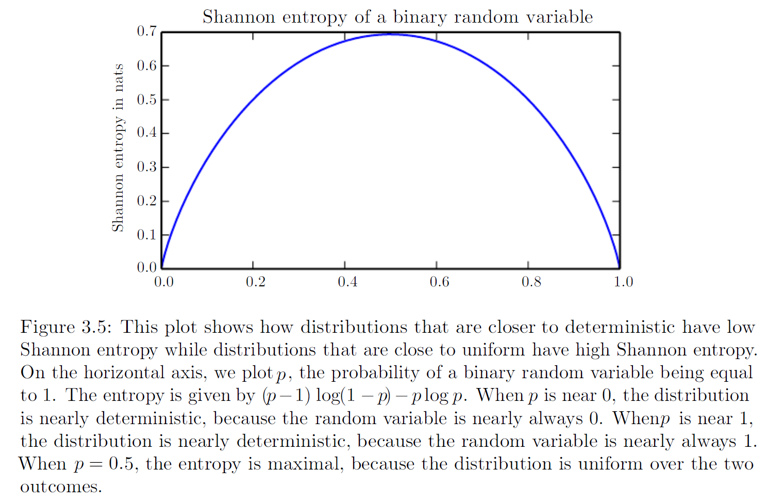
\includegraphics[width=1\linewidth]{images/shannon.png}
	\end{figure}

	\subsection{Kullback-Leibler Divergence}
	The KL divergence can be used to measure how different two distributions P and Q are:
	\[ D_{\text{KL}}(P\lVert Q) = \Exp_{x\sim P}\left[\log \frac{P(x)}{Q(x)}\right]=
	\Exp_{x\sim P}\left[\log {P(x)} \log {Q(x)}\right]
	 \]
	For discrete RVs this is the extra amount of information needed to send a message with symbols drawn from $P$, when the code was designed for $Q$.
	The \textbf{cross entropy} $H(P,Q)$ is the minimum average amount of information needed to transmit symbols drawn from $P(.)$ using a code designed for $Q(.)$:
	\[ H(P,Q) = -\sum_{x} P(x)\log \left(Q(x)\right) \]

	The entropy $H(P)$ is the minimum average amount of information needed to transmit symbols drawn from $P(.)$ using a code designed for $P(.)$:
	\[ H(P) = -\sum_{x} \log\left(P(x)\right) \]

	Hence the KL divergence is the difference DKL $(P\lVert Q)=H(P,Q)-H(P)$:
	\[ -\sum_{x} P(x)\log \left(Q(x)\right) +\sum_{x} \log\left(P(x)\right) \]

	The KL divergence is never negative, and zero if and only if $P$ and $Q$ are the same distributions.

\end{multicols}
\newpage

\section{Numerical Computation}
\begin{multicols}{2}
	\subsection{Overflow and Underflow}
	\textbf{Underflow} occurs when very small numbers are rounded to zero.
	Unfortunately, many functions behave for zero significantly different than for a small positive number, for example $\frac{1}{x}$ and $\log(x)$. In both cases, an overflow will result and further arithmetic will then not result in meaningful results.\\

	\textbf{Overflow} is less common. It occurs when the largest possible internal representation is reached.\\

	For example, the softmax function must be stabilized against under- and overflow:
	\begin{itemize}
		\item Assume that all $x_i$ have the same constant value $c$
		\item This implies that all classes represent the same probability of $1/n$
		\item Hence $1/n$ is the expected result of the softmax$(x)_i$ function, independent of $c$
		\item If the magnitude of $c$ is very large, this might not happen
		\begin{itemize}
			\item[$\rightarrow$] A very negative $c$ leads $e^c$ to underflow, resulting in a $0/0$ problem
			\item[$\rightarrow$] A very positive $c$ leads $e^c$ to overflow, resulting in an $\infty/\infty$ problem
		\end{itemize}
%	\columnbreak
		\item This is achieved by first subtracting the maximum entry of the vector $x$ from the other entries and then calculating the softmax function:
		$$\bol{z}=\bol{x}-\max_ix_i \quad\rightarrow\quad \text{softmax}(\bol{z})$$
		\item To stabilize against underflow which could happen with really small values, we use the log of the softmax:
		\[ \log \text{softmax}(\bol{x}) \]
	\end{itemize}

	\subsection{Gradient-Based Optimization}
	Learning requires a minimization of a loss function. The optimal value minimizing the loss function is often denoted with a superscript $^\ast$:
	\[ \bol{x}^\ast = \arg\,\min f(\bol{x}) \]

	The \textbf{derivative} specifies how a small input change $\epsilon$ results in the corresponding output change:
	\[ f(x+\epsilon) \approx f(x) + \epsilon f'(x) \]

	\textbf{Gradient descent} takes little steps $\epsilon (x\rightarrow x+\epsilon)$ such that $f(x+\epsilon)$ is smaller than $f(x)$.
	Clearly, if $f'(x)=0$, then the derivative provides no information in which direction the function could be minimized.\\

	Usually we need to \textbf{minimize loss functions} depending on a vector.
	Hence we have a scalar function $f(\bol{x})$ depending on many inputs:
	\[ f:\mathbb{R}^n\rightarrow \mathbb{R} \]

	In this case, the partial derivative is used to measure how $f()$ changes as all variables are held constant, except $x_i$ which increases at point $\bol{x}$.
	The \textbf{gradient} generalizes the idea of a derivative in the sense that it represents a derivative of a scalar function with respect to a vector argument $\bol{x}$:
	\[ \nabla_x f(\bol{x}) =
	\begin{bmatrix} \frac{\partial f(\bol{x})}{\partial x_1}\\ \vdots \\ \frac{\partial f(\bol{x})}{\partial x_n} \end{bmatrix}  \]

	The method of \textbf{steepest descent} suggests a new point
	\[ \bol{x}' = \bol{x}-\epsilon\nabla_xf(\bol{x}) \]
	where $\epsilon$ is a small positive scalar and it's called the \textbf{learning rate}.

	\subsection{Jacobian and Hessian Matrices}
	If the function $\bol{f}(\bol{x})$ is a vector valued function of a vector argument $\bol{x}$, then the matrix of all possible partial derivatives is called the \textbf{Jacobian}:
	\[ \bol{f}:\mathbb{R}^m\rightarrow \mathbb{R}^n \qquad \bol{J}\in \mathbb{R}^{n\times m} \]

	Hence the entry $J_{i,j}$ is the partial derivative of the $i^{\text{th}}$ entry of $\bol{f}()$ with respect to the $j^{\text{th}}$ entry of $\bol{x}$:
	\[ J_{i,j} = \frac{\partial}{\partial x_j} f(\bol{x})_i \]

	The second derivative, also called the \textbf{curvature}, is denoted as
	\[ \frac{\partial^2 f}{\partial x_i \partial x_j} \quad\overset{i=j}{\rightarrow}\quad
	\frac{\partial^2 f}{\partial x^2} \]
	If the curvature is zero, then the slope does not change and hence the function is a straight line (1D), a plane (2D) or a hyperplane ($n$D).
	\begin{itemize}
		\item \textbf{Negative} second derivative means, that the slope is getting smaller as the argument gets bigger and hence the function is curving down
		\begin{itemize}
			\item[$\rightarrow$] Hence using the gradient alone, the function value will be overestimated, i.e., the function decreases more than predicted by using the gradient alone
		\end{itemize}
		\item \textbf{Zero} second derivative means, that the slope is constant as the argument gets bigger and hence the function has no curvature
		\begin{itemize}
			\item[$\rightarrow$] Hence using the gradient alone, the function value will be perfectly estimated, i.e., the function decreases as predicted by using the gradient alone
			\item[$\rightarrow$] I.e., for a slope of 1, the function will increase by $\epsilon$ when the argument is increased by $\epsilon$
		\end{itemize}
		\item \textbf{Positive} second derivative means, that the slope is getting larger as the argument gets bigger and hence the function is curving up
		\begin{itemize}
			\item[$\rightarrow$] Hence using the gradient alone, the function value will be underestimated, i.e., the function decreases less than predicted by using the gradient alone
		\end{itemize}
	\end{itemize}

	If the scalar function $f(\bol{x})$ has a vector argument $\bol{x}$, then there are many second derivatives, which are collected together in the \textbf{Hessian}:
	\[ \bol{H}(f)(\bol{x})_{i,j} = \frac{\partial^2 f(\bol{x})}{\partial x_i\partial x_j}
	\quad\rightarrow\quad H_{i,j}=H_{j,i} \]
	Note that the Hessian is nothing else than the Jacobian of the gradient of $f()$.
	Also, the Hessians are \textbf{real and symmetric}, which means they can be decomposed into a set of real eigenvalues and orthogonal eigenvectors.\\

	As in the one-dimensional case, the directional second derivative allows for a prediction how well a gradient descent step will perform. A \textbf{second-order Taylor series approximation} of the function $f(\bol{x})$ around a point $\bol{x}^{(0)}$ is given by the formula
	\[ f(\bol{x}) \approx f(\bol{x}^{(0)}) + \left( \bol{x}-\bol{x}^{(0)} \right)^T\bol{g}+
	\frac{1}{2} \left( \bol{x}-\bol{x}^{(0)} \right)^T\bol{H}\left( \bol{x}-\bol{x}^{(0)} \right) \]

	Given we are at $\bol{x}^{(0)}$ and now we take a small step $\epsilon$ into the direction of the negative gradient $\bol{g}$, then the new point $\bol{x}$ will be given by $\bol{x}=\bol{x}^{(0)}-\epsilon\bol{g}$.
	Now the second order Taylor approximation can be evaluated at this new point $\bol{x}=\bol{x}^{(0)}-\epsilon\bol{g}$:
	\[ f(\bol{x}^{(0)}-\epsilon\bol{g}) \approx f(\bol{x}^{(0)})-\epsilon \bol{g}^T\bol{g}+\frac{1}{2}
	\epsilon^2 \bol{g}^T\bol{H}\bol{g} \]

	\textbf{Newtons method:}
	\begin{align*}
	f(\bol{x}) &\approx f(\bol{x}^{(0)}) + \left( \bol{x}-\bol{x}^{(0)} \right)^T \nabla_x f(\bol{x}^{(0)}) \\
	&+\frac{1}{2} \left( \bol{x}-\bol{x}^{(0)} \right)^T \bol{H}(f)(\bol{x}^{(0)})\left( \bol{x}-\bol{x}^{(0)} \right)
	\end{align*}
	We can now analytically find the minimum of this quadratic function:
	\[ \bol{x}^\ast = \bol{x}^{(0)} - \bol{H}(f)(\bol{x}^{(0)})^{-1}\nabla_x f(\bol{x}^{(0)}) \]

	Problems with Newtons method in deep learning:
	\begin{itemize}
		\item In high dimensions, there are many more saddle points than local minima
		\item Unfortunately Newton’s method will jump to a saddle point and then will be stuck
		\item This is not true for gradient descent
	\end{itemize}

	\subsection{Example: Linear Least Squares}
	In linear least squares, the goal is to find the vector $\bol{x}$ that minimizes the expression
	\[ f(\bol{x}) = \frac{1}{2} \lVert \bol{Ax}-\bol{b}\rVert_2^2 \]
	There are many algorithms to do this, but we will use gradient descent.
	Hence the gradient of this function needs to be calculated:
	\[ \nabla_xf(\bol{x}) =\bol{A}^T (\bol{Ax}-\bol{b}) = \bol{A}^T\bol{Ax}-\bol{A}^T\bol{b} \]
	Now we can follow the negative gradient in little steps to find the minimum:

	\begin{align*}
	\bol{x} &= \bol{x}-\epsilon \nabla_x f(\bol{x})\\
	&= \bol{x} -\epsilon \left(\bol{A}^T\bolA\bol{x}-\bolA^T\bol{b}\right)
	\end{align*}
	These steps are taken as long as the $L^2$ norm of the gradient does not fall below some minimum $\delta$:
	\[ \lVert \bolA^T\bol{Ax}-\bolA^T\bol{b}\rVert_2 > \delta \]


\end{multicols}
\newpage

\section{Machine Learning Basics}
\begin{multicols}{2}
	\subsection{Capacity, Overfitting and Underfitting}
	The goal of machine learning is to perform well on data that has \textbf{never been seen before}.
	Good training results in a low training error while good \textbf{generalization} results in a \textbf{low test error}.
	In linear regression, we train with the training set for a low training error
	\[ \frac{1}{m^{\text{(train)}}} \lVert \bol{X}^{\text{(train)}}\bol{w}-\bol{y}^{\text{(train)}} \rVert_2^2 \]
	but we are really interested in the test error, which we estimate with a test set
	\[ \frac{1}{m^{\text{(test)}}} \lVert \bol{X}^{\text{(test)}}\bol{w}-\bol{y}^{\text{(test)}} \rVert_2^2 \]

	\textbf{Capacity} is loosely defined as the flexibility a model has to fit the data.
	For example, for linear regression the capacity can be increased by allowing \textbf{polynomials} instead of only linear functions:
	\[ \hat{y} = b + wx \quad\rightarrow\quad \hat{y} = b + w_1x + w_2x^2 \]
	The output is still a linear function of the parameter vector $w$, hence the same normal equations derived before can be used to find the solution.
	In other words, we simply pretend that $x^2$ is also an independent input.\\
	The capacity can now simply be controlled by allowing higher and higher orders of polynomials, i.e., for order nine:
	\[ \hat{y} = b + \sum_{i=1}^{9} w_ix^i \]

	In general, machine learning algorithms work best, when their capacity is appropriate in regard to the true complexity of the task they need to perform and the amount of training data they are provided with.
	\begin{figure}[H]
		\centering
		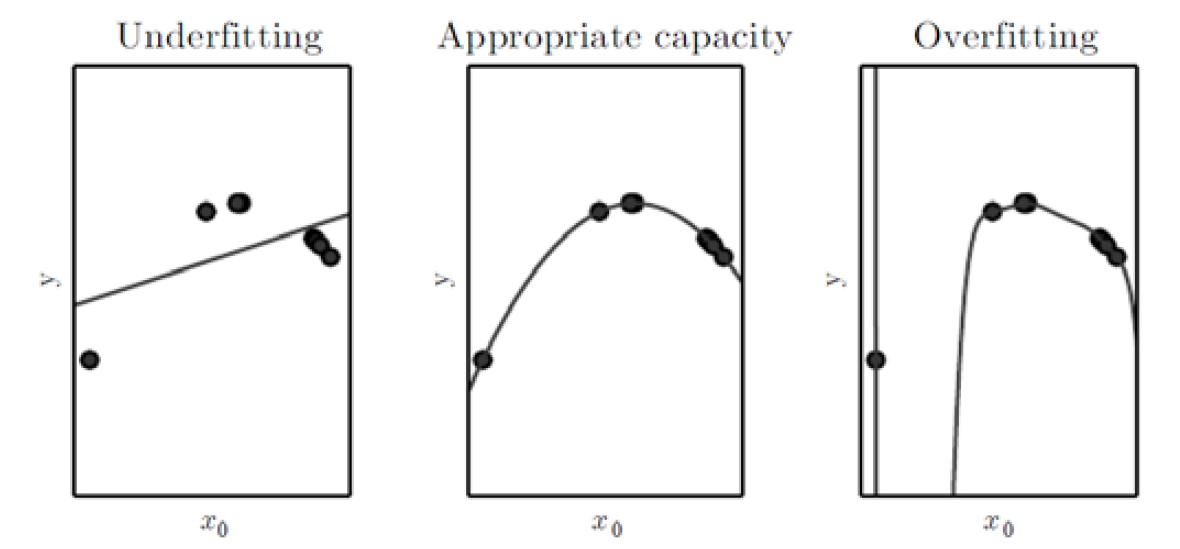
\includegraphics[width=0.85\linewidth]{images/capacity.PNG}
	\end{figure}

	While the training error will only decrease as the capacity is increased, the test error follows a U-shape curve which can be used to find the optimal capacity.
	\begin{figure}[H]
		\centering
		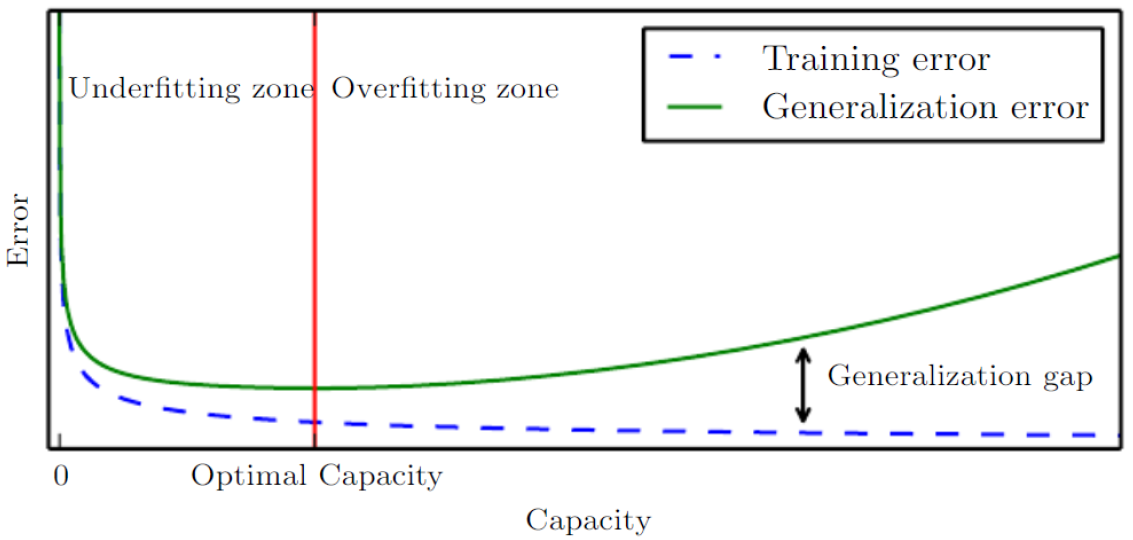
\includegraphics[width=0.95\linewidth]{images/gen_curve.PNG}
	\end{figure}

	The \textbf{ideal model} would know the true data generation distribution and hence could always make the optimal decision or put out the optimal value.
	Nevertheless, in all interesting cases, the test error would not be zero, since the relationship between input $\bol{x}$ and output $y$ might be inherently stochastic or the deterministic output depends on variables that are not in the input.
	The error incurred when having access to the true distribution and making optimal use of it is called the \textbf{Bayes error} or \textbf{irreducible} error and it is the \textbf{smallest possible error}.

	\subsection{Regularization}
	We need to design the machine learning algorithms for the particular task at hand.
	As seen, we can try to match the capacity of the model to the complexity of the task.
	An alternative concept is to steer the algorithm towards preferred solutions.
	For example, in the polynomial regression case, we might be preferring solutions that result in weights that have a small Euclidean norm squared:
	\[ J(\bol{w}) = \text{MSE}_{\text{train}} + \lambda \bol{w}^T\bol{w} \]
	This approach is called weight decay and is quite popular.
	In linear regression this results in the well known \textbf{ridge regression} (\textbf{Tikhonov} regularization).
	If $\lambda$ is zero, then normal linear regression results.
	If $\lambda$ is very large, then the weight vector is basically zero.\\

	\textbf{In general}, a model that is supposed to learn a function $f()$ can be regularized by adding a penalty term called a regularizer to the cost function $f(\bol{x};\bol{\theta})$.
	For weight decay the regularizer is
	\[ \Omega(\bol{w}) = \bol{w}^T\bol{w} \]

	\subsection{Cross-Validation}
	If the available data set is small, then the test set is even smaller, hence estimating the test error is unreliable.
	An approach called \textbf{k-fold cross validation} can then be used to estimate the resulting test error.
	k-fold (k is usually 10) cross validation splits the data into k non-overlapping subsets.
	Then K-1 sets are used to train and the left-out set is used to estimate the test error.
	This is repeated k times and all the test errors of each experiment are averaged.

	\subsection{Bias}
	The bias of an estimator is defined as
	\[ \text{bias}(\hat{\bol{\theta}}_m) = \Exp (\hat{\bol{\theta}}_m)-\bol{\theta} \]
	Estimators are considered unbiased, if the bias is zero, which implies that on average the estimator is correct.
	\[ \Exp (\hat{\bol{\theta}}_m) = \bol{\theta} \]
	A milder form is the idea of asymptotically unbiased, which means as we gather more and more data, the estimator becomes less and less biased, until in the extreme of infinitely many data points it is unbiased
	\[ \underset{m\rightarrow\infty}{\lim} \Exp (\hat{\bol{\theta}}_m) = \bol{\theta} \]

%	\textbf{Example: Bernoulli Distribution:}
%	\[ P(x^{(i)};\theta) = \theta^{x^{(i)}} (1-\theta)^{(1-x^{(i)})} \]
%	The goal of an estimator is to estimate the unknown mean.
%	An obvious estimator would be the average over the training samples:
%	\[ \hat{\theta}_m = \frac{1}{m} \sum_{i=1}^{m} x^{(i)} \]
%
%	\textbf{Example: Gaussian Distribution:}

	\subsection{Variance and Standard Error}
	\textbf{Sample Mean:}
	\[ \hat{\mu}_m = \frac{1}{m} \sum_{i=1}^{m} x^{(i)} \]

	\textbf{Standard Error:}
	\[ \text{SE}(\hat{\mu}_m) = \sqrt{\var\left[\frac{1}{m}\sum_{i=1}^{m}x^{(i)}\right]}
	= \frac{\sigma}{\sqrt{m}} \]

	\textbf{MSE vs. Bias and Variance:}
	\[ \text{MSE} = \Exp\left[(\hat{\theta}_m-\theta)^2\right] = \text{Bias}(\hat{\theta}_m)^2+\var(\hat{\theta}_m) \]


	\subsection{Maximum Likelihood Estimation}
	The idea of the maximum likelihood principle is, that we pick the parameter vector in such a way, that the likelihood that the model would have generated the observed training data is maximized:
	\begin{align*}
	\bol{\theta}_{ML}
	&= \underset{\bol{\theta}}{\arg \max} p_{\text{model}} (\mathbb{X};\bol{\theta})\\
	&= \underset{\bol{\theta}}{\arg \max} \prod_{i=1}^{m} p_{\text{model}} (\bol{x}^{(i)};\bol{\theta})
	\end{align*}

	Usually, the focus is on the \textbf{log likelihood}, since it is simpler:
	\[\bol{\theta}_{ML} = \underset{\bol{\theta}}{\arg \max} \sum_{i=1}^{m} \log p_{\text{model}} (\bol{x}^{(i)};\bol{\theta}) \]

	Note that we can divide the argument in the argmax() operator by $m$, and the result of the argmax operator does not change. But then we have a term where we sum up all the contributions and divide by how many there are:
	\[ \hat{p}_{\text{data}}(\bol{x}) = \frac{1}{m} \sum_{i=1}^{m} \delta(\bol{x}-\bol{x}^{(i)}) \]

	\subsection{Conditional Log-Likelihood and Mean Squared Error}
	In supervised learning we actually need to estimate the conditional probability $P(y|x;\bol{\theta})$.
	If we let $X$ represent all of the input and $Y$ all of the observed targets, then the conditional maximum likelihood estimator is given by
	\[ \bol{\theta}_{ML} = \underset{\bol{\theta}}{\arg \max} P(\bol{Y}|\bol{X};\bol{\theta}) \]

	If (as it is usual) the examples are independent and identically distributed (i.i.d.), then this maximization can be written as
	\[ \bol{\theta}_{ML} = \underset{\bol{\theta}}{\arg \max} \sum_{i=1}^{m} P(\bol{y}^{(i)}|\bol{x}^{(i)};\bol{\theta}) \]

	\textbf{Example: Linear Regression as Maximum Likelihood estimation:}\\
	So far the goal of linear regression was to minimize the MSE.
	For maximum likelihood estimation, we need a parametrized model distribution:
	\[ p(y|\bol{x}) = \mathcal{N}\left(y;\hat{y}(\bol{x};\bol{w}),\sigma^2\right) \qquad
	\hat{y} = \bol{w}^T\bol{x} \]

	Now we use the i.i.d. assumption and hence we can apply the formula
	\[ \bol{\theta}_{ML} = \underset{\bol{\theta}}{\arg \max} \sum_{i=1}^{m} P(\bol{y}^{(i)}|\bol{x}^{(i)};\bol{\theta}) \]

	The log of a Gaussian RV results in several additive terms and the exponent is canceled by the log.
	Hence the following results, where the parameter vector $w$ is now abstracted as parameter vector $\theta$.
	In the formula below, this parameter vector is hidden inside of $\hat{y}$:
	\begin{align*}
	&\sum_{i=1}^{m} \log p\left(y^{(i)}|\bol{x}^{(i)};\bol{\theta}\right)\\
	= &-m\log\sigma - \frac{m}{2}\log(2\pi)-\sum_{i=1}^{m}\frac{\lVert\hat{y}^{(i)}-y^{(i)}\rVert^2}{2\sigma^2}
	\end{align*}

	We need to now pick $\bol{w}$ in such a way, that the equation below is maximized.
	Since the first two terms are independent of $w$, that is equivalent to minimizing the last term.
	Since $\sigma$ is given, this is equal to minimizing the MSE!
	\[ \text{MSE}_{\text{train}}=\frac{1}{m}\sum_{i=1}^{m}\lVert \hat{y}^{(i)}-y^{(i)}\rVert^2 \]

	\subsection{Stochastic Gradient Descent}
	This is a direct extension to gradient descent where the expectation in gradient decent is not calculated over all examples but estimated by \textbf{using only a few sampled} examples.
	The negative conditional log-likelihood of the training data can be written as
	\begin{align*}
	J(\bol{\theta}) &= \Exp_{\bol{x},y\sim \hat{p}_{\text{data}}} L(\vx,y,\bol{\theta})\\
	&= \frac{1}{m} \sum_{i=1}^m L\left(\vx^{(i)},y^{(i)},\bol{\theta}\right)\\
	L\left(\vx,y,\bol{\theta}\right) &= -\log p(y|\vx;\bol{\theta})
	\end{align*}
	$L$ is the per-example loss. Minimizing the negative log likelihood will result in the maximum likelihood solution.
	The log over the i.i.d. samples result in the sum and the division by $m$ is added to make the expression an expectation over the empirical data distribution.\\
	The gradient of this function can be calculated as
	\[ \nabla_{\bol{\theta}}J(\bol{\theta}) = \frac{1}{m}\sum_{i=1}^{m}\nabla_\bolt L\left(\vx^{(i)},y^{(i)},\bolt\right) \]
	Clearly the larger the training set ($m$), the longer a single gradient descent step takes to calculate ($O(m)$).\\

	The main insight of SGD is, that the gradient is an \textbf{expectation}, which can be estimated by using a small set of samples.
	In each step of SGD a so called minibatch of samples is used, where the $m'$ samples are drawn uniformly from the training set $\sB=\{\vx^{(1)},\dots,\vx^{(m')}  \}$. The minibatch size $m'$ ranges between 1 up to maybe 1024 and is \textbf{usually a power of 2}.\\
	Since $m'$ is fixed, the size of the training set $m$ does not matter for the complexity of an SGD step anymore.
	A training set with billions of samples can be trained with minibatches with only hundreds of samples.
	Hence an estimate of the gradient is now formed, using the minibatch samples:
	\[ \bol{g} = \frac{1}{m'} \nabla_\bolt \sum_{i=1}^{m'} L\left(\vx^{(i)},y^{(i)},\bolt\right) \]

	Now this estimate of the gradient is used in the parameter update equation of gradient descent instead of the true gradient
	\[ \bolt \leftarrow \bolt - \epsilon \bol{g} \]

	\subsection{Building a Machine Learning Algorithm}
	Most deep learning algorithms have the same ingredients:
	\begin{itemize}
		\item A large data set
		\item A cost function
		\item A probabilistic model
		\item An optimization algorithm
	\end{itemize}

	\textbf{The cost function} includes almost always a term that causes the learning process to perform some form of statistical estimation.
	Hence the most common cost function is the negative log-likelihood
	\[ J(\bol{w},b) = - \Exp_{\vx,y\sim \hat{p}_{\text{data}}} \log p_{\text{model}}(y|\vx) \]
	Minimizing the negative log-likelihood results in a maximum likelihood estimation.\\

	The cost function often contains additional regularization terms, for example, the weight decay term we have already seen for linear regression:
	\[ J(\bol{w},b) = \lambda\lVert \bol{w}\rVert_2^2 - \Exp_{\vx,y\sim \hat{p}_{\text{data}}} \log p_{\text{model}}(y|\vx) \]
	This implies that \textbf{weights closer to zero are preferred} over larger weights.
	In linear regression the addition of this term does still result in a closed form solution, the well known ridge regression.

	\subsection{Local Constancy and Smoothness Regularization}
	For algorithms to generalize well, they need to be guided by some form of prior knowledge about the problem, especially in the high-dimensional case, this is of fundamental importance.
	A very popular prior belief is the smoothness (local constancy) prior
	\[ f^\ast (\vx) \approx f^\ast (\vx + \epsilon) \]
	Basically, the function we try to learn should not change very much in a small neighborhood $\epsilon$.
	Many classical machine learning schemes are based on this (KNN, Trees, SVM) and as a result, they tend to fail in more complex tasks.
	Deep learning introduces additional priors in order to reduce the generalization error on more challenging tasks.\\
	Classical learning algorithms need $O(k)$ examples to distinguish $O(k)$ regions in the input space using a smoothness prior.\\

	The smoothness assumption works well in low dimensions, if there are enough training points.
	In high dimensions, the function might still be smooth, but it can change simultaneously in many dimensions.
	In addition it might behave differently in different regions.
	The function might also be quite complicated, i.e., there is a large number of regions compared to the number of examples. Is it possible to generalize in these cases?\\

	The answer is Yes, as long as we introduce some dependencies between the regions.
	For example, if we can use 2 training examples ($X_1$ and $X_2$) to define $2^2=4$ regions, if we assume a structure as shown below:
	\begin{table}[H]
		\centering
		\begin{tabular}{c|c|c|}
			& $X_1$ & NOT $X_1$ \\
			\hline
			$X_2$ & Region 1 & Region 2 \\
			\hline
			NOT $X_2$ & Region 3 & Region 4 \\
			\hline
		\end{tabular}
	\end{table}

	Hence this is achieved via additional assumptions about the underlying data generating distribution.
	Many deep learning algorithms provide implicit or explicit assumptions that are reasonable for a broad range of AI tasks in order to capture these advantages.
	These assumptions are much more sophisticated than the simple relationship shown in the table.\\

	Traditional machine learning algorithms often make stronger, task specific assumptions.
	For the checkerboard example, assuming some form of periodicity would clearly improve the generalization, but is very specific.
	In deep learning, such strong task specific assumptions are avoided, hence they often are widely applicable.
	Complex AI tasks have a much too complex structure, as that they could be captured with simple ideas like periodicity.\\

	\textbf{Composition of factors} is the core idea of deep learning, we assume that the data was generated hierarchically over several levels by the composition of factors.
	These mild assumptions allow for an exponential gain in the relationship between the number of training examples and the number of regions that can be distinguished.
	\begin{figure}[H]
		\centering
		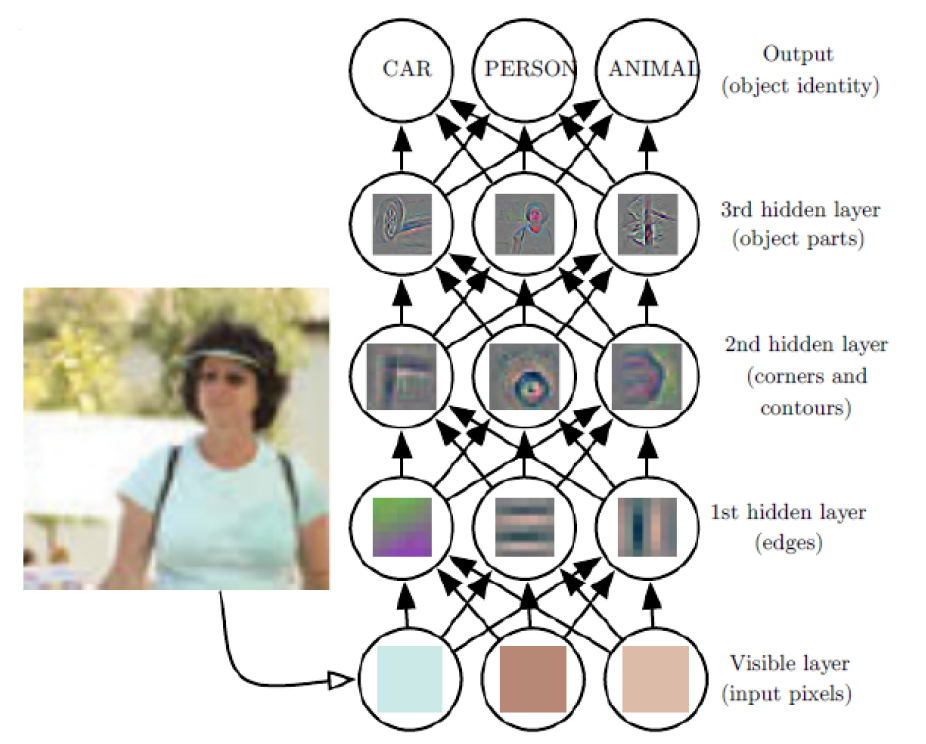
\includegraphics[width=0.75\linewidth]{images/whut.PNG}
	\end{figure}

	\subsection{Manifold Learning}
	A manifold is a set of points associated with a neighborhood around each point.
	From any given point, the manifold locally appears to be a Euclidean space.
	For example, we experience the surface of the world as a 2D plane but it is actually a 2D spherical manifold in 3D.
	The idea of a manifold is, that the connected set of points can be approximated well by considering only a small number of degrees of freedom, or dimensions, embedded in a higher-dimensional space. Each dimension corresponds to a local direction of variation as can be seen in the figure below.
	\begin{figure}[H]
		\centering
		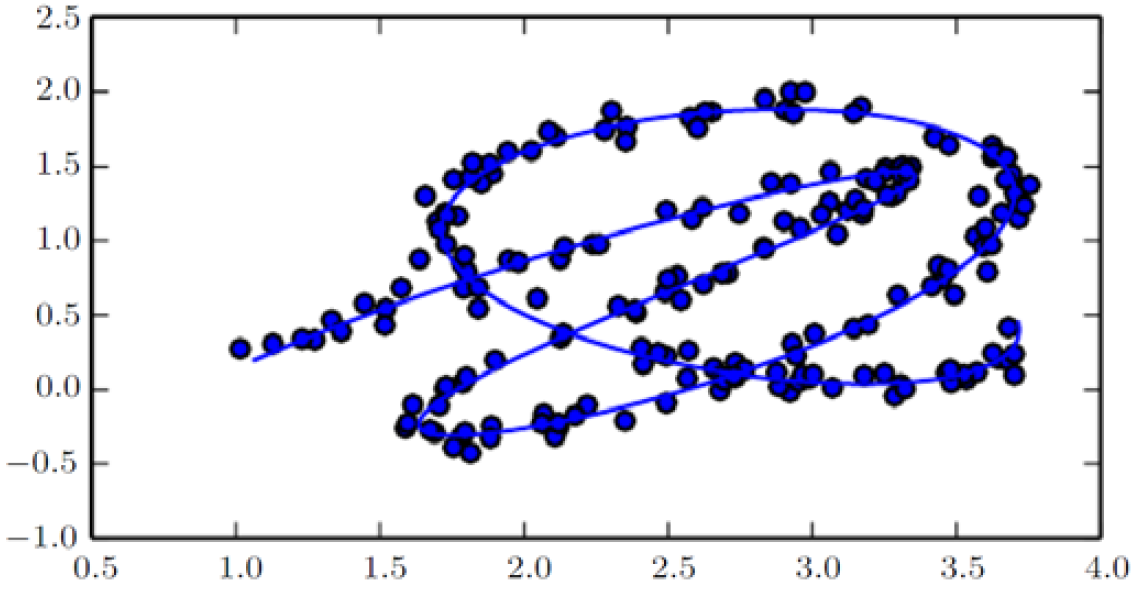
\includegraphics[width=0.75\linewidth]{images/mani.PNG}
	\end{figure}
	Now one can move from point to point along a manifold. Clearly the hope is, that these points are training samples.
	In machine learning, the dimensionality of the manifold is allowed to vary from one point to another.
	This happens for example, when the manifold has a self intersection.
	A figure \textbf{8} has a one dimensional manifold at all points, except at the intersection, where it clearly has two dimensions.
	Many problems seem arbitrarily complex, if the scheme needs to learn functions with interesting variations across all dimensions.
	In manifold learning, this is simplified by assuming that interesting inputs must lie along manifolds. Hence most inputs are not valid inputs.\\

	The assumption that the data lies along a low-dimensional manifold may not always be correct or useful.
	For complex AI tasks, such as computer vision, speech recognition and/or natural language processing, it appears that this manifold assumption is at least approximately correct.
	One piece of evidence, that the manifold assumption is useful for describing the probability distribution over images, text and sound, is the fact that uniform noise never resembles structured inputs from this domain.\\

	When the data lies on a low-dimensional manifold then it can be most natural to represent the data in terms of the coordinates of this manifold.
	For example roads are 1D manifolds in a 3D world. Addresses in the 3D world are naturally given with respect to the 1D manifold we call road and not in 3D coordinates. Explicitly extracting these manifold coordinates is challenging, but hold the promise to improve many machine learning algorithms.
\end{multicols}
\newpage

\section{Deep Feedforward Networks}
\begin{multicols}{2}
	\subsection{Chain Rule}
	\textbf{Scalar chain rule:}
	\[ \frac{\partial z}{\partial x} = \frac{\partial z}{\partial y} \frac{\partial y}{\partial x} \]

	If $\bol{y}=g(\bol{x})$ and $z = f(\bol{y})$, then (\textbf{Vector chain rule}):
	\[ \frac{\partial z}{\partial x_i} = \sum_j \frac{\partial z}{\partial y_j} \frac{\partial y_j}{\partial x_i} \]

	In vector notation, this may be equivalently written as
	\[ \nabla_x z = \left( \frac{\partial \bol{y}}{\partial \bol{x}} \right)^T \nabla_y z
	= \sum_{j=1}^{m}(\nabla_xy_j) \frac{\partial z}{\partial y_j} \]

	\textbf{Tensor chain rule:}
	\[ \nabla_{\bm{\mathsf{x}}} z = \sum_j (\nabla_{\bm{\mathsf{x}}} \bol{Y}_j )\frac{\partial z}{\partial \bol{Y}_j} \]



	\subsection{Output Units\buch{Chapter 6.2.2}\buchSeite{180}}
	The choice of cost function is tightly coupled with the choice of output unit. Most	of the time, we simply use the cross-entropy between the data distribution and the	model distribution. The choice of how to represent the output then determines the form of the cross-entropy function.\\

	\subsubsection{Linear Units for Gaussian Output Distributions}
	One simple kind of output unit is an output unit based on an affine transformation with no nonlinearity. These are often just called linear units.
	Given features $\vh$, a layer of linear output units produces a vector $\hat{y} = \mW ^\top \vh + b$.\\
	Maximizing the log-likelihood is then equivalent to minimizing the mean squared	error.


	\subsubsection{Sigmoid Units for Bernoulli Output Distributions}
	Sigmoid units are the standard output units for binary output variables.
	The use of the maximum likelihood approach is to define a Bernoulli distribution over $y$ conditioned on $\bol{x}$:
	\[ P(y=1|\bol{x}) \]
	A Bernoulli distribution is defined by the probability of the event occurring, which can be stated as
	\[ P(y=1|\bol{x}) = \max \left\{ 0,\min \left\{ 1, \bol{w}^T\bol{h}+b \right\} \right\} \]
	While this hard limited linear function results in a valid conditional distribution, gradient descent could not train this efficiently, since the slope is zero for large and small values.
	The \textbf{sigmoid function} is a form of a soft limited linear function and hence the slope does never become exactly zero, though at large values it does become quite small:
	\[ \hat{y} = \sigma \left(\bol{w}^T\bol{h}+b\right) \]


	\subsubsection{Softmax Units for Multinoulli Output Distributions}
	Any time we wish to represent a probability distribution over a discrete variable with n possible values, we may use the softmax function. This can be seen as a	generalization of the sigmoid function which was used to represent a probability distribution over a binary variable.\\
	In the case of binary variables, we wished to produce a single number
	\[ \hat{y} = P(y = 1 \mid \textbf{x})\]

	To generalize to the case of a discrete variable with n values, we now need	to produce a vector $\hat{\vy}$, with $\hat{\vy_{i}} = P(y = i \mid \textbf{x})$. We require not only that each element of $\hat{\vy}$ be between 0 and 1, but also that the entire vector sums to 1 so that it represents a valid probability distribution.\\
	First, a linear	layer predicts unnormalized log probabilities:
	\[ \vz =  \mW^\top \vh + \vb\]

	where $z_{i} = \log\tilde{P}(y = i \mid x)$. The softmax function can then exponentiate and	normalize $\vz$ to obtain the desired $\hat{\vy}$. Formally, the softmax function is given by
	\[ \softmax(\vz)_{i} = \frac{\exp(\vz_{i})}{\sum \exp(\vz_{j})} \]

	As with the logistic sigmoid, the use of the exp function works very well when training the softmax to output a target value y using maximum log-likelihood. In this case, we wish to maximize $\log P(y = i; z) = \log \softmax(z)_i$. Defining the softmax in terms of exp is natural because the log in the log-likelihood can undo the exp of the softmax:

	\[ \log \softmax(\vz)_{i} = z_{i} - log\sum_{j}\exp(\vz_{j}) \]


	\subsubsection{Other Output Types\buch{chapter 6.2.2.4}\buchSeite{182}}
	\newpage
\end{multicols}
%\begin{figure}[H]
%	\centering
%	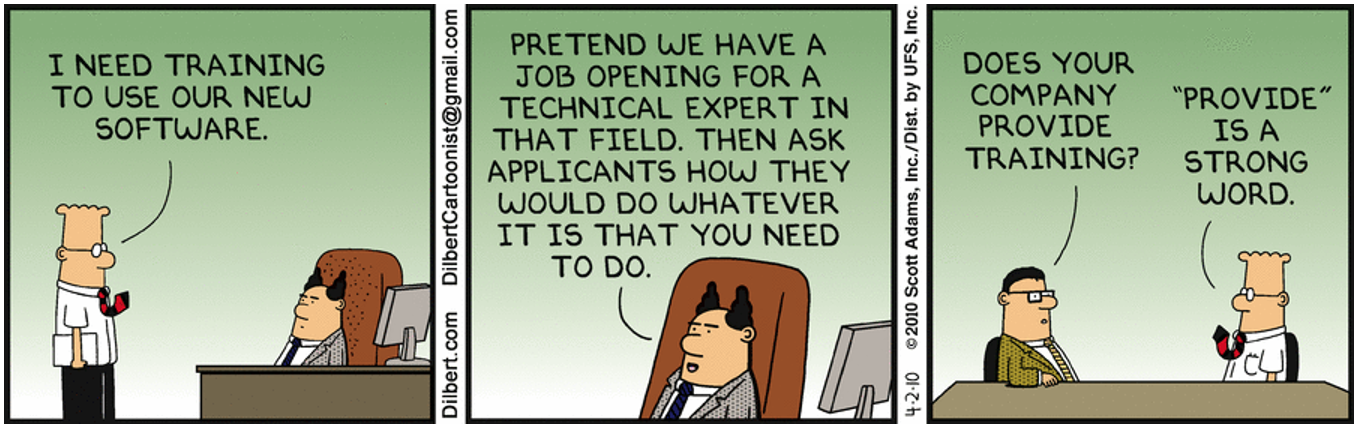
\includegraphics[width=0.65\linewidth]{images/comic.PNG}
%\end{figure}

\section{Regularization for Deep Learning}
\begin{multicols}{2}
	A goal of machine learning is, that the algorithm generalizes, that is, that it will perform well on data it has never been trained with.
	Regularization is any strategy that is designed to reduce the test error, often at the expense of increasing the training error.

	\subsection{Parameter Norm Penalties}
	Many regularization approaches are based on limiting the capacity of models by adding a parameter norm penalty to the objective function as
	\[ \tilde{J}(\bolt;\mX,\vy) = J(\bolt;\mX,\vy)+\alpha\Omega(\bolt) \]
	Here $\alpha$ is a nonnegative hyperparameter that weights the contribution of the norm penalty.\\

	Note that in deep learning, the biases (which are part of the parameter set) are usually not part of the norm penalty, since this can introduce a significant amount of underfitting. Hence only the weight matrices are usually regularized using a norm penalty. So instead of using $\bolt$, the vector $\vw$ (containing all the weights) is now used in the norm penalty function.

	\subsection{$L^2$ Parameter Regularization}
	When the Euclidean norm is used for the penalty, than a scheme called weight decay results.
	Note this scheme is also called ridge regression or Tikhonov regularization.
	\[ \Omega(\bolt) = \frac{1}{2} \lVert \vw \rVert_2^2 \]

	It is now clear what happens at a single step, the weights decay towards zero:
	\[ \vw \leftarrow (1-\epsilon\alpha)\vw-\epsilon\nabla_\vw J(\vw;\mX,\vy) \]

	A quadratic approximation to the unregularized objective function $J$ in the neighborhood of the value of the weights $\vw^\ast$ that obtains minimal unregularized cost $J$ is employed
	\[ \vw^\ast = \argmin_\vw J(\vw) \]

	This approximation is given by the expression
	\[ \hat{J}(\bolt) = J(\vw^\ast)+\half(\vw-\vw^\ast)^T\mH(\vw-\vw^\ast) \]
	$\mH$ is the Hessian of $J$ with respect to $\vw$ evaluated at $\vw^\ast$, and is positive semidefinite.
	Clearly the minimum of this approximation occurs where its gradient is zero (since this is a quadratic function), which is at $\vw^\ast$
	\[ \nabla_\vw \hat{J}(\vw)=\mH(\vw-\vw^\ast) \]

	Now the weight decay gradient is added to the gradient of the unregularized cost $J$, resulting in the gradient of the regularized cost and setting it to zero to find the minimum $\tilde{\vw}$ of the regularized cost.
	\begin{align*}
	\nabla_\vw \tilde{J}(\vw;\mX,\vy)
	&= \alpha\vw + \overbrace{\nabla_\vw J(\vw;\mX,\vy)}^{\nabla_\vw\hat{J}(\vw)=\mH(\vw-\vw^\ast)}\\
	\alpha\tilde{\vw}+\mH(\tilde{\vw}-\vw^\ast) &= 0\\
	(\mH+\alpha\mI)\tilde{\vw} &= \mH\vw^\ast\\
	\tilde{\vw}&=(\mH+\alpha\mI)^{-1}\mH\vw^\ast
	\end{align*}
	The final line shows, that if $\alpha$ approaches zero, the regularized solution $\tilde{\vw}$ approaches $\vw^\ast$, the unregularized minimum.\\
	What happens if $\alpha$ grows? Since $\mH$ is real and symmetric, it can be decomposed into a diagonal matrix and an orthonormal basis of eigenvectors as
	\[ \mH = \mQ\bol{\Lambda}\mQ^T \]

	Hence we can apply this decomposition and the following equation results
	\begin{align*}
	\tilde{\vw}	&= (\mH+\alpha\mI)^{-1}\mH\vw^\ast\\
	&= (\mQ\bol{\Lambda}\mQ^T+\alpha\mI)^{-1}\mQ\bol{\Lambda}\mQ^T\vw^\ast\\
	&=\left[\mQ(\bol{\Lambda}+\alpha\mI)\mQ^T\right]^{-1}\mQ\bol{\Lambda}\mQ^T\vw^\ast\\
	&= \mQ(\bol{\Lambda}+\alpha\mI)^{-1}\bol{\Lambda}\mQ^T\vw^\ast
	\end{align*}
	Multiplying from the left with $\mQ^T$ results in the following relationship between $\mQ^T\tilde{\vw}$ and $\mQ^T\vw^\ast$:
	\[ \left[\mQ^T\tilde{\vw}\right] =(\bol{\Lambda}+\alpha\mI)^{-1}\bol{\Lambda}\left[\mQ^T\vw^\ast\right] \]
	Consider the vector $\left[\mQ^T\vw^\ast\right]$, which is $\vw^\ast$ expressed in terms of the eigenvectors.\\
	Consider the vector $\left[\mQ^T\tilde{\vw}\right]$, which is $\tilde{\vw}$ expressed in terms of the eigenvectors.\\
	The matrix $(\bol{\Lambda}+\alpha\mI)^{-1}\bol{\Lambda}$ is a diagonal matrix with the diagonal elements
	\[ \frac{\lambda_i}{\lambda_i+\alpha} \]
	Hence, the component of $\vw^\ast$ that is aligned with the $i^{\text{th}}$ eigenvector of $\mH$ is rescaled by the factor $\lambda_i/(\lambda_i+\alpha)$.\\

	Along the directions where the eigenvalues of $\mH$ are relatively large, the effect of regularization is relatively small.
	However, components with small $\lambda$s, will be shrunk to have nearly zero magnitude.
	Only directions along which the parameters contribute significantly to reducing the unregularized $J$ are preserved relatively intact. In directions that do not contribute to reducing the unregularized $J$, a small eigenvalue of the Hessian tells us that movement in this direction will not significantly increase the gradient.\\

	Now this analysis is applied to linear regression.
	Note that in linear regression, the true cost function is quadratic and hence the approximation used so far fits the model perfectly
	\[ \hat{y} = \mX\vw \]
	The corresponding optimal solution is
	\[ \vw = (\mX^T\mX)^{-1}\mX^T\vy \]
	Now the $L^2$ regularization term is added, resulting in the new objective function
	\[ (\mX\vw-\vy)^T(\mX\vw-\vy)+\half\alpha\vw^T\vw \]
	and the corresponding optimal solution is
	\[ \vw = (\mX^T\mX+\alpha\mI)^{-1}\mX^T\vy \]
	Note that $\mX^T\mX$ is proportional to the covariance matrix $(\mX^T\mX)/m$.
	$L^2$ regularization replaces $\mX^T\mX$ with $(\mX^T\mX+\alpha\mI)$, hence the same matrix but with an additional $\alpha$ term added to the diagonal elements.

	\subsection{$L^1$ Regularization}
	An alternative is $L^1$ regularization where the penalty term is defined as
	\[ \Omega(\bolt) = \lVert\vw\rVert_1 = \sum_i \lvert w_i\rvert \]

	The regularized objective function now becomes
	\[ \tilde{J}(\vw;\mX,\vy) = \alpha\lVert\vw\rVert_1+j(\vw;\mX,\vy) \]

	This results in the following gradient w.r.t. the weights $\vw$
	\[ \nabla_\vw \tilde{J}(\vw;\mX,\vy)=\alpha \sign(\vw)+\nabla_\vw J(\mX,\vy;\vw) \]
	Note the sign function is applied elementwise, i.e., results in a vector filled with +1 or -1.\\
	$L^1$ regularization is clearly quite different. The contribution of the regularization to the gradient no longer scales linearly with each $w_i$, instead it is a constant factor $\alpha$ with the sign equal to the sign of $w_i$.\\

	The problem of minimizing this approximate cost function has an analytical solution (for each dimension $i$), with the following form:
	\begin{align*}
	\tilde{\hat{J}}(\vw;\mX,\vy)
	&= J(\vw^\ast;\mX,\vy)+\sum_i\left[\half H_{i,i}(\vw_i-\vw_i^\ast)^2+\alpha\lvert w_i\rvert\right]\\
	w_i &= \sign(w_i^\ast)\max\left\{ \lvert w_i^\ast\rvert-\frac{\alpha}{H_{i,i}},0 \right\}
	\end{align*}

	The graph below shows that $L^1$ results in more zero weights than $L^2$, hence $L^1$ regularization results in a sparser solution. $L^2$ does not encourage zero explicitly but only favors smaller values.
	\begin{figure}[H]
		\centering
		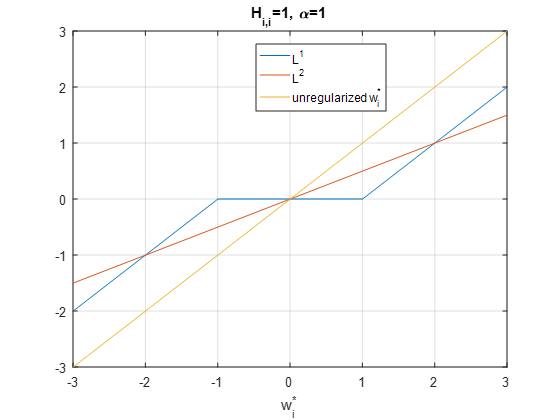
\includegraphics[width=0.9\linewidth]{images/L1L2.png}
	\end{figure}

	\subsection{Early Stopping}
	When the model has sufficient capacity to overfit, then the learning curves should look like the one below:
	\begin{figure}[H]
		\centering
		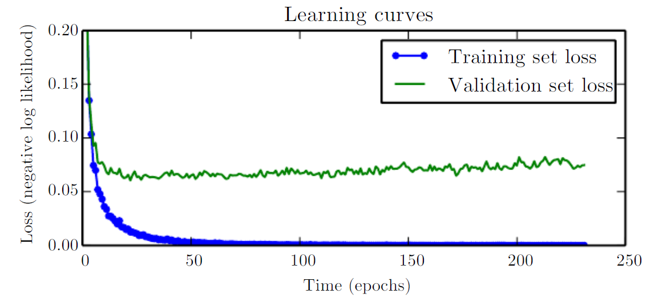
\includegraphics[width=0.9\linewidth]{images/earlystopping.png}
	\end{figure}
	Hence the model after 200 epochs is worse at the validation data set than after 30 epochs, so the model at 30 epochs should be used, since a better validation error should also result in a better test error.\\

	Early stopping is an unobtrusive form of regularization, in that it requires almost no change in the underlying training procedure, the objective function, or the set of allowable parameter values.
	This means that it is easy to use early stopping without damaging the learning dynamics.
	This is \textbf{in contrast to weight decay}, where one must be careful not to use too much weight decay and trap the network in a bad local minimum corresponding to a solution with pathologically small weights.\\

	Early stopping requires a validation set, hence some labeled data is not used for training.
	There are three basic approaches how this data can be used for training the model:
	\begin{enumerate}
		\item Don’t do it, just have enough data
		\item Expensive idea: once early stopping has figured out the optimal number of training epochs, reset everything and train for this optimal number of iterations using all data
		\begin{itemize}
			\item[$\rightarrow$] Usually not done in practice, where the training sets are large and the training takes a long time
		\end{itemize}
		\item Less expensive idea, but a bit tricky: Basically after the stopping criterion has been reached, keep training, now using all the data
	\end{enumerate}
	How does early stopping act as a regularizer?\\
	\vdots\\
	Under the given assumptions, the number of training iterations $\tau$ plays a role inversely proportional to the $L^2$ regularization parameter $\alpha$:
	\[ \alpha \approx \frac{1}{\tau\epsilon} \]
	\begin{figure}[H]
		\centering
		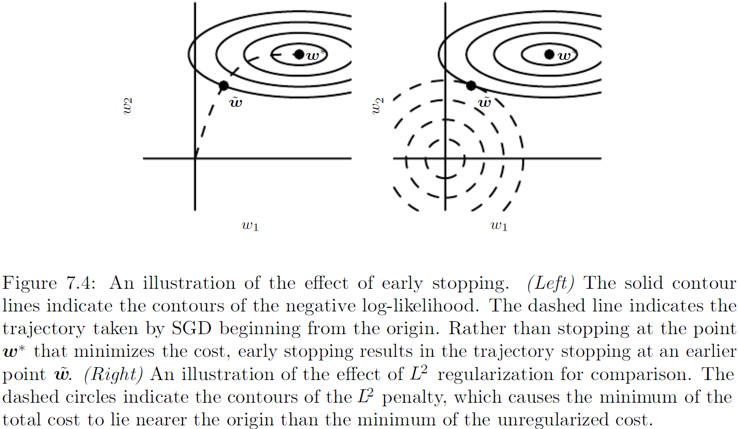
\includegraphics[width=1\linewidth]{images/earlyvsl2.png}
	\end{figure}
	As we have shown before, parameter values corresponding to directions of significant curvature (of the objective function) are regularized less than directions of less curvature. Of course, in the context of early stopping, this really means that parameters that correspond to directions of significant curvature tend to be learned \textbf{early} relative to parameters corresponding to directions of less curvature.
		\subsection{Dataset Augmentation}
	The best way to make a machine learning model generalize better, is to train it on more data. Dataset augmentation is directly applicable for classification, where a mapping between some high dimensional input \textbf{x} and a single category y needs to be learned.
	A few approaches for object recognition:
	\begin{itemize}
		\item Random Cropping
		\item Random color shift
		\item Noise injection
	\end{itemize}
	Dataset Augementation has also been very successful in speech recognition.
	\begin{figure}[H]
		\centering
		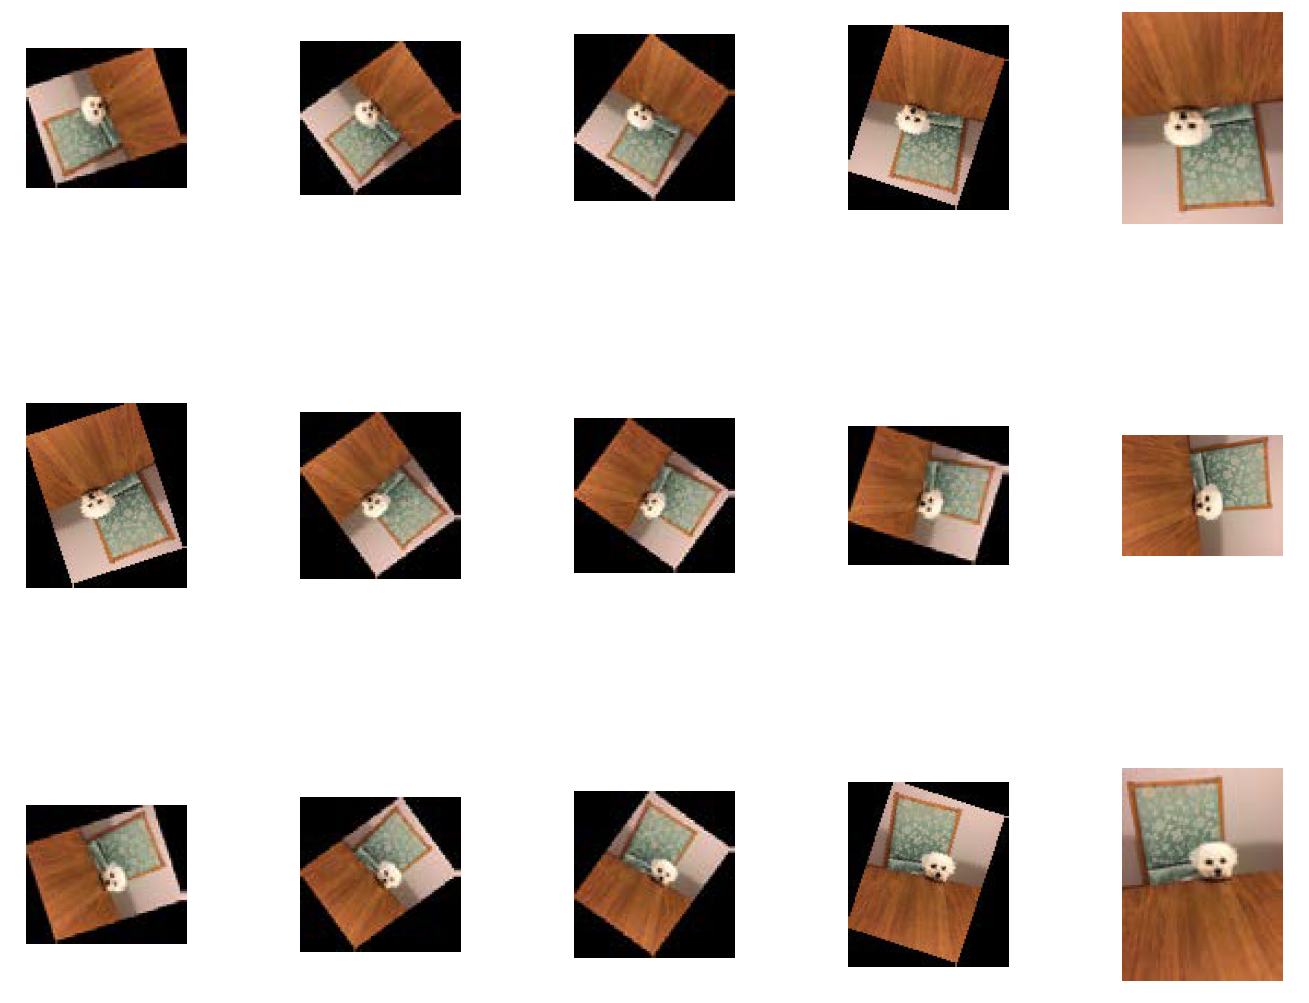
\includegraphics[width=1\linewidth]{images/datasetAugementation.PNG}
	\end{figure}

	\subsection{Bagging and other Ensemble Methods}
	The idea is to train several different models separately, then have all of the models vote on the output for test examples.
	This is an example of a general strategy in machine learning called model averaging. Techniques employing this strategy are known as \textbf{ensemble methods}.
	The main reason why this works is, that different models will make different, and \emph{ideally, uncorrelated}, errors. Hence averaging the model responses will reduce the variance of the errors:
	\begin{align*}
	\E\left[\left(\frac{1}{k}\sum_i\epsilon_i\right)^2\right]
	&= \frac{1}{k^2}\E\left[\sum_i\left(\epsilon_i^2+\sum_{j\neq i}\epsilon_i\epsilon_j\right)\right]\\
	&= \frac{1}{k}v+\frac{k-1}{k}c
	\end{align*}
	The formula clearly shows, that for perfectly correlated errors $(c=v)$, averaging the predictions and hence averaging the errors does not help.
	In the case the errors are completely \textbf{uncorrelated} $c=0$, the well known result is achieved, that the error variance $v$ is reduced by the number of models $k$.
	Hence in the \textbf{worst case} it is not worse than a single model.
	In the \textbf{best case} it is better by a factor $k$. This assumes that the mean error is zero.\\

	\textbf{Bootstrap aggregating (bagging)} is a method that allows the same kind of model, training algorithm and objective function to be reused several times.
	Bagging involves constructing $k$ different datasets. Each dataset has the same number of examples as the original dataset, but each dataset is constructed by sampling with replacement from the original dataset.\\
	This means that, with high probability, each dataset is missing some of the examples from the original dataset and also contains several duplicate examples (on average around $2/3$ of the examples from the original dataset are found in the resulting training set, if it has the same size as the original).\\
	Model $i$ is then trained on dataset $i$. The differences between which examples are included in each dataset result in differences between the trained models.
	\begin{figure}[H]
		\centering
		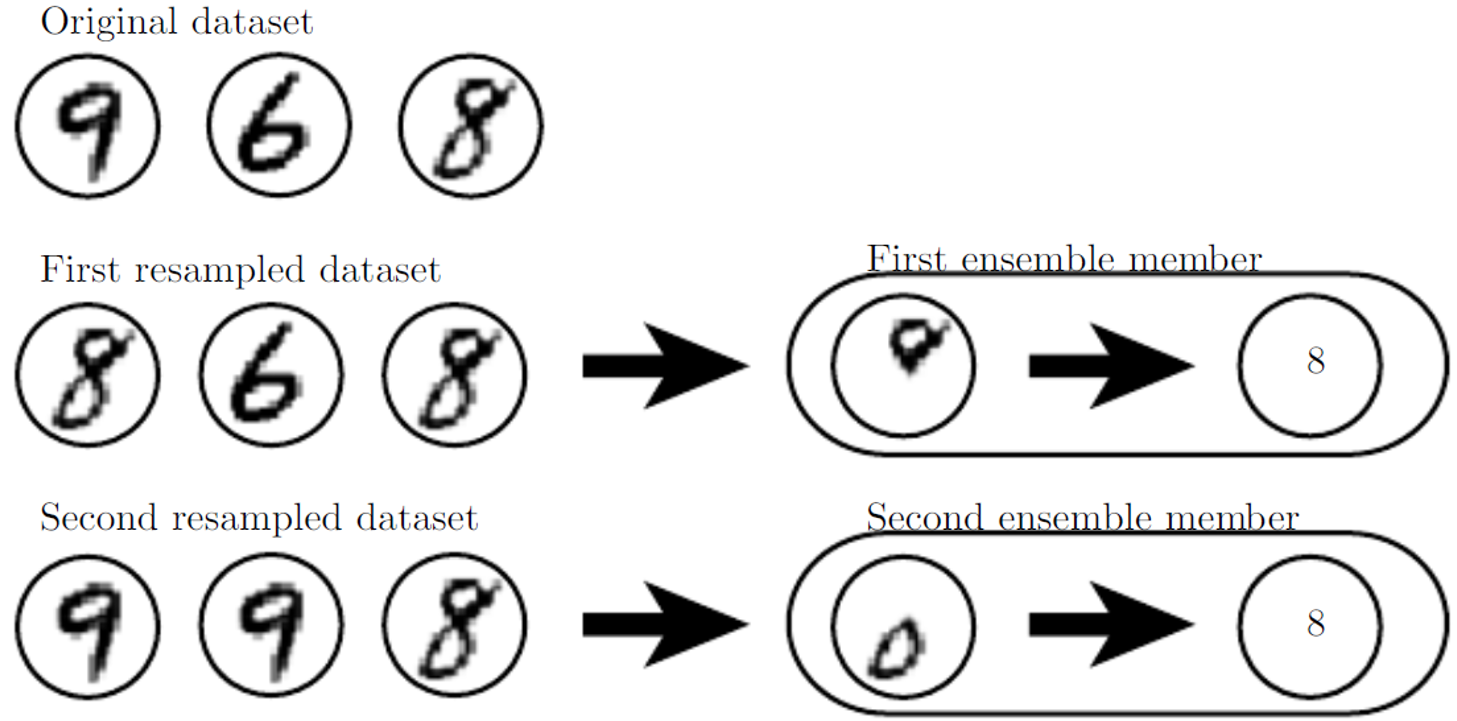
\includegraphics[width=0.85\linewidth]{images/bagging.PNG}
	\end{figure}
	Differences in random initialization, random selection of minibatches, differences in hyperparameters, or different outcomes of non-deterministic implementations of neural networks are often enough to cause different members of the ensemble to make partially independent errors.

	\subsection{Noise Robustness \& Dropout}
	Dropout provides a computationally inexpensive but powerful method of regularizing a broad family of models.
	Dropout can be thought of as a method of making bagging practical for ensembles of very many large neural networks.
	Bagging involves training multiple models, and evaluating multiple models on each test example.
	This seems \textbf{impractical} when each model is a \textbf{large neural network}, since training and evaluating such networks is \textbf{costly in terms of runtime and memory}.\\

	Dropout trains the ensemble consisting of all sub-networks that can be formed by \textbf{removing non-output units} from an underlying base network.
	In the example below, there are 4 non-output units, each can either be part of the network or not. Hence there are $2^4=16$ possible configurations.
	\begin{figure}[H]
		\centering
		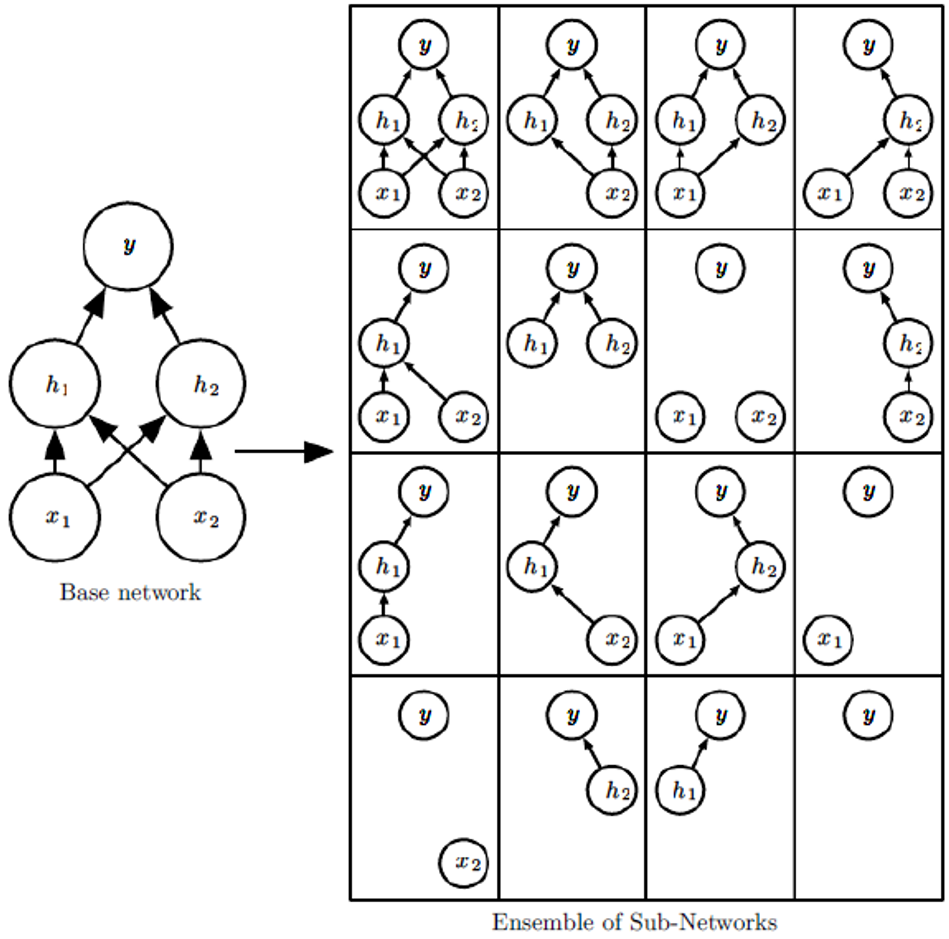
\includegraphics[width=0.9\linewidth]{images/dropoutensemble.png}
	\end{figure}
	In most modern neural networks, based on a series of affine transformations and nonlinearities, we can effectively remove a unit from a network by \textbf{multiplying its output value by zero}.
	Each time we load an example into a minibatch, we randomly sample a different binary mask to apply to all of the input and hidden units in the network. The mask for each unit is sampled independently from all of the others.\\

	The \textbf{probability of sampling a mask value} of one (causing a unit to be included) is a \textbf{hyperparameter fixed before training begins}. It is not a function of the current value of the model parameters or the input example.
	Typically, an input unit is included with probability 0.8 and a hidden unit is included with probability 0.5. We then run forward propagation, back-propagation, and the learning update as usual.\\

	In the case of bagging, the models are all independent. In the case of dropout, the models \textbf{share parameters}, with each model inheriting a different subset of parameters from the parent neural network.
	This parameter sharing makes it possible to represent an exponential number of models with a tractable amount of memory.\\

	In the case of bagging, each model is trained to convergence on its respective training set.
	In the case of dropout, typically most models are not explicitly trained at all—usually, the model is large enough that it would be infeasible to sample all possible subnetworks. Instead, a tiny fraction of the possible sub-networks are each trained for a single step (minibatch), and the parameter sharing causes the remaining sub-networks to arrive at good settings of the parameters.\\

	These are the only differences. Beyond these, dropout follows the bagging algorithm. For example, the training set encountered by each sub-network is indeed a subset of the original training set sampled with replacement, i.e., a minibatch.\\

	Now, we assume that the model's role is to output a probability distribution.
	In the case of bagging, each model $i$ produces a probability distribution $ p^{(i)}(y|\vx) $.
	The prediction of the ensemble is given by the arithmetic mean of all of these distributions:
	\[ \frac{1}{k}\sum_{i=1}^{k}p^{(i)}(y|\vx) \]
	In the case of dropout, each sub-model defined by mask vector $\vmu$ defines a probability distribution.
	The arithmetic mean over all masks is given by
	\[ \sum_\vmu p(\vmu)p(y|\vx,\vmu) \]
	where $p(\vmu)$ is the probability distribution that was used to sample $\vmu$ at training time.

	There is plenty of evidence that the \textbf{geometric mean} performs comparably to the arithmetic mean in this context.
	To guarantee that the result is a probability distribution, we impose the requirement that none of the sub-models assigns probability 0 to any event, and we re-normalize the resulting distribution.
	The unnormalized probability distribution defined directly by the geometric mean is given by
	\[ \tilde{p}_{\text{ensemble}}(y|\vx) = \sqrt[2^d]{\prod_\vmu p(y|\vx,\vmu)} \]

	To make predictions we must re-normalize the ensemble:
	\[ p_{\text{ensemble}}(y|\vx) = \frac{\tilde{p}_{\text{ensemble}}(y|\vx)}{\sum_{y'}\tilde{p}_{\text{ensemble}}(y'|\vx)} \]
	Amazingly, we can approximate this distribution $p_{\text{ensemble}}(y|\vx)$ by evaluating $p(y|\vx)$ in \textbf{one} model.
	The motivation for this modification is to capture the right expected value of the output from that unit.
	Because we usually use an inclusion probability of 0.5, this rule basically amounts to \textbf{dividing the weights by 2} at the end of training, and then using the model as usual.
	The goal is to make sure that the expected total input to a unit at test time is roughly the same as the expected total input to that unit at train time, even though half the units at train time are missing on average.\\

	For many classes of models that do not have nonlinear hidden units, this rule is exact.
	For a simple example, consider a softmax regression classifier with $n$ input variables represented by the $n$-dimensional vector $\vv$:
	\[ P(\ry=y|\vv) =\softmax\left(\mW^T\vv+\vb\right)_y \]

	We can index into the family of sub-models by element-wise multiplication of the input with a binary vector $\vd$:
	\[ P(\ry=y|\vv;\vd) = \softmax\left(\mW^T(\vd\odot\vv)+\vb\right)_y \]

	The ensemble predictor is defined by re-normalizing the geometric mean over all ensemble members predictions
	\[ \tilde{P}_{\text{ensemble}}(\ry=y|\vv) = \sqrt[2^n]{\prod_{\vd\in\{0,1\}^n} P(\ry=y|\vv;\vd)} \]

	Again, the assumption is, that each element of the vector $\vd$ has a probability of 0.5 to be either 0 or 1. Hence this uniform distribution simplifies the presentation, since $p(\vd)$ is a constant and hence will cancel out
	\[ P_{\text{ensemble}}(\ry=y|\vv) = \frac{\tilde{P}_{\text{ensemble}}(\ry=y|\vv)} {\sum_{y'}\tilde{P}_{\text{ensemble}}(\ry=y'|\vv)} \]

	\textbf{Dropout is computationally cheap}: Using dropout during training requires only $O(n)$ computation per example per update, to generate $n$ random binary numbers and multiply them by the state.
	Running inference in the trained model has the same cost per-example as if dropout were not used, though we must pay the cost of dividing the weights by 2 once before beginning to run inference on examples.\\

	For very large datasets, regularization confers little reduction in generalization error.
	In these cases, the computational cost of using dropout and larger models may outweigh the benefit of regularization.\\

	The \textbf{power of dropout} arises from the fact that the masking noise is applied to the hidden units.
	This can be seen as a form of highly intelligent, adaptive destruction of the information content of the input rather than destruction of the raw values of the input.\\
	For \textbf{example}, if the model learns a hidden unit that detects a face by finding the nose, then dropping this unit corresponds to erasing the information that there is a nose in the image.
	The model must learn another hidden unit, either that redundantly encodes the presence of a nose, or that detects the face by another feature, such as the mouth.
	Destroying extracted features rather than original values allows the destruction process to make use of all of the knowledge about the input distribution that the model has acquired so far.

%	\subsection{Bagging and other Ensemble Methods}
%	The idea is to train several different models separately, then have all of the models vote on the output for test examples.
%	This is an example of a general strategy in machine learning called model averaging. Techniques employing this strategy are known as \textbf{ensemble methods}.
%	The main reason why this works is, that different models will make different, and \emph{ideally, uncorrelated}, errors. Hence averaging the model responses will reduce the variance of the errors:
%	\begin{align*}
%	\E\left[\left(\frac{1}{k}\sum_i\epsilon_i\right)^2\right]
%	&= \frac{1}{k^2}\E\left[\sum_i\left(\epsilon_i^2+\sum_{j\neq i}\epsilon_i\epsilon_j\right)\right]\\
%	&= \frac{1}{k}v+\frac{k-1}{k}c
%	\end{align*}
%	The formula clearly shows, that for perfectly correlated errors $(c=v)$, averaging the predictions and hence averaging the errors does not help.
%	In the case the errors are completely \textbf{uncorrelated} $c=0$, the well known result is achieved, that the error variance $v$ is reduced by the number of models $k$.
%	Hence in the \textbf{worst case} it is not worse than a single model.
%	In the \textbf{best case} it is better by a factor $k$. This assumes that the mean error is zero.\\
%
%	\textbf{Bootstrap aggregating (bagging)} is a method that allows the same kind of model, training algorithm and objective function to be reused several times.
%	Bagging involves constructing $k$ different datasets. Each dataset has the same number of examples as the original dataset, but each dataset is constructed by sampling with replacement from the original dataset.\\
%	This means that, with high probability, each dataset is missing some of the examples from the original dataset and also contains several duplicate examples (on average around $2/3$ of the examples from the original dataset are found in the resulting training set, if it has the same size as the original).\\
%	Model $i$ is then trained on dataset $i$. The differences between which examples are included in each dataset result in differences between the trained models.
%	\begin{figure}[H]
%		\centering
%		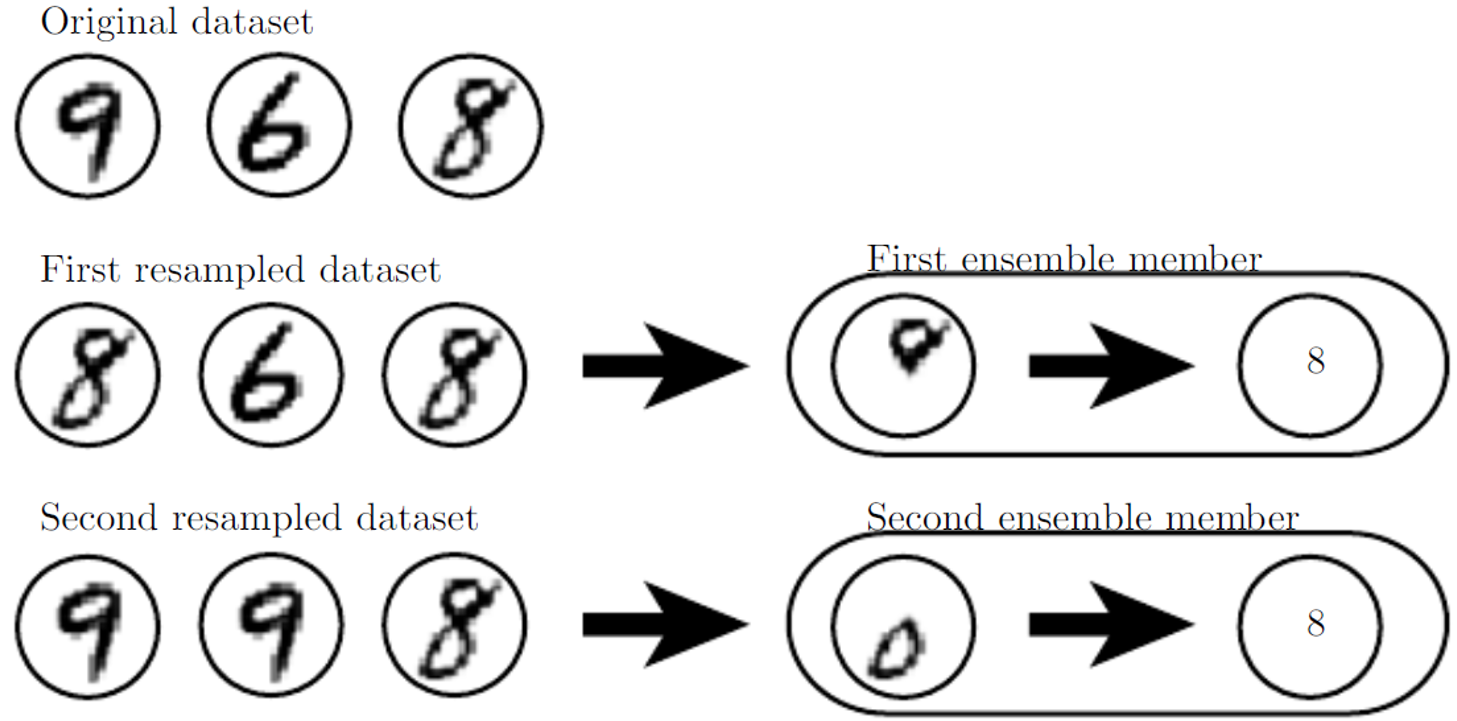
\includegraphics[width=0.85\linewidth]{images/bagging.PNG}
%	\end{figure}
%	Differences in random initialization, random selection of minibatches, differences in hyperparameters, or different outcomes of non-deterministic implementations of neural networks are often enough to cause different members of the ensemble to make partially independent errors.
%
%	\subsection{Dropout}
%	Dropout provides a computationally inexpensive but powerful method of regularizing a broad family of models.
%	Dropout can be thought of as a method of making bagging practical for ensembles of very many large neural networks.
%	Bagging involves training multiple models, and evaluating multiple models on each test example.
%	This seems \textbf{impractical} when each model is a \textbf{large neural network}, since training and evaluating such networks is \textbf{costly in terms of runtime and memory}.\\
%
%	Dropout trains the ensemble consisting of all sub-networks that can be formed by \textbf{removing non-output units} from an underlying base network.
%	In the example below, there are 4 non-output units, each can either be part of the network or not. Hence there are $2^4=16$ possible configurations.
%	\begin{figure}[H]
%		\centering
%		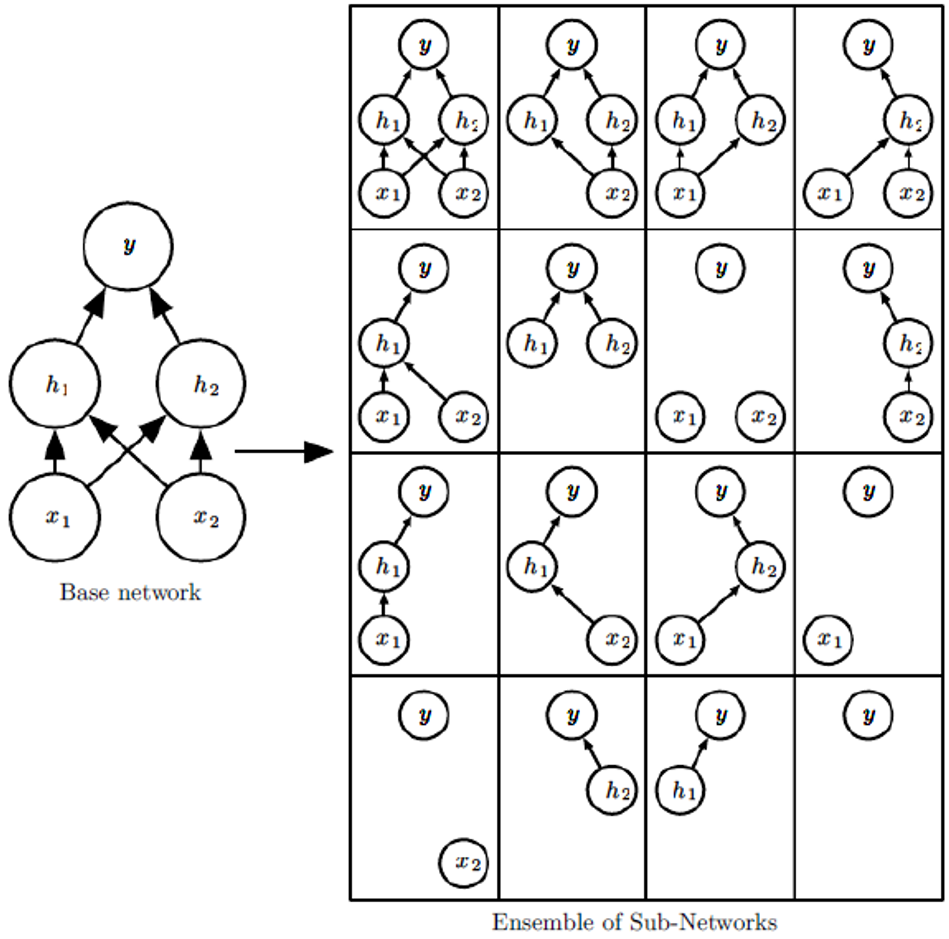
\includegraphics[width=0.9\linewidth]{images/dropoutensemble.png}
%	\end{figure}
%	In most modern neural networks, based on a series of affine transformations and nonlinearities, we can effectively remove a unit from a network by \textbf{multiplying its output value by zero}.
%	Each time we load an example into a minibatch, we randomly sample a different binary mask to apply to all of the input and hidden units in the network. The mask for each unit is sampled independently from all of the others.\\
%
%	The \textbf{probability of sampling a mask value} of one (causing a unit to be included) is a \textbf{hyperparameter fixed before training begins}. It is not a function of the current value of the model parameters or the input example.
%	Typically, an input unit is included with probability 0.8 and a hidden unit is included with probability 0.5. We then run forward propagation, back-propagation, and the learning update as usual.\\
%
%	In the case of bagging, the models are all independent. In the case of dropout, the models \textbf{share parameters}, with each model inheriting a different subset of parameters from the parent neural network.
%	This parameter sharing makes it possible to represent an exponential number of models with a tractable amount of memory.\\
%
%	In the case of bagging, each model is trained to convergence on its respective training set.
%	In the case of dropout, typically most models are not explicitly trained at all—usually, the model is large enough that it would be infeasible to sample all possible subnetworks. Instead, a tiny fraction of the possible sub-networks are each trained for a single step (minibatch), and the parameter sharing causes the remaining sub-networks to arrive at good settings of the parameters.\\
%
%	These are the only differences. Beyond these, dropout follows the bagging algorithm. For example, the training set encountered by each sub-network is indeed a subset of the original training set sampled with replacement, i.e., a minibatch.\\
%
%	Now, we assume that the models role is to output a probability distribution.
%	In the case of bagging, each model $i$ produces a probability distribution
%	The prediction of the ensemble is given by the arithmetic mean of all of these distributions:
%	\[ \frac{1}{k}\sum_{i=1}^{k}p^{(i)}(y|\vx) \]
%	In the case of dropout, each sub-model defined by mask vector $\vmu$ defines a probability distribution.
%	The arithmetic mean over all masks is given by
%	\[ \sum_\vmu p(\vmu)P(y|\vx,\vmu) \]
%	where $p(\vmu)$ is the probability distribution that was used to sample $\vmu$ at training time.
%
%	There is plenty of evidence that the \textbf{geometric mean} performs comparably to the arithmetic mean in this context.
%	To guarantee that the result is a probability distribution, we impose the requirement that none of the sub-models assigns probability 0 to any event, and we renormalize the resulting distribution.
%	The unnormalized probability distribution defined directly by the geometric mean is given by
%	\[ \tilde{p}_{\text{ensemble}}(y|\vx) = \sqrt[2^d]{\prod_\vmu p(y|\vx,\vmu)} \]
%
%	To make predictions we must re-normalize the ensemble:
%	\[ p_{\text{ensemble}}(y|\vx) = \frac{\tilde{p}_{\text{ensemble}}(y|\vx)}{\sum_{y'}\tilde{p}_{\text{ensemble}}(y'|\vx)} \]
%	Amazingly we can approximate this distribution $p_{\text{ensemble}}(y|\vx)$ by evaluating $p(y|\vx)$ in \textbf{one} model.
%	The motivation for this modification is to capture the right expected value of the output from that unit.
%	Because we usually use an inclusion probability of 0.5, this rule basically amounts to \textbf{dividing the weights by 2} at the end of training, and then using the model as usual.
%	The goal is to make sure that the expected total input to a unit at test time is roughly the same as the expected total input to that unit at train time, even though half the units at train time are missing on average.\\
%
%	For many classes of models that do not have nonlinear hidden units, this rule is exact.
%	For a simple example, consider a softmax regression classifier with $n$ input variables represented by the $n$-dimensional vector $\vv$:
%	\[ P(\ry=y|\vv) =\softmax\left(\mW^T\vv+\vb\right)_y \]
%
%	We can index into the family of sub-models by element-wise multiplication of the input with a binary vector $\vd$:
%	\[ P(\ry=y|\vv;\vd) = \softmax\left(\mW^T(\vd\odot\vv)+\vb\right)_y \]
%
%	The ensemble predictor is defined by re-normalizing the geometric mean over all ensemble members predictions
%	\[ \tilde{P}_{\text{ensemble}}(\ry=y|\vv) = \sqrt[2^n]{\prod_{\vd\in\{0,1\}^n} P(\ry=y|\vv;\vd)} \]
%
%	Again, the assumption is, that each element of the vector $\vd$ has a probability of 0.5 to be either 0 or 1. Hence this uniform distribution simplifies the presentation, since $p(\vd)$ is a constant and hence will cancel out
%	\[ P_{\text{ensemble}}(\ry=y|\vv) = \frac{\tilde{P}_{\text{ensemble}}(\ry=y|\vv)} {\sum_{y'}\tilde{P}_{\text{ensemble}}(\ry=y'|\vv)} \]
%
%	\textbf{Dropout is computationally cheap}: Using dropout during training requires only $O(n)$ computation per example per update, to generate $n$ random binary numbers and multiply them by the state.
%	Running inference in the trained model has the same cost per-example as if dropout were not used, though we must pay the cost of dividing the weights by 2 once before beginning to run inference on examples.\\
%
%	For very large datasets, regularization confers little reduction in generalization error.
%	In these cases, the computational cost of using dropout and larger models may outweigh the benefit of regularization.\\
%
%	The \textbf{power of dropout} arises from the fact that the masking noise is applied to the hidden units.
%	This can be seen as a form of highly intelligent, adaptive destruction of the information content of the input rather than destruction of the raw values of the input.\\
%	For \textbf{example}, if the model learns a hidden unit that detects a face by finding the nose, then dropping this unit corresponds to erasing the information that there is a nose in the image.
%	The model must learn another hidden unit, either that redundantly encodes the presence of a nose, or that detects the face by another feature, such as the mouth.
%	Destroying extracted features rather than original values allows the destruction process to make use of all of the knowledge about the input distribution that the model has acquired so far.

\end{multicols}
\newpage

\section{Optimization for Training Deep Models}
\begin{multicols}{2}
	\subsection{Batch and Minibatch Algorithms}
	Note that maximum likelihood estimation problems, when viewed in log space, decompose into a sum over each example
	since i.i.d. samples result in a likelihood consisting of the product of all samples.
	\[\bol{\theta}_{ML} = \underset{\bol{\theta}}{\arg \max} \sum_{i=1}^{m} \log p_{\text{model}} (\bol{x}^{(i)},y^{(i)};\bol{\theta}) \]
	Maximizing this sum is equivalent to maximizing the expectation over the empirical distribution defined by the training set.
	\[ J(\bolt) = \Exp_{\vx,y\sim \hat{p}_{\text{data}}} \log p_{\text{model}}(\vx,y;\bolt) \]
	This expectation is simply the sample mean over the $m$ training samples. The division by $m$ is a constant factor hence it does not change the optimal value for $\bolt$.
	Most of the properties of the objective function $J$ used by most of our optimization algorithms are expectations over the training set.\\

	Optimization algorithms that use the \textbf{entire training set} are called \textbf{batch} or \textbf{deterministic gradient} methods, because they process all of the training examples simultaneously in a large batch.\\

	Optimization algorithms that use only a \textbf{single example} at a time are called \textbf{stochastic methods}.\\

	Most algorithms used for deep learning fall somewhere in between, using more than one but less than all of the training examples.
	These were traditionally called minibatch or minibatch stochastic methods and it is now common to simply call them stochastic methods.\\

	It is \textbf{crucial} that the minibatches are \textbf{selected randomly}.
	Computing an unbiased estimate of the expected gradient from a set of samples requires that those samples be independent.
	We also wish for two subsequent gradient estimates to be independent from each other, so two subsequent minibatches of examples should also be independent from each other.
	Furthermore, in cases where the order of the dataset holds some significance, it is necessary to shuffle the examples before selecting minibatches.\\

	For very large datasets, it can be impractical to sample examples truly uniformly at random every time we want to construct a minibatch.
	In practice it is usually sufficient to shuffle the order of the dataset once and then store it in shuffled fashion.
	Failing to ever shuffle the examples in any way can seriously reduce the effectiveness of the algorithm.\\

	An interesting motivation for minibatch stochastic gradient descent is that it follows the gradient of the true generalization error as long as no examples are repeated.
	\[ J(\bol{\theta}) = \Exp_{\bol{x},y\sim p_{\text{data}}} L(f(\vx,\bol{\theta}),y) \]
	Most implementations of minibatch stochastic gradient descent shuffle the dataset once and then pass through it multiple times.
	On the \textbf{first pass}, each minibatch is used to compute an unbiased estimate of the true generalization error.
	On the \textbf{second pass}, the estimate becomes biased because it is formed by re-sampling values that have already been used, rather than obtaining new fair samples from the data generating distribution.\\

	The equivalence is easiest to derive when both $\vx$ and $y$ are discrete. In this case, the generalization error can be written as a sum:
	\begin{align*}
	\hat{\bol{g}} &= \frac{1}{m}\nabla_\bolt \sum_i L\left(f(\vx^{(i)};\bolt),y^{(i)}\right)\\
	\Exp\left[\hat{\bol{g}}\right] &= \frac{1}{m} \sum_i \Exp\left[\nabla_\bolt L(.)\right]\\
	&= \nabla_\bolt \Exp\left[L(.)\right]\\
	&= \nabla_\bolt J^\ast (\bolt)
	\end{align*}
	Hence, we can obtain an unbiased estimator of the exact gradient of the generalization error by sampling a minibatch of examples $\{\vx^{(1)},\dots,\vx^{(m)}\}$ with corresponding targets $y^{(i)}$ from the data generating distribution $ p_{\text{data}} $, and computing the gradient of the loss with respect to the parameters for that minibatch. Therefore updating $\bolt$ in the direction of $\hat{\bol{g}}$ performs SGD on the generalization error.
	\newpage
	\subsection{Cliffs and Exploding Gradients}
	Neural networks with many layers often have extremely steep regions resembling cliffs.
	On the face of an extremely steep cliff structure, the gradient update step can move the parameters extremely far, usually jumping off of the cliff structure altogether.
	Hence, often the gradient is constrained to a maximum size, called \textbf{gradient clipping}.
	\begin{figure}[H]
		\centering
		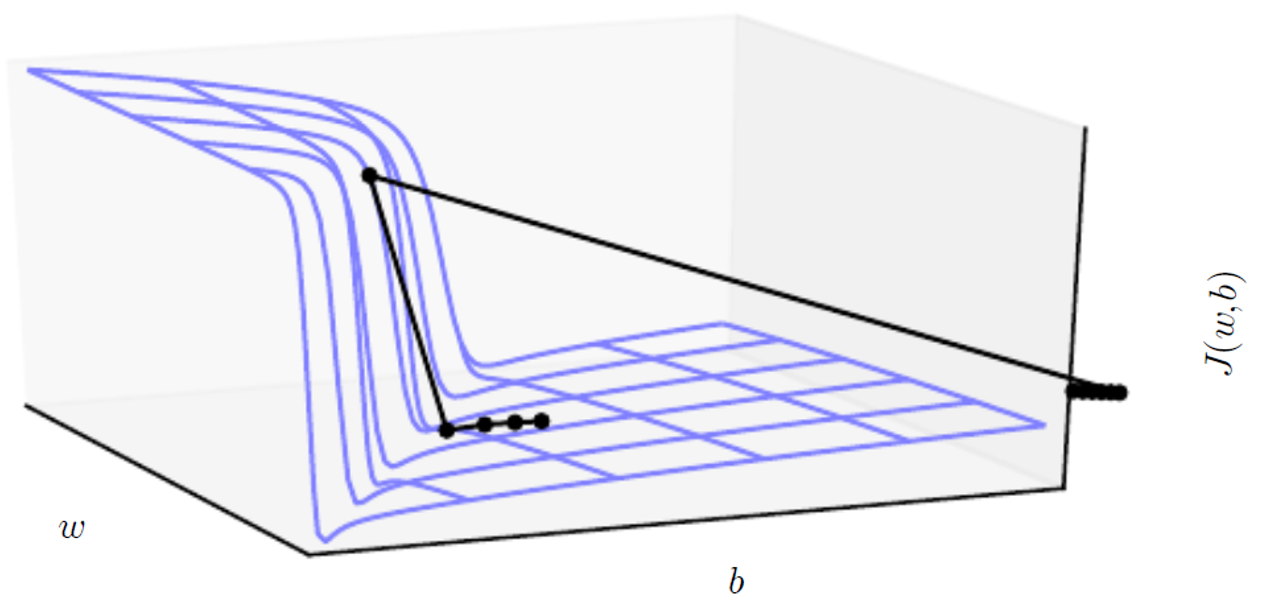
\includegraphics[width=0.9\linewidth]{images/cliff.png}
	\end{figure}


	\subsection{Long-Term Dependencies}
	Another difficulty that neural network optimization algorithms must overcome arises when the computational graph becomes extremely deep.
	Repeated application of the same parameters gives rise to especially pronounced diffculties.
	For example, suppose that a computational graph contains a path that consists of repeatedly multiplying by a matrix $\mW$.
	After $t$ steps, this is equivalent to multiplying by $\mW^t$.
	Suppose that $\mW$ has the following eigendecomposition:
	\begin{align*}
	\mW &= \mV \diag(\bol{\lambda})\mV^{-1}\\
	\mW^t &= \left(\mV \diag(\bol{\lambda})\mV^{-1}\right)^t = \mV \diag(\bol{\lambda})^t\mV^{-1}
 	\end{align*}


	In this simple case, it is straightforward to see that any eigenvalues $\lambda_i$ that are not near an absolute value of 1 will either explode if they are greater than 1 in magnitude or vanish if they are less than 1 in magnitude.\\

	The vanishing and exploding gradient problem refers to the fact that gradients through such a graph are also scaled according to $\diag(\bol{\lambda})^t$.
	\textbf{Vanishing gradients }make it difficult to know which direction the parameters should move to improve the cost function.
	\textbf{Exploding gradients} make learning unstable.

	\subsection{Algorithms with Adaptive Learning Rates \buch{Chapter 8.5}\buchSeite{298}}
		\subsubsection{Momentum}
		In all algorithms, we first calculate the gradient $g_t$ at time $t$ on a mini-batch of size $m$ with

		\[ g_{t} = \frac{1}{m} \nabla_{\Theta} \sum L(f(x^{(i)};\Theta),y^{(i)})    \]

		The final weight update is always given by

		\[ \Theta_{t} = \Theta_{t-1} + \Delta\Theta_{t} \]

		% The learning rate, if applicable, is denoted by $\theta$, and $\delta$ denotes a small constant (e.g. $ 10^{-6} $ or $ 10^{-8} $), which is required for numerical stability.

		\subsubsection{AdaGrad}
		The AdaGrad algorithm scales the learning rate of all model parameters by dividing them by the square root of the sum of all historical values of the gradient.

		\[ r_{t} = r_{t-1} + g_{t}\odot g_{t} \]
		\[ \Delta\Theta_{t} = - \frac{\eps}{\delta + \sqrt{r_{t}}} \odot g_{t} \]

		\subsubsection{RMSProp}
		The RMSProp algorithm is basically the same as AdaGrad, but the gradient is accumulated with an exponentially weighted moving average.

		\[ r_{t} = \rho r_{t-1} + (1- \rho) g_{t}\odot g_{t}\]
		\[ \Delta\Theta_{t} = - \frac{\eps}{\sqrt{\delta + r_{t}}} \odot g_{t} \]

		RMSProp combined with Nesterov momentum:

		\[ \tilde{\Theta_{t}} = \Theta_{t-1} + \alpha \Delta\Theta_{t-1} \]
		\[ g_{t} = \frac{1}{m} \nabla_{\tilde{\Theta_{t}}} \sum L(f(x^{(i)};\tilde{\Theta}),y^{(i)})    \]
		\[ r_{t} = \rho r_{t-1} + (1- \rho) g_{t}\odot g_{t}\]
		\[ \Delta\Theta_{t} = \alpha\Delta\Theta_{t-1} - \frac{\eps}{\sqrt{\delta + r_{t}}} \odot g_{t} \]

		\subsubsection{AdaDelta}
		AdaDelta is mentioned in the book, but not described. The idea is similar to RMSProp: the gradient is accumulated with an exponentially weighted moving average

		\[ r_{t} = \rho r_{t-1} + (1- \rho) g_{t}\odot g_{t}\]

		But now, we also accumulate the squared gradients using an exponentially weighted moving average

		\[ s_{t} = \rho s_{t-1} + (1 - \rho)\Delta\Theta_{t} \odot \Delta\Theta_{t} \]

		and use the accumulated squared gradient as the numerator in the gradient update

		\[ \Delta\Theta_{t} = - \frac{\sqrt{\delta + s_{t-1}}}{\sqrt{\delta + r_{t}}} \odot g_{t}\]

		Note that we first calculate the parameter update $ \Delta\Theta_{t} $ using the accumulated squared gradient of the last step $ s_{t-1} $, and then afterwards update the squared gradient $ s_{t} $. Thus, the accumulated squared gradient lags behind by one time step.\\
		AdaDelta has the advantage, that no learning rate $ \eps $ is required at all.

		\subsubsection{Adam}
		Adam (Adaptive Moments) goes one step further and accumulates the first- and second-order moments of the gradient to adapt the learning rate.

		\[ s_{t} = \rho_{1} s_{t-1} + (1 - \rho_{1})g_{t} \]
		\[ r_{t} = \rho_{2} r_{t-1} + (1 - \rho_{2})g_{t} \odot g_{t} \]

		The parameter update then uses the first-order moment of the gradient $ s_{t} $ instead of the gradient $ g_{t} $.

		\[ \Delta\Theta_{t} = -\eps\frac{\hat{s_{t}}}{\delta + \sqrt{\hat{r_{t}}}} \]

		Note that we use the bias-corrected versions $ \hat{s_{t}} = s_{t} / (1 - \rho_{1}^{t}) $ and $ \hat{r_{t}} = r_{t} / (1 - \rho_{2}^{t}) $, which are required due
		to the initialization at $ t = 0 $.

	\subsection{Batch Normalization}
	This is a method of adaptive re-parametrization, motivated by the difficulty of training very deep models.
	The gradient tells how to update each parameter, under the assumption that the other layers do not change.
	In practice, we update all of the layers simultaneously.
	When we make the update, unexpected results can happen because many functions composed together are changed simultaneously, using updates that were computed under the assumption that the other functions remain constant.\\

	Batch normalization provides a way of reparametrizing almost any deep network.
	The reparametrization significantly reduces the problem of coordinating updates across many layers.
	Batch normalization can be applied \textbf{to any input or hidden layer} in a network.\\

	Let $\mH$ be a minibatch of pre-activations of the layer to normalize arranged as a design matrix, with the pre-activations for each example appearing in a \textbf{row} of the matrix.
	To normalize $\mH$, we replace it with the expression
	\[ \mH'=\frac{\mH - \vmu}{\bol{\sigma}} \]

	The mean and the standard deviation per minibatch can be calculated during training:
	\begin{align*}
	\vmu &= \frac{1}{m}\sum_i\mH_{i,:}\\
	\bol{\sigma} &= \sqrt{\delta+\frac{1}{m}\sum_i (\mH-\vmu)_{i,:}^2}
	\end{align*}
	\textbf{Important:}
	We back-propagate through these operations for computing the mean and the standard deviation, and for applying them to normalize $\mH$. This means that the gradient will never propose an operation that acts simply to increase the standard deviation or mean of any pre-activation. The normalization operations remove the effect of such an action and zero out its component in the gradient. Hence the mean of the pre-activation stays at zero and the standard deviation at one over a minibatch, which solves many problems related to exploding and vanishing gradients.


	\subsection{Parameter Initialization Strategies \buch{Chapter 8.4}\buchSeite{292}}
	A few things to know about what the initialization does affect:
	\begin{itemize}
		\item Most algorithms are strongly affected by the choice of initialization
		\item The initial point can determine whether the algorithm converges at all
		\item When learning does converge, the initial point can determine how quickly learning converges and whether it converges to a point with high or low cost
		\item Also, points of comparable cost can have wildly varying generalization error, and the initial point can affect the generalization as well
	\end{itemize}

	The initialization strategies used today are simple and heuristic. Hence we don't know much about
	how the initial point affects generalization. So there's little to no guidance how to select the initial point of the parameters.\\
	The only property known with complete certainty is that the initial parameters need to “break symmetry” between different units. If two hidden units with the same activation function are connected to the same inputs leads during training to constantly update both of these units in the same way.\\
	The goal of having each unit compute a different function motivates	random initialization of the parameters. Typically we set the biases for each unit to a heuristically chosen constant (0 is popular (0.1 for ReLu)).We almost always initialize all the weights in the model to values drawn randomly from a Gaussian or uniform distribution.\\
	\textbf{Larger initial }weights will yield a stronger symmetry breaking effect, helping to avoid redundant units. They also help to avoid losing signal during forward- or back-propagation through the linear component of each layer. If the initial weights get \textbf{too large} it can result in exploding values during forward- or back-propagation (Maybe clipping gradient can be used to avoid those effects).\\

	A heuristic is to initialize the weights of a fully connected layer with m inputs and n outputs by sampling each weight from the uniform distribution shown below. Which leads to:
	\[  U(-\frac{\sqrt{3}}{\sqrt{m}}, \frac{\sqrt{3}}{\sqrt{m}}) \]

	\begin{figure}[H]
		\centering
		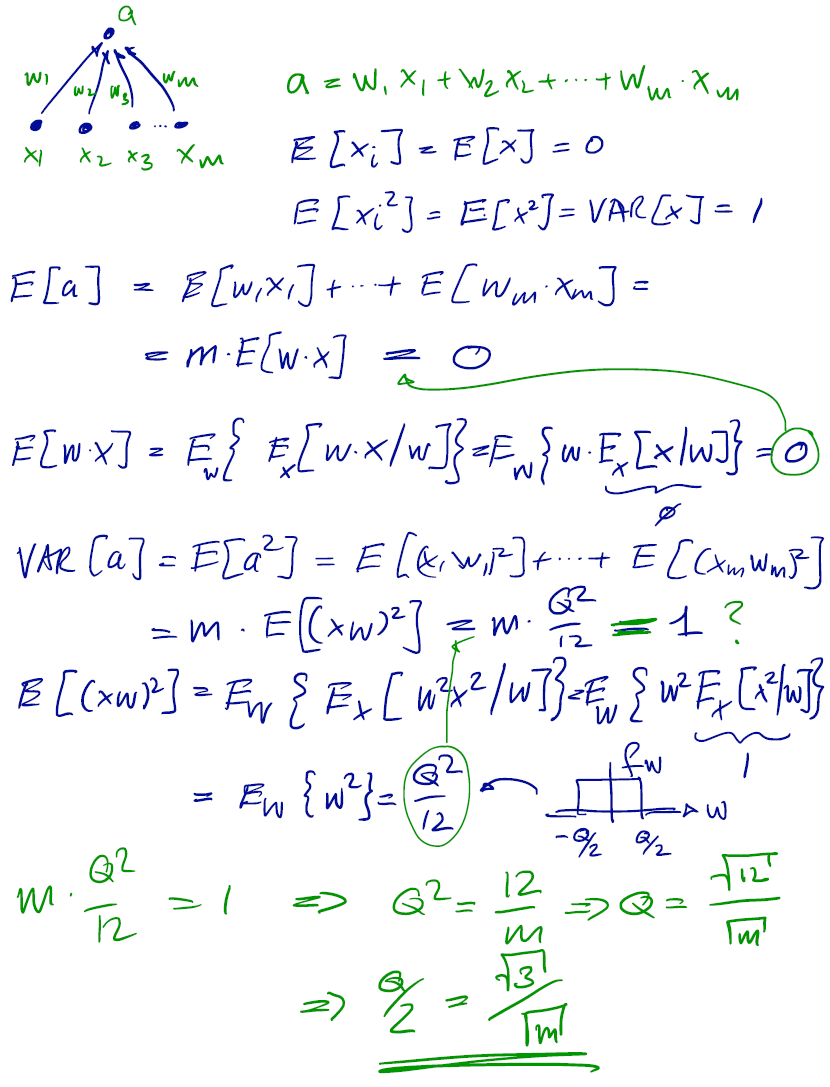
\includegraphics[width=0.9\linewidth]{images/InitStrat.png}
	\end{figure}

	Normalized initialization: This heuristic is designed to compromise between the goal of initializing all layers to have the same pre-activation variance and the goal of initializing all layers to have the same gradient variance. The formula is derived using the assumption that the network consists only of a chain of matrix multiplications, with no nonlinearities.

	\[ W_{i,j} \sim\ U ( -\frac{\sqrt{6}}{\sqrt{m + n}}, \frac{\sqrt{6}}{\sqrt{m + n}} )  \]

	This strategy is often called the \textbf{Xavier Initialization}.\\
	There are some more strategies which are often applied in neural networks which we will not go into further details.



	\newpage
\end{multicols}

\section{Convolutional Networks}
\begin{multicols}{2}
	\subsection{The convolutional Operation}
	Convolutional Neural Networks (CNNs) are a kind of neural networks for processing data that has a known, grid-like topology.
	Examples include time-series data, which can be thought of as a 1D grid taking samples at regular time intervals, and image data, which can be thought of as a 2D grid of pixels.
	They are very popular for image processing and hence the both often refers to images and pixels, but they can be used for any dimensional input.\\
	
	The name CNN indicates that the network employs a mathematical operation called \textbf{convolution}.
	Convolutional networks are neural networks that use convolution in place of general matrix multiplication in at least one of their layers.\\
	
	If we have a 1D measurement over time and we want to reduce the noise, we can average the sampled data.
	More recent measurements are more relevant, so we will want this to be a weighted average that gives more weight to recent measurements.
	We can do this with a weighting function $w(a)$, where $a$ is the age of a measurement point:
	\[ s(t) = \int x(a)w(t-a)da \]
	If we apply such a weighted average operation at every moment, we obtain a new function $s$ providing a smoothed estimate of the position:
	\[ s(t) = (x\ast w)(t) \]
	
	$w()$ needs to be a valid probability density function, otherwise the output is not a weighted average.
	$w()$ also needs to be zero for all negative arguments, otherwise it will look into the future (acausal).\\
	If we work with sampled data, we need to work with discrete convolution, hence $t$ and $a$ are now integers and the integral becomes a summation
	\[ s(t) = (x\ast w)(t) = \sum_{a=-\infty}^{\infty} x(a)w(t-a) \]
	
	We often use convolutions over more than one axis at a time.
	For example, if we use a two-dimensional image $\mI$ as our input, we probably also want to use a two-dimensional kernel $\mK$.
	\begin{align*}
		S(i,j)
		&= (I\ast K)(i,j) &= \sum_m\sum_n I(m,n) K(i-m,j-n)\\
		&= (K\ast I)(i,j) &= \sum_m\sum_n I(i-m,j-n) K(m,n)
	\end{align*}
	
	Usually the formula in the last line is more straightforward to implement, because there is less variation in range of valid values of $m$ and $n$.
	\begin{figure}[H]
		\centering
		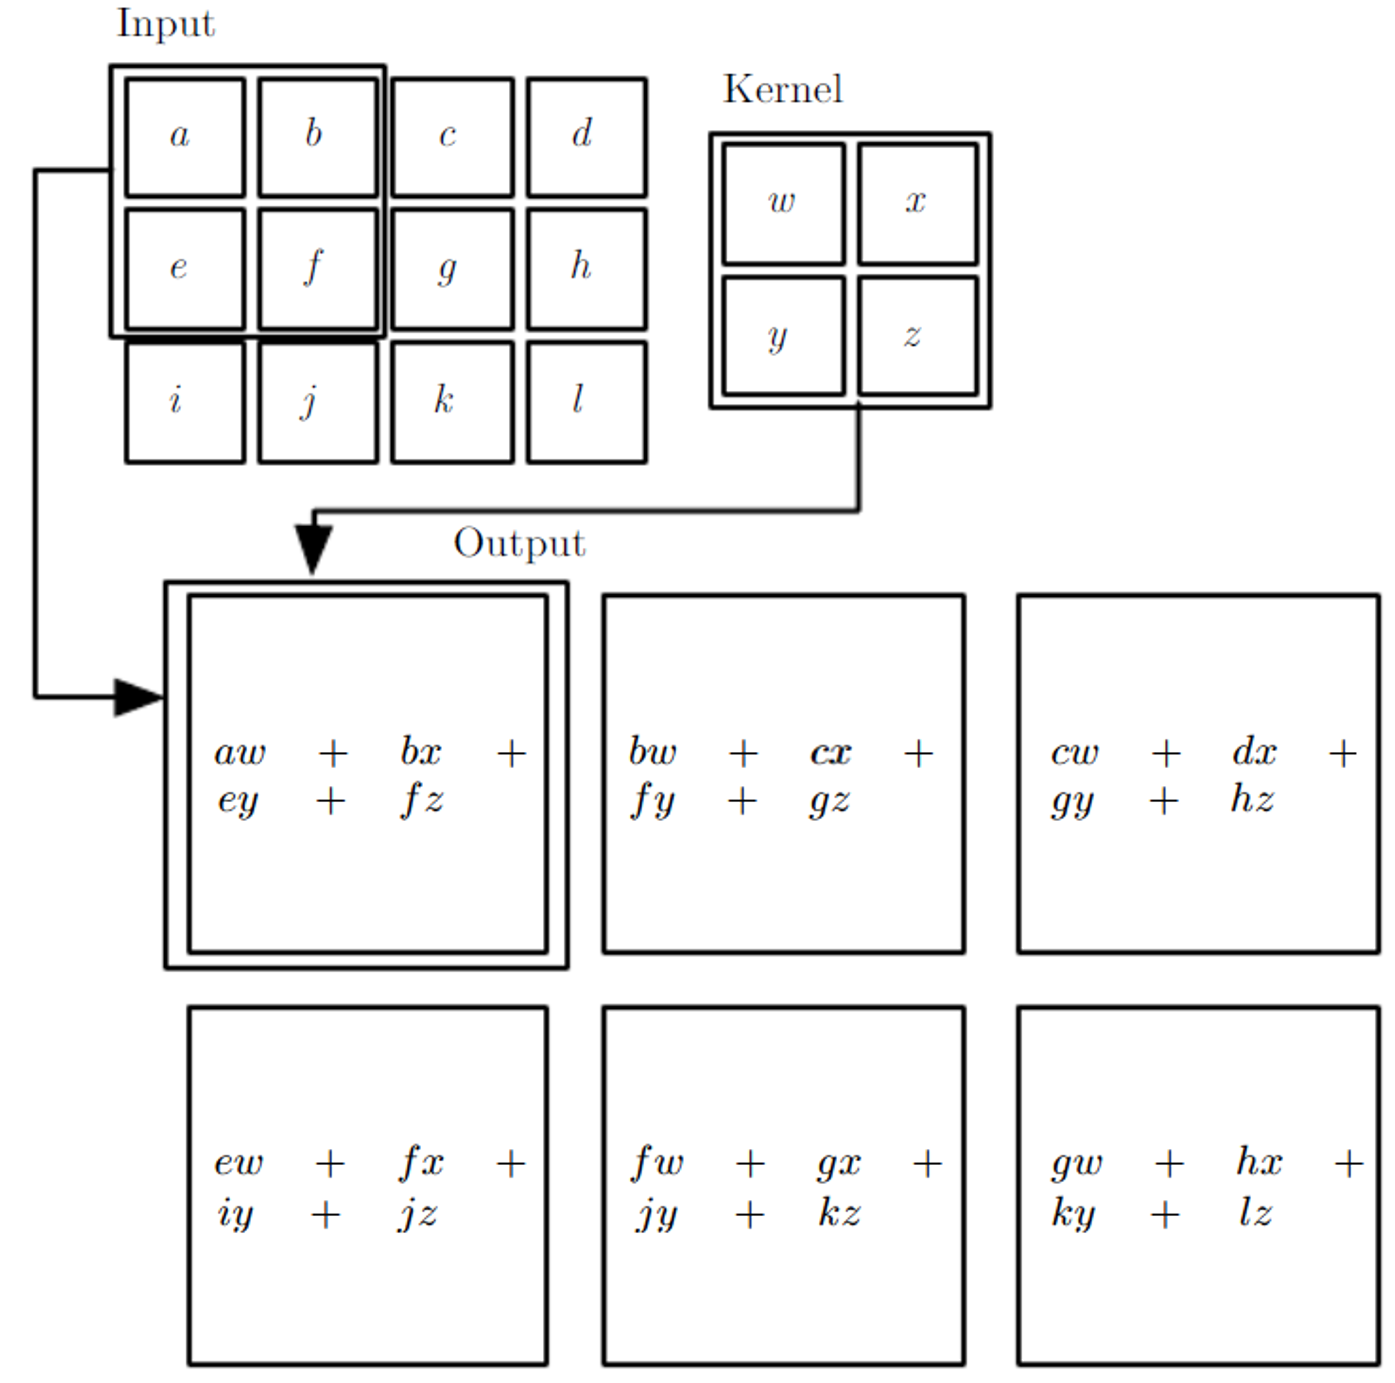
\includegraphics[width=0.65\linewidth]{images/2dconv.PNG}
	\end{figure}
	\subsection{Motivation}
	CNNs typically have \textbf{sparse interactions} (also referred to as sparse connectivity or sparse weights).
	This is accomplished by making the kernel smaller than the input.
	\begin{figure}[H]
		\centering
		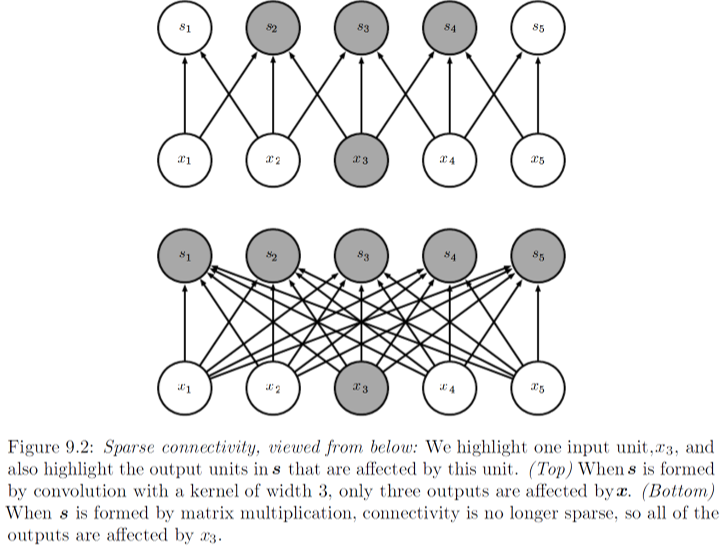
\includegraphics[width=0.85\linewidth]{images/sparse1.png}
	\end{figure}
	\begin{figure}[H]
		\centering
		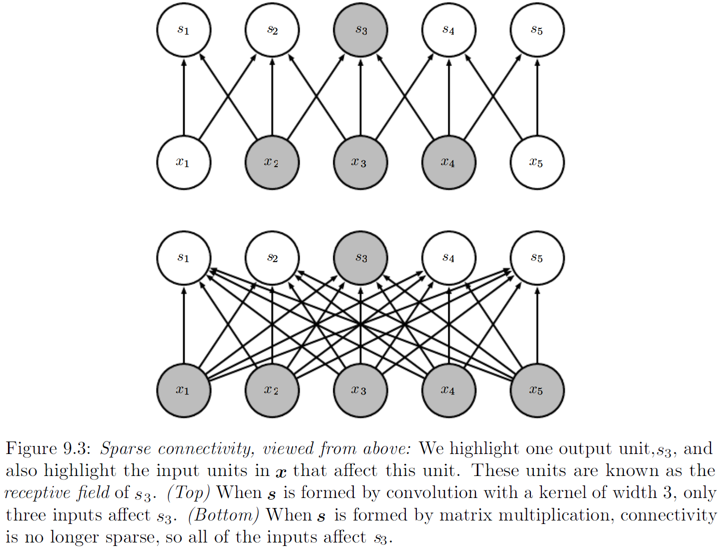
\includegraphics[width=0.85\linewidth]{images/sparse2.png}
	\end{figure}
	
	\textbf{Parameter Sharing} refers to using the same parameter for more than one function in a model.
	In a traditional neural net, each element of the weight matrix is used exactly once when computing the output of a layer.
	In a CNN, each member of the kernel is used at every position of the input.
	The parameter sharing used by the convolution operation means that rather than learning a separate set of parameters for every location we learn only one set.\\
	
	This does not affect the runtime of forward propagation but it does further reduce the storage requirements of the model to $k$ parameters.
	Convolution is thus dramatically more efficient than dense matrix multiplication in terms of the memory requirements and statistical efficiency.\\
	
	Convolution is \textbf{equivariant to translation}.
	This implies that when the input is moved by a certain amount, the output of the convolution is also moved by the same amount in the same direction.
	When processing time series data, this means that convolution produces a sort of timeline that shows when different features appear in the input.
	If we move an event later in time in the input, the exact same representation of it will appear in the input, just later in time.\\
	Similarly with images, convolution creates a 2D map of where certain features appear in the input. If we move the object in the input, its representation will move the same amount in the output.\\
	
	\subsection{Pooling}
	A typical layer of a CNN consists of three stages:
	\begin{itemize}
		\item In the first stage, the layer performs several convolutions in parallel to produce a set of linear activations
		\item In the second stage, each linear activation is run through a nonlinear activation function, such as the rectified linear activation function (detector stage)
		\item In the third stage, we use a pooling function to modify the output of the layer further. A pooling function replaces the output of the net at a certain location with a \textbf{summary statistic} of the nearby outputs
	\end{itemize}
	Typical pooling function over (mostly rectangular) neighborhoods:
	\begin{itemize}
		\item \textbf{Max pooling} Reports the maximum output
		\item\textbf{Average pooling} Reports the average output	
		\item\textbf{Weighted average pooling} Reports a weighted average based on the distance from the central point
		\item\textbf{$L^2$ norm pooling} Reports the $L^2$ norm of a neighborhood
	\end{itemize}
	Pooling helps to make the representation become approximately invariant to small translations of the input.
	If we pool over the outputs of separately parametrized convolutions, the features can learn which transformations to become invariant to.
	\begin{figure}[H]
		\centering
		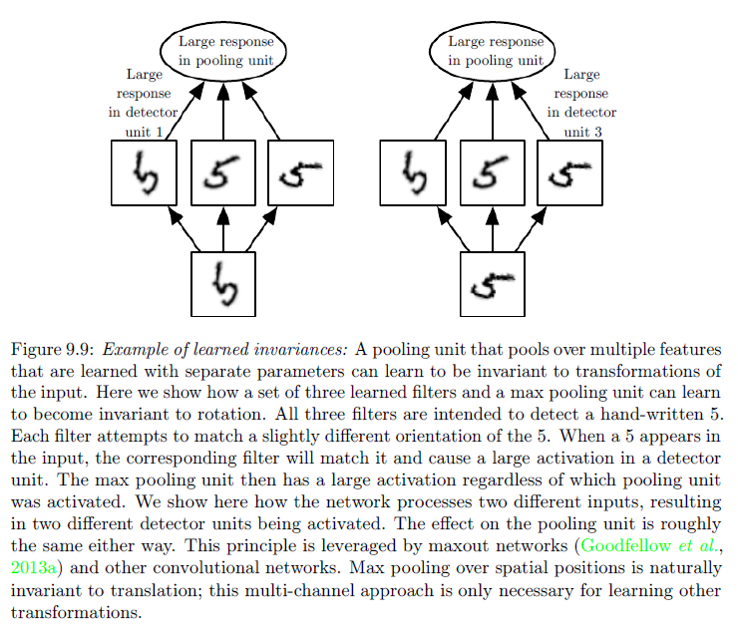
\includegraphics[width=0.8\linewidth]{images/pooling.png}
	\end{figure}
	Pooling and downsampling are essential for handling inputs of varying size.
	For example, if we want to classify images of variable size, the input to the classification layer must have a fixed size.
	This is usually accomplished by varying the size of an offset between pooling regions (called \textbf{stride}) so that the classification layer always receives the same number of summary statistics, regardless of the input size.
	\begin{figure}[H]
		\centering
		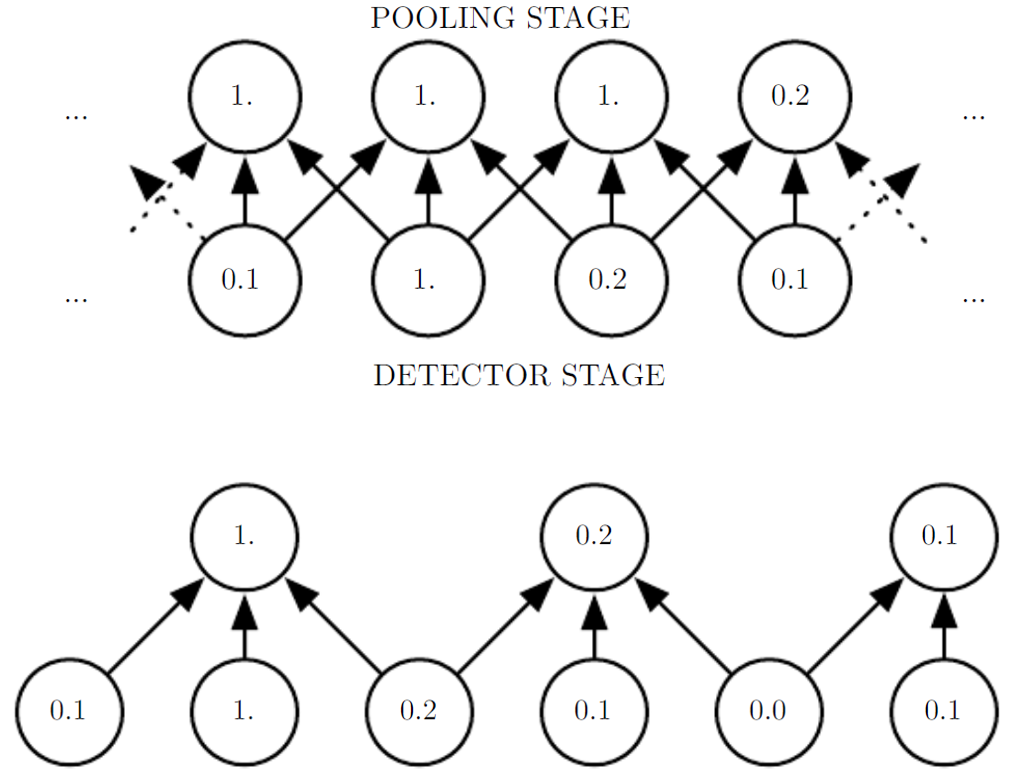
\includegraphics[width=0.8\linewidth]{images/stride.PNG}
	\end{figure}
	\begin{figure}[H]
		\centering
		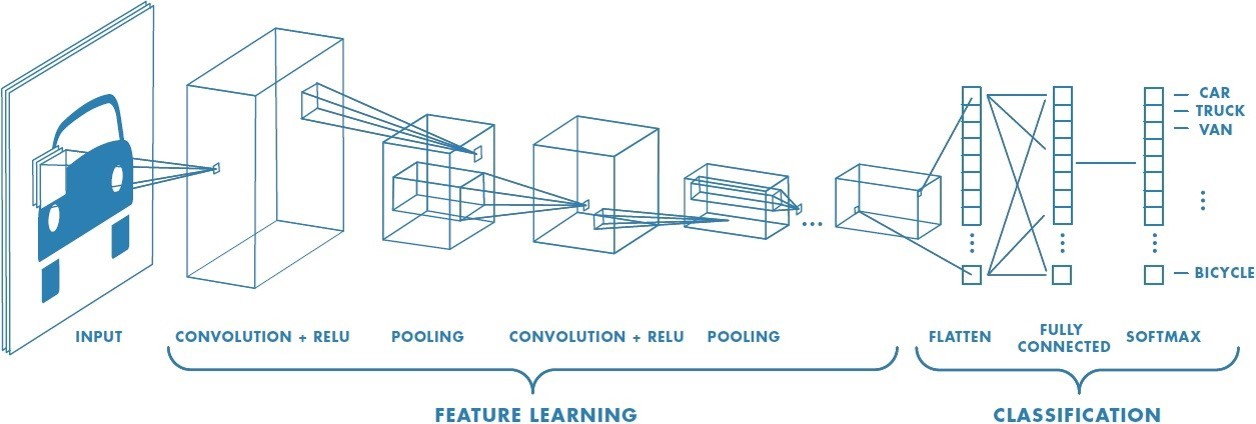
\includegraphics[width=0.9\linewidth]{images/cnn_arch.jpg}
	\end{figure}
	\newpage
	\subsection{Variants of the Basic Convolution Function}
	Assume we have a 4D kernel tensor $\tK$ with element $\etK_{i,j,k,l}$ giving the connection strength between a unit in channel $i$ of the output and a unit in channel $j$ of the input, with an offset of $k$ rows und $l$ columns between the output and input unit.\\
	Assume our input consists of observed data $\tV$ with element $\etV_{i,j,k}$ giving the value of the input unit within channel $i$ at row $j$ and column $k$.
	\[ \tZ_{i,j,k} = \sum_{l,m,n} \etV_{l,j+m-1,k+n-1} \etK_{i,l,m,n} \]
	
	Choosing a stride bigger than one results in reduction of computational cost.
	We can think of this as \textbf{downsampling} the output of the full convolution function.\\
	If we want to sample only every $s$ (stride) pixels in each direction in the output, then we can define a downsampled convolution function $c$ as 
	\[ \etZ_{i,j,k} = c(\tK,\tV,s)_{i,j,k} = \sum_{l,m,n}\left[ \etV_{l,(j-1)\times s+m,(k-1)\times s+n} \etK_{i,l,m,n} \right] \]
	\begin{figure}[H]
		\centering
		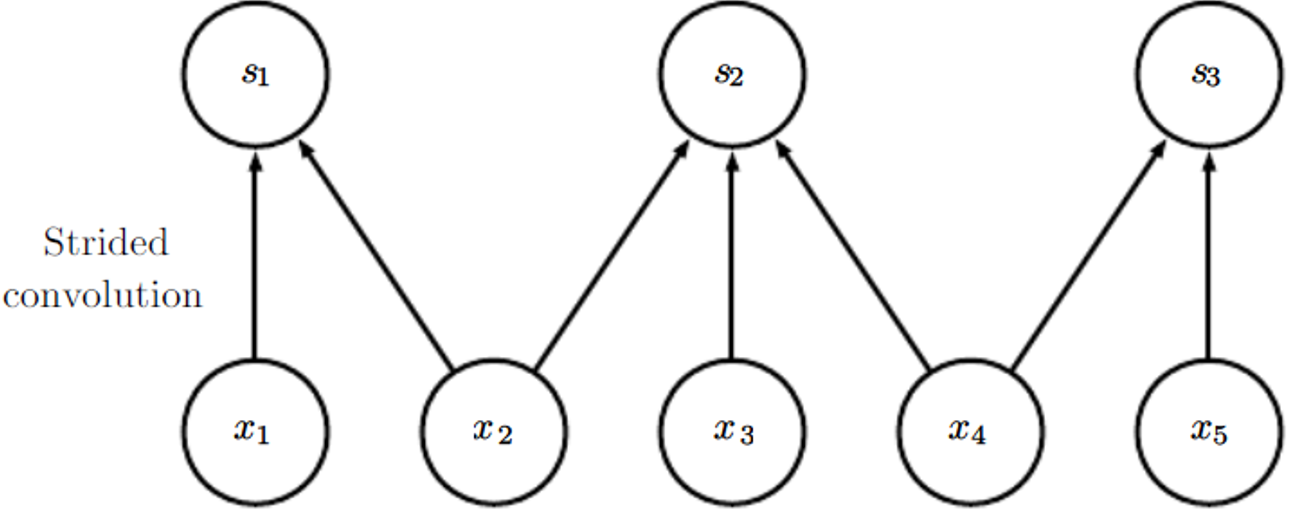
\includegraphics[width=0.5\linewidth]{images/strided_conv.PNG}
	\end{figure}
	
	One essential feature of any CNN implementation is the ability to\textbf{ implicitly zero-pad} the input $\tV$ in order to make it wider.
	Without this feature, the width of the representation shrinks by one pixel less than the kernel width at each layer:
	\[ \underbrace{(m\times n)}_{\text{Input}} \ast \underbrace{(k\times k)}_{\text{Kernel}} = 
	\underbrace{\left( (m-k+1)\times (n-k+1) \right)}_{\text{Output}} \]
	Three special cases of zero-padding:
	\begin{enumerate}
		\item No zero-padding, therefore the convolution kernel is only allowed to visit position where the entire kernel is contained \textbf{entirely} within the image. In MATLAB terminology, this is called \textbf{valid} convolution. In this case, all pixels in the output are a function of the same number of pixels in the input.
		\item Just enough zero-padding is added to keep the size of the output equal to the size of the input. MATLAB calls this \textbf{same} convolution. In this case, the network can contain as many convolutional layers as the available hardware can support. However, the input pixels near the border influence fewer output pixels than the input pixels further to the center. This can make the border pixels somewhat underrepresented in the model.
		\item The last one is called \textbf{full} convolution (in MATLAB), where enough zeroes are added for every pixel to be visited $k$ times in each direction, resulting in an output image of width $m+k-1$. In this case, the output pixels near the border are a function of fewer pixels than the output pixels near the center. This can make it difficult to learn a single kernel that performs well at all positions in the convolutional feature map.
		\item[$\rightarrow$] Usually, the optimal amount of zero padding (in terms of test set classification accuracy) lies somewhere \textbf{between valid and same} convolution.
	\end{enumerate}

	\textbf{Locally connected layers}  are not convolutional layers, even though they are locally connected but not with shared weights.
	In this case, the adjacency matrix in the MLP graph is the same, but every connection has its own weight, specified by a 6D tensor $\tW$.
	The indices into $\tW$ are respectively:
	$i$ the output channel, $j$ the output row, $k$ the output column, $l$ the input channel, $m$ the row offset within the input, $n$ the column offset within the input.
	The linear part of a locally connected layer is given by
	\[ \etZ_{i,j,k} = \sum_{l,m,n} \left[ \etV_{l,j+m-1,k+n-1} \etW_{i,j,k,l,m,n} \right] \]
	This is sometimes also called \textbf{unshared convolution}, because it is a similar operation to discrete convolution with a small kernel, but without sharing parameters across locations.
	Locally connected layers are useful when we know that each feature should be a function of a small part of space, but there is no reason to think that the same feature should occur across all of space.
	For example, if we want to tell if an image is a picture of a face, we only need to look for the mouth in the bottom half of the image.
	\begin{figure}[H]
		\centering
		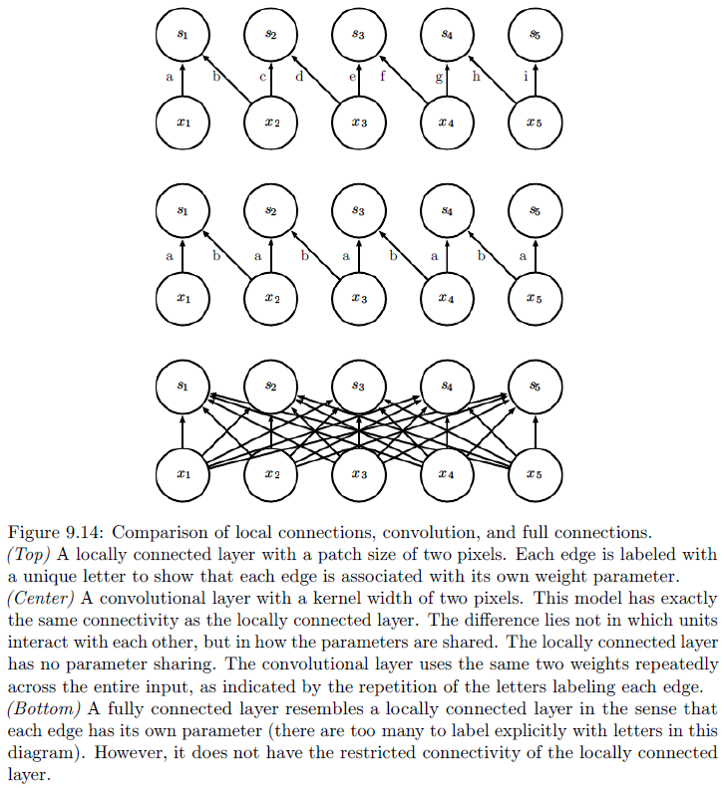
\includegraphics[width=0.8\linewidth]{images/locallyConn.png}
	\end{figure}
	\newpage
	\subsection{Data Types}
	The data used with a CNN usually consists of several channels, each channel being the observation of a different quantity at some point in space or time.
	\begin{figure}[H]
		\centering
		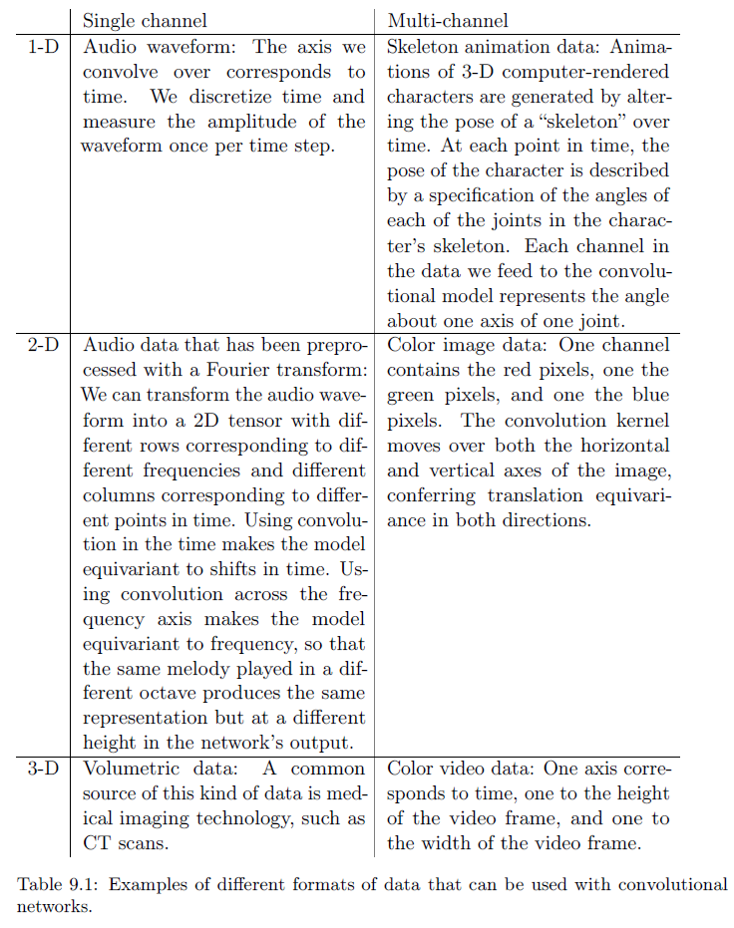
\includegraphics[width=\linewidth]{images/datatypes.png}
	\end{figure}
	
	One advantage to CNNs is that they can also process inputs with \textbf{varying spatial extents}.
	These kinds of input simply cannot be represented by traditional, matrix multiplication-based neural networks.
	Sometimes the output of the network is allowed to have variable size as well as the input, for example if we want to assign a class label to each pixel of the input.
	In other cases, the network must produce some fixed-size output, for example if we want to assign a single class label to the entire image. In this case, we must make some additional design steps, like inserting a pooling layer whose \textbf{pooling regions scale in size proportional to the size of the input}, in order to maintain a fixed number of pooled outputs.
	\columnbreak
	\subsection{Efficient Convolution Algorithms}
	Convolution is equivalent to converting both the input and the kernel to the frequency domain using a \textbf{Fourier transform (FFT)}, performing point-wise multiplication of the two signals, and converting back to the time domain using an inverse Fourier transform. For some problem sizes, this can be faster than the naive implementation of discrete convolution.\\
	
	When a d-dimensional kernel can be expressed as the outer product of d vectors, one vector per dimension, the kernel is called \textbf{separable}.
	Not only are two 1D convolutions much faster than one 2D convolution, the kernel also takes fewer parameters to represent as vectors.
	If the kernel is $w$ elements wide in each dimension, then naive multidimensional convolution requires $O(w^d)$ runtime and parameter storage space, while separable convolution requires $O(w\cdot d)$ runtime and parameter storage space.
	
	\begin{figure}[H]
		\centering
		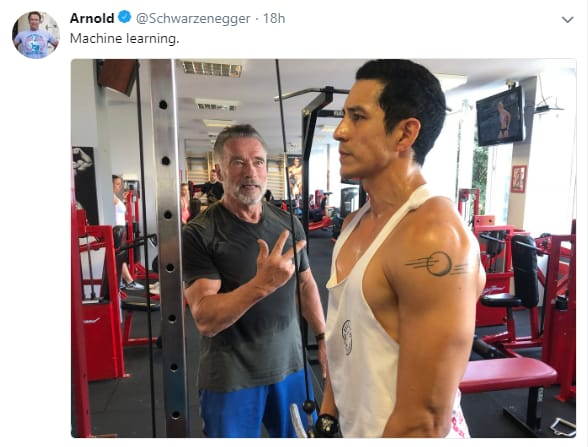
\includegraphics[width=0.9\linewidth]{images/arni.jpeg}
	\end{figure}
	
\end{multicols}

\newpage




































\section{Sequence Modeling: Recurrent and Recursive Nets}
\begin{multicols}{2}
	\subsection{Recurrent Nets}
	A recurrent neural network (\textbf{RNN}) is a neural network that is specialized for processing a sequence of values $\vx^{(1)},\dots,\vx^{(\tau)}$.
	They can scale to much longer sequences than would be practical for networks without sequence-based specialization.
	Most RNNs can also process sequences of variable length.
	Just as for CNNs, a large part of the power comes from \textbf{parameter sharing}.
	If we had separate parameters for each value of the time index, we could not generalize to sequence lengths not seen during training.
	\begin{figure}[H]
		\centering
		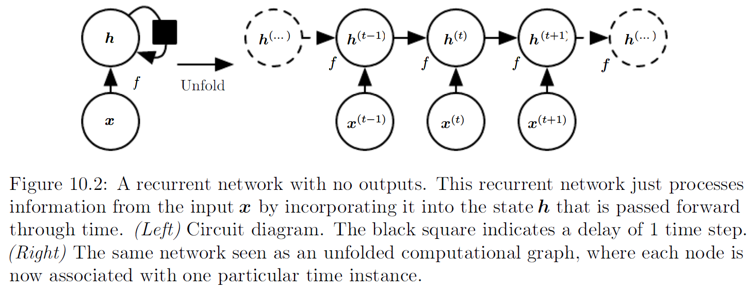
\includegraphics[width=\linewidth]{images/recurr1.png}
	\end{figure}

	RNNs share parameters in a different way than CNNs.
	Each member of the output is a function of the previous members of the output.
	Each member of the output is produced using the same update rule applied to the previous outputs.
	This recurrent formulation results in the sharing of parameters through a very deep computational graph.\\

	We refer to RNNs as operating on a sequence that contains vectors $\vx(t)$ with time step index $t$ ranging from 1 to $\tau$.
	In practice, RNNs usually operate on minibatches of such sequences, with a different sequence length $\tau$ for each member of the minibatch.
	RNNs may also be applied in two dimensions across spatial data such as images, and even when applied to data involving time, the network may have connections that go backwards in time, provided that the entire sequence is observed before it is provided to the network.

	\subsection{Unfolding Computational Graphs}
	A computational graph is a way to formalize the structure of a set of computations, such as those involved in mapping inputs and parameters to outputs and loss.
	The idea of unfolding a recurrent computation into a computational graph that has a repetitive structure, typically corresponding to a chain of events.
	Unfolding this graph results in the sharing of parameters across a deep network structure.
	\begin{align*}
	\vs^{(t)} &= f\left(\vs^{(t-1)};\bolt\right)\\
	\vs^{(3)} &= f\left(\vs^{(2)};\bolt\right)\\
	&= f\left(f\left(\vs^{(1)};\bolt\right);\bolt\right)
	\end{align*}
	As another example, let us consider a dynamical system driven by an external signal $\vx^{(t)}$ with state $\vs^{(t)}$
	\[ \vs^{(t)} = f\left(\vs^{(t-1)},\vx^{(t)};\bolt\right) \]
	where we see that the state now contains information about the whole past sequence.\\

	To indicate that the state is the hidden units in the network, we now rewrite the equation using the variable $\vh$ to represent the (hidden) state:
	\[ \vh^{(t)} = f\left(\vh^{(t-1)},\vx^{(t)};\bolt\right) \]
	When the recurrent network is trained to perform a task that requires predicting the future from the past, the network typically learns to use $\vh^{(t)}$ as a kind of lossy summary of the task-relevant aspects of the past sequence of inputs up to $t$.
	This summary is in general necessarily lossy, since it maps an arbitrary length sequence $\vx^{(t)},\vx^{(t-1)},\dots,\vx^{(1)}$ to a fixed length vector $\vh^{(t)}$.\\

	We can represent the unfolded recurrence after $t$ steps with a function $g^{(t)}$. This function takes the whole past sequence as input and produces the current state.
	The unfolded recurrent structure allows us to factorize $g^{(t)}$ into repeated applications of a function $f$.
	\begin{align*}
	\vh^{(t)} &= g^{(t)}\left( \vx^{(t)},\vx^{(t-1)},\vx^{(t-2)},\dots,\vx^{(2)},\vx^{(1)} \right)\\
	&= f\left(\vh^{(t-1)},\vx^{(t)};\bolt\right)
	\end{align*}
	One major advantage of RNNs is, that it's possible to use the \textbf{same} transition function $f$ with the same parameters at every time step.
	Another one is, that regardless of the sequence length, the learned model always has the same input size, because it is specified in terms of transition from one state to another state, rather than specified in terms of a variable-length history of states.

	\subsection{Recurrent Neural Networks}
	There is a wide array of RNNs possible.\\
	RNNs that produce an output at each time step and have recurrent connections between hidden units:
	\begin{figure}[H]
		\centering
		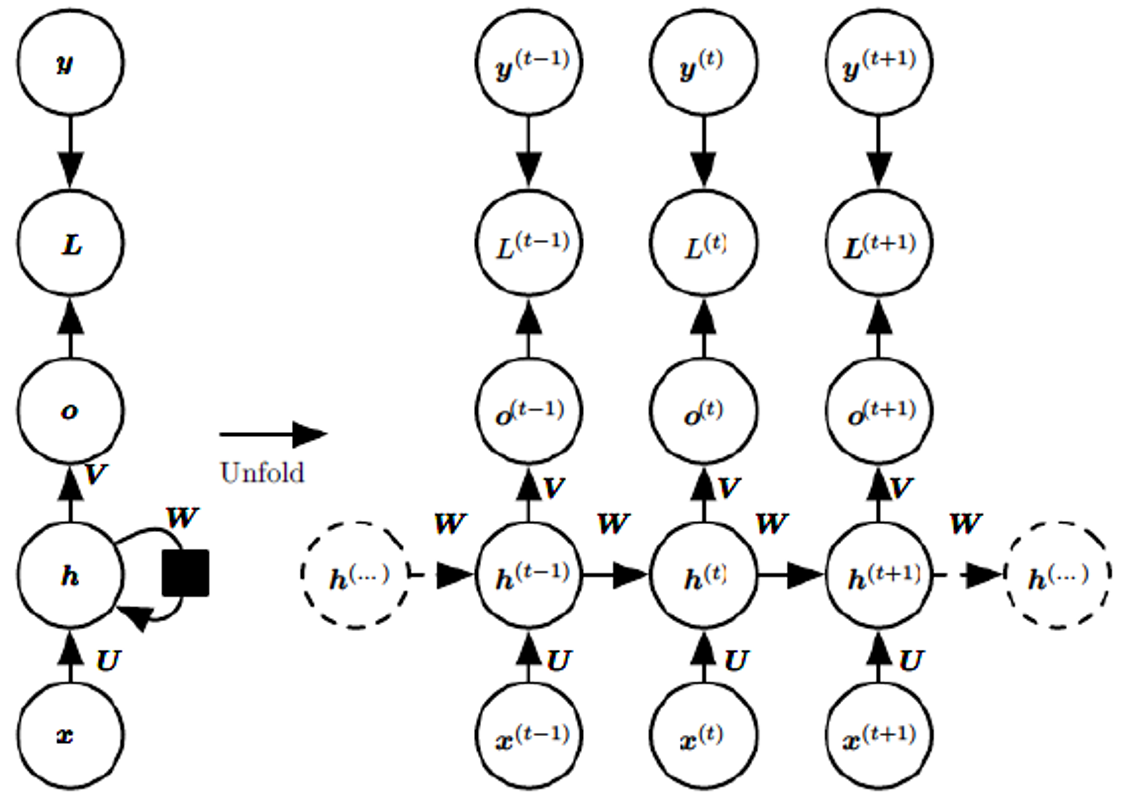
\includegraphics[width=0.8\linewidth]{images/rec1.PNG}
		\caption{This is the RNN we will refer to later}
	\end{figure}
	RNNs that produce an output at each time step and have recurrent connections only from the output at one time step to the hidden units at the next time step:
	\begin{figure}[H]
		\centering
		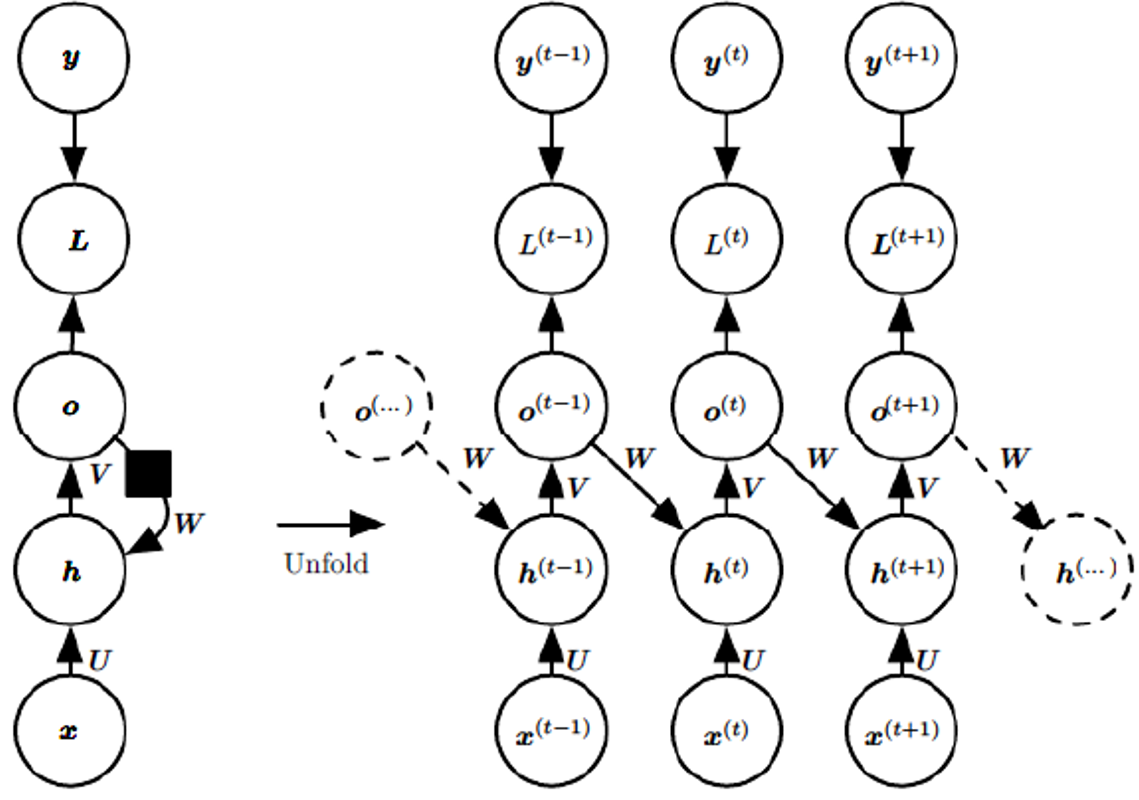
\includegraphics[width=0.8\linewidth]{images/rec2.PNG}
	\end{figure}
	RNNs with recurrent connections between hidden units, that read an entire sequence and then produce a single output:
	\begin{figure}[H]
		\centering
		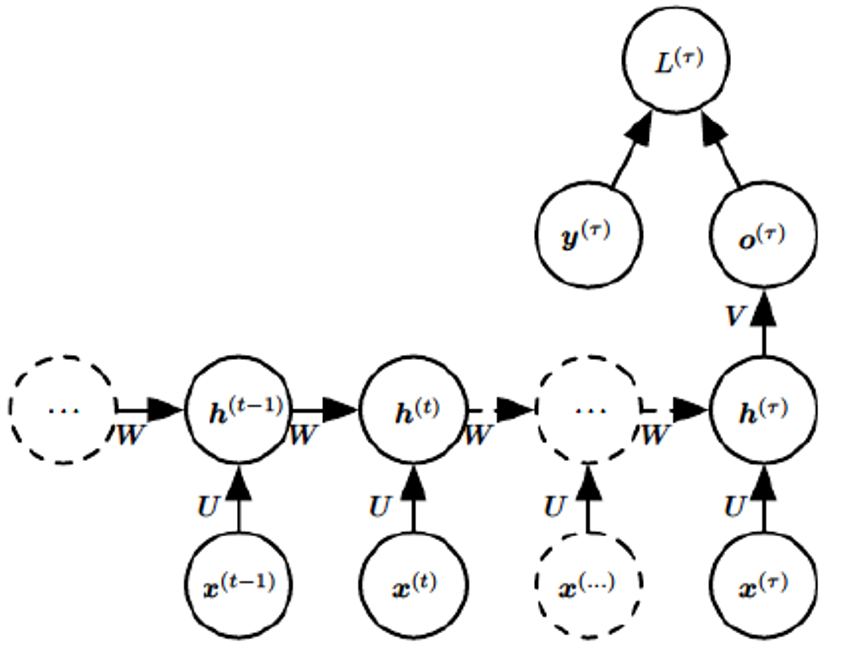
\includegraphics[width=0.7\linewidth]{images/rec3.PNG}
	\end{figure}

	\textbf{Forward propagation} begins with a specification of the initial state $\vh^{(0)}$.
	Then, for each time step from $t=1$ to $t=\tau$, we apply the update equations
	\begin{align*}
	\va^{(t)} &= \vb+\mW\vh^{(t-1)} +\mU\vx^{(t)}\\
	\vh^{(t)} &= \tanh(\va^{(t)})\\
	\vo^{(t)} &= \vc+\mV\vh^{(t)}\\
	\hat{\vy}^{(t)} &= \softmax(\vo^{(t)})
	\end{align*}
	where the parameters are the bias vectors $\vb$ and $\vc$, along with the weight matrices $\mU$, $\mV$ and $\mW$, respectively, for input-to-hidden, hidden-to-output and hidden-to-hidden connections.\\

	In figure 1 is an example of an RNN that maps an input sequence to an output sequence of the same length.
	The total loss for a given sequence of $\vx$ values paired with a sequence of $\vy$ values would then be just the sum of the losses over all the time steps.
	For example, if $L^{(t)}$ is the negative log-likelihood of $y^{(t)}$, given $\vx^{(1)},\dots,\vx^{(t)}$, then the loss function is calculated as
	\begin{align*}
	& L\left( \{ \vx^{(1)},\dots,\vx^{(\tau)} \}, \{ \vy^{(1)},\dots,\vy^{(\tau)} \} \right)\\
	&= \sum_t L^{(t)}\\
	&= -\sum_t \log p_{\text{model}}\left(y^{(t)}| \{ \vx^{(1)},\dots,\vx^{(t)} \} \right)
	\end{align*}
	$y^{(t)}$ is the current discrete desired output element (for example a word).
	The output of the softmax is a vector containing the estimated probabilities for each possible discrete output element (for example a word or a character).\\

	Computing the gradient for a typical RNN of this loss function with respect to the parameters is an expensive operation.
	The gradient computation involves performing a forward propagation pass moving left to right through the figure 1, followed by a backward propagation pass moving right to left through the graph.
	The runtime is $O(\tau)$ and cannot be reduced by parallelization because the forward propagation is inherently sequential; each time step may only be computed after the previous one.
	States computed in the forward pass must be stored until they are reused during the backward pass, so the memory cost is also $O(\tau)$.\\

	Gradients might explode, when the RNN is computed over many time steps.
	To avoid this, the update must be chosen to be small enough to avoid traversing too much upward curvature.
	We typically use learning rates that decay slowly enough that consecutive steps have approximately the same learning rate.
	A step size that is appropriate for a relatively linear part of the landscape is often inappropriate and causes uphill motion if we enter a more curved part of the landscape on the next step.
	\begin{figure}[H]
		\centering
		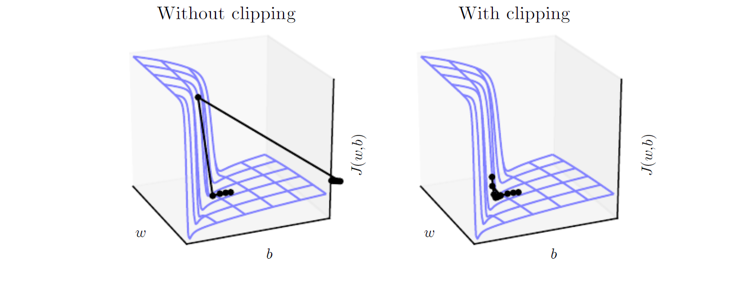
\includegraphics[width=0.9\linewidth]{images/clipping.png}
	\end{figure}
	One option is to \textbf{clip} the parameter gradient from a minibatch element-wise just before the parameter update.
	Another is to clip the norm of the gradient just before the parameter update:
	\[ \text{if } \lVert\vg\rVert > v \qquad\rightarrow\qquad \vg \leftarrow\frac{\vg v}{\lVert\vg\rVert} \]
	Although the parameter update has the same direction as the true gradient, with gradient norm clipping, the parameter update vector norm is now bounded.

	\subsection{Bidirectional RNNs}
	In many applications we want to output a prediction of $y^{(t)}$ which may depend on the \textbf{whole input sequence}.
	For example, in speech recognition, the correct interpretation of the current sound as a phoneme may depend on the next few phonemes because of co-articulation.
	Bidirectional RNNs combine an RNN that moves forward through time beginning from the start of the sequence with another RNN that moves backward through time beginning from the end of the sequence.
	\begin{figure}[H]
		\centering
		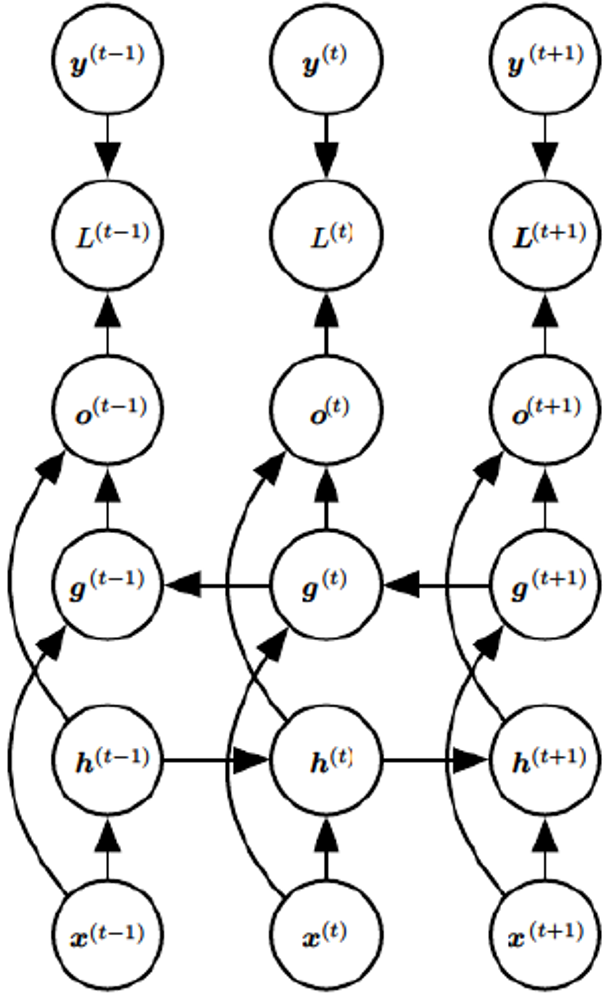
\includegraphics[width=0.4\linewidth]{images/bidir.PNG}
	\end{figure}
	The figure above illustrates the typical bidirectional RNN, with $\vh^{(t)}$ standing for the state of the sub-RNN that moves forward through time and $\vg^{(t)}$ standing for the state of the sub-RNN that moves backward through time.
	This allows the output units $\vo^{(t)}$ to compute a representation that depends on both the past and the future but is most sensitive to the input values around time $t$, without having to specify a fixed-size window around $t$.\\

	This idea can be naturally extended to a 2D input, such as images, by having four RNNs, each one going in one of the four directions.
	At each point $(i,j)$ of a 2D grid, an output could then compute a representation that would capture mostly local information but could also depend on long-range inputs.
	Compared to a CNN, RNNs applied to images are typically more expensive but allow for long-range lateral interactions between features in the same feature map.

	\subsection{Encoder-Decoder Sequence-to-Sequence Architectures}
	Mapping input sequences to output sequences of different lengths.
	We often call the input to the RNN the \textbf{context}. We want to produce a representation of this context, $\mC$. The context $\mC$ might be a vector or sequence of vectors that summarize the input sequence.\\
	In a sequence-to-sequence architecture, the two RNNs are trained jointly to maximize the average of the log conditional probability on the right over all the pairs of $\vx$ and $\vy$ sequences in the training set.
	\[ \log P(\vy^{(1)},\dots,\vy^{(n_y)}|\vx^{(1)},\dots,\vx^{(n_x)}) \]
	\begin{figure}[H]
		\centering
		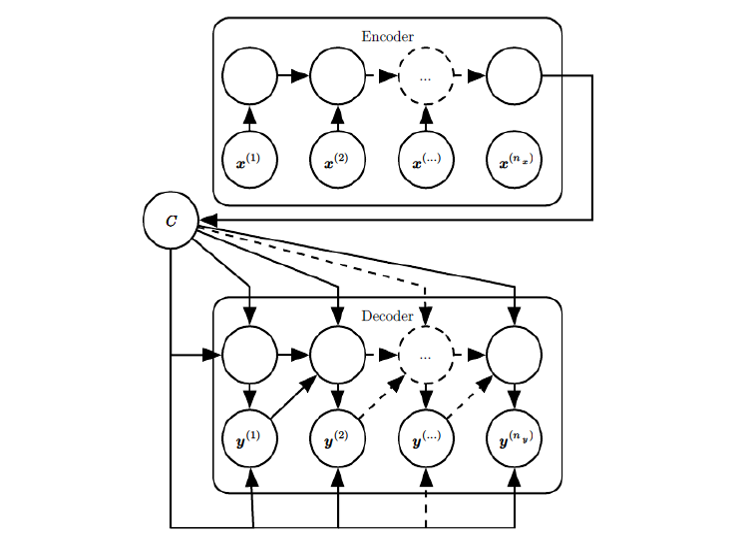
\includegraphics[width=0.8\linewidth]{images/encdec.png}
	\end{figure}
	The last state $\vh^{(n_x)}$ of the encoder RNN is typically used as a representation $\mC$ of the input sequence that is provided as input to the decoder RNN.
	One clear \textbf{limitation} of this architecture is when the context $\mC$ output by the encoder RNN has a dimension that is too small to properly summarize a long sequence.

	\subsection{Deep Recurrent Networks}
	The computation in most RNNs can be decomposed into three blocks of parameters and associated transformations\dots
	\begin{itemize}
		\item[\dots] from the input to the hidden state
		\item[\dots] from the previous hidden state to the next hidden state
		\item[\dots] from the hidden state to the output
	\end{itemize}

	\textbf{Introducing depth} can be done by many ways:
	\begin{figure}[H]
		\centering
		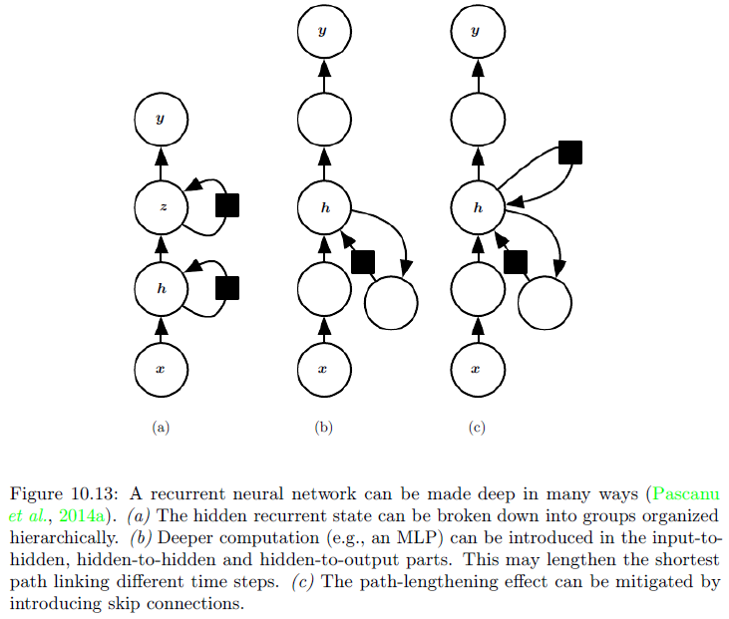
\includegraphics[width=0.9\linewidth]{images/rnn.png}
	\end{figure}

	\subsection{The Challenge of Long-Term Dependencies}
	The basic problem is that gradients propagated over many stages tend to either vanish or explode.
	Even if we assume that the parameters are such that the RNN is stable (can store memories, gradients not exploding), the difficulty with long-term dependencies arises from the exponentially smaller weights given to long-term interactions (involving the multiplication of many Jacobians) compared to short-term ones.\\
	RNNs involve the composition of the same function multiple times, once per time step.
	These compositions can result in extremely nonlinear behavior, as illustrated in the figure below.
	\begin{figure}[H]
		\centering
		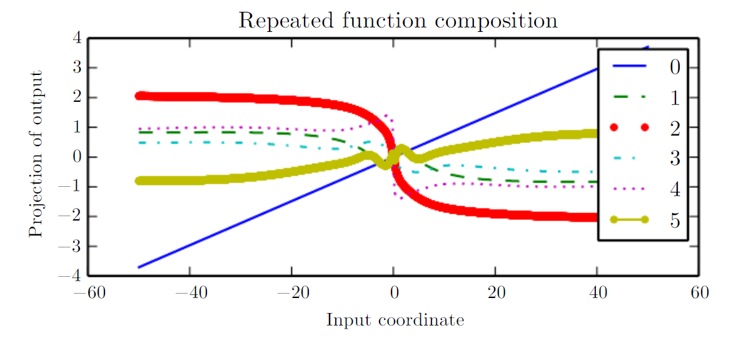
\includegraphics[width=0.9\linewidth]{images/unstable.png}
	\end{figure}
	The function composition employed by RNNs somewhat resembles matrix multiplication.
	We can think of the recurrence relationship as a simple RNN lacking a nonlinear activation function and lacking inputs:
	\[ \vh^{(t)} = \mW^T\vh^{(t-1)} \]
	This relationship can be simplified to
	\[ \vh^{(t)} = (\mW^t)^T \vh^{(0)} \]
	The eigenvalues are raised to the power of $t$ causing eigenvalues with magnitude less than one to decay to zero, and eigenvalues with magnitude greater than one to explode.
	Any component of $\vh^{(0)}$ that is not aligned with the largest eigenvector will eventually be discarded.\\

	If we make a non-recurrent network that has a different weight $w^{(t)}$ at each time step, and the initial state is given by 1, then the state at time $n$ is given by
	\[ \prod_{t=1}^{n}w^{(t)} \]

	Suppose that the $w^{(t)}$ values are generated randomly, independently from one another, with zero mean and variance:
	\begin{itemize}
		\item For independent random variables the following holds:
		\[ \var(XY) = \var(X)\var(Y)+\var(X)\Exp(Y)^2+\var(Y)\Exp(X)^2 \]
		\item Since the means are assumed to be zero, this implies that the variance of the product is the product of the variances
		\item The variance of the product is now $O(v^n)$
	\end{itemize}

	\subsection{The Long Short-Term Memory RNNs}
	The most effective sequence models used in practical applications are called \textbf{gated RNNs}.
	These include the long short-term memory \textbf{LSTM} and networks based on the gated recurrent unit \textbf{GRU}.
	These units allow the network to accumulate information over a long duration, without their derivatives vanishing or exploding.\\

	Introducing self-loops to produce paths where the gradient can flow for long durations is a core contribution of the initial LSTM model.
	A crucial addition has been to make the weight on this self-loop conditioned on the context, rather than fixed.
	By making the weight of this self-loop \textbf{gated} (controlled by another hidden unit), the time scale of integration can be changed dynamically.\\

	Instead of a unit that simply applies an element-wise nonlinearity to the affine transformation of inputs and recurrent units, LSTM RNN have \emph{LSTM cells} that have an internal recurrence (a self-loop), in addition to the outer recurrence of the RNN.
	Each cell has the same inputs and outputs as an ordinary recurrent network, but has more parameters and a system of gating units that controls the flow of information.
\end{multicols}
\begin{figure}[H]
	\centering
	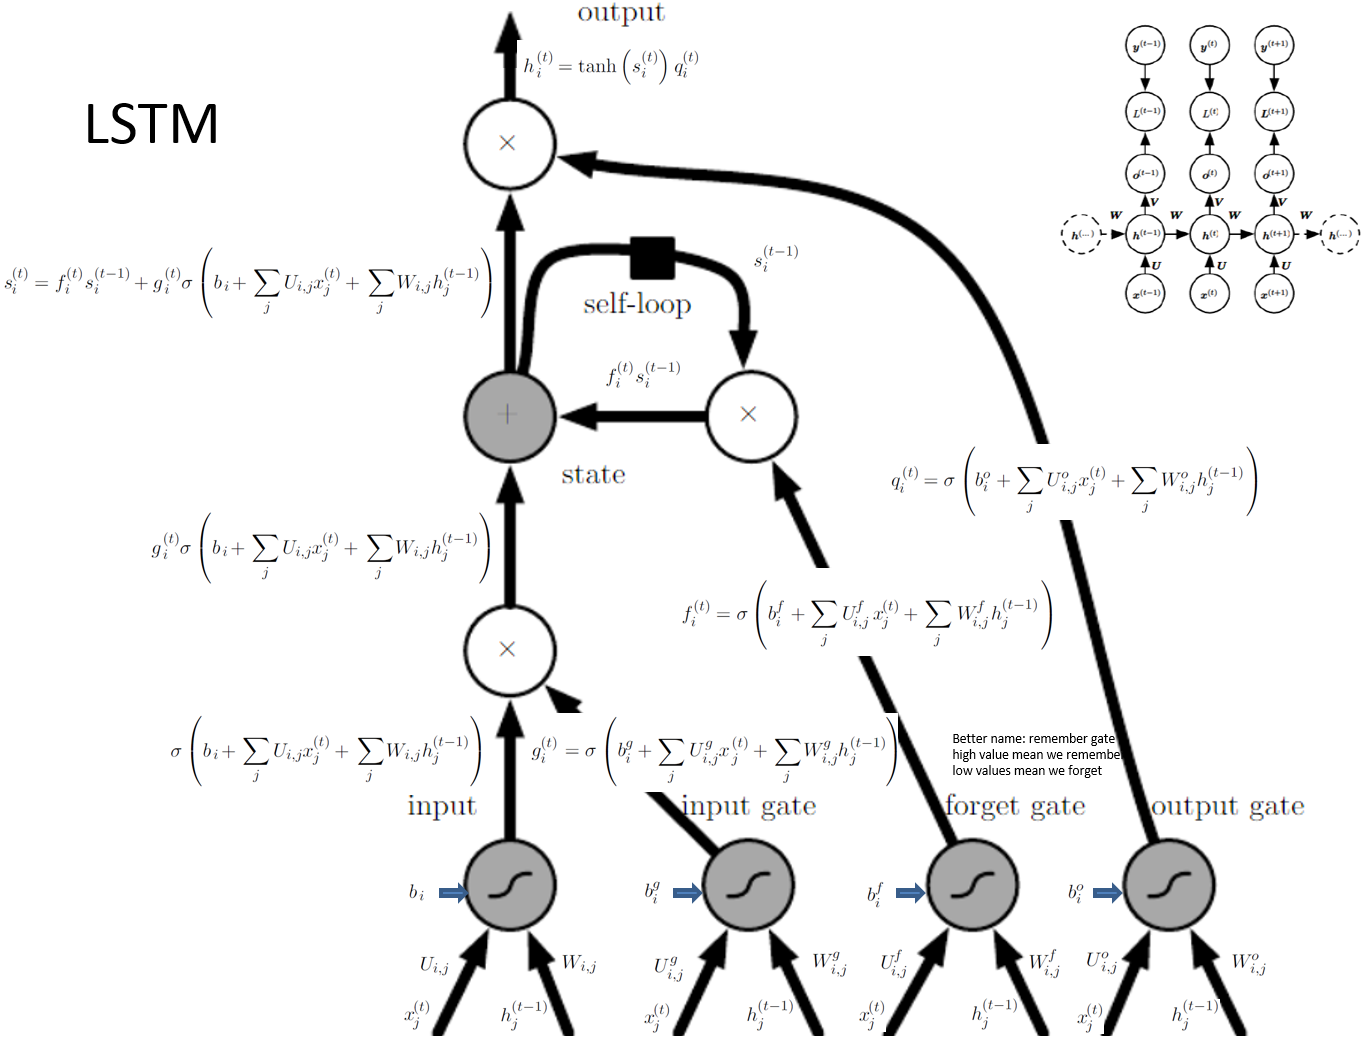
\includegraphics[width=\linewidth]{images/lstm.PNG}
\end{figure}
LSTM networks have been found extremely successful in many applications:
\begin{itemize}
	\item Unconstrained handwriting recognition
	\item Speech recognition
	\item Handwriting generation
	\item Machine translation
	\item Image captioning and parsing
\end{itemize}
\begin{figure}[H]
	\centering
	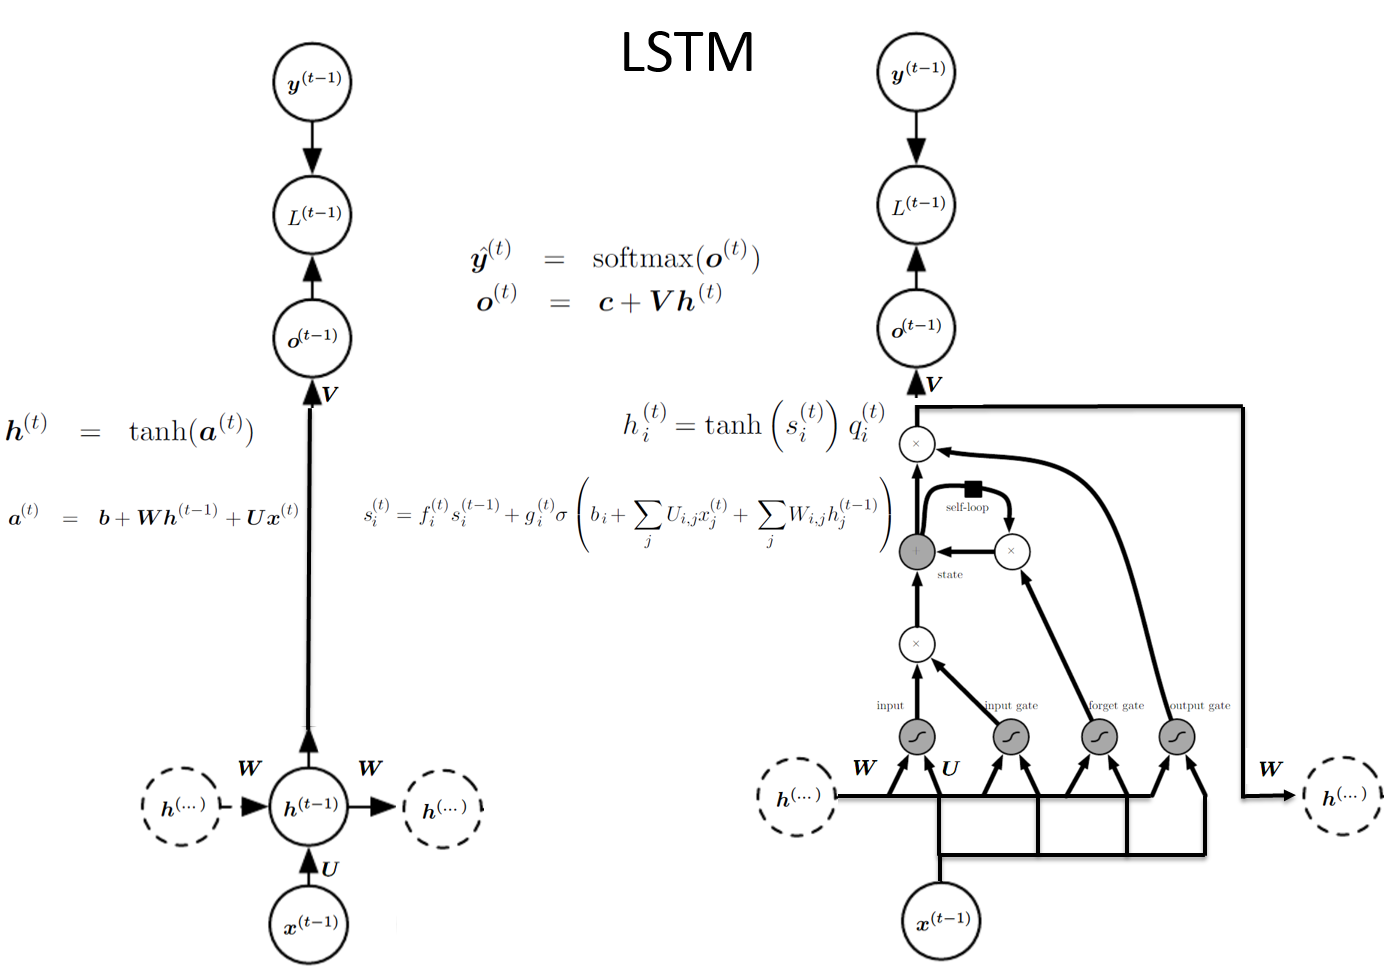
\includegraphics[width=0.9\linewidth]{images/lstm2.PNG}
\end{figure}
\begin{multicols}{2}
	\subsection{Other Gated RNNs}
	Which pieces of the LSTM architecture are necessary?
	Some answers to these questions are given by the work on gated RNNs, whose units are also known as gated recurrent units (\textbf{GRU}).
	The main difference with the LSTM is that a single gating unit simultaneously controls the forgetting factor and the decision to update the state unit.\\

	The update gates $u_i^{(t)}$ and reset gates $r_i^{(t)}$ can individually \emph{ignore} parts of the state vector.
	\begin{align*}
	u_i^{(t)} =& \sigma\left( b_i^u+\sum_j U_{i,j}^ux_j^{(t)}+\sum_j W_{i,j}^uh_j^{(t)} \right)\\
	r_i^{(t)} =& \sigma\left( b_i^r+\sum_j U_{i,j}^rx_j^{(t)}+\sum_j W_{i,j}^rh_j^{(t)} \right)\\
	h_i^{(t)} =& u_i^{(t-1)}h_i^{(t-1)} +(1-u_i^{(t-1)}) \\
	&\tanh \left( b_i+\sum_j U_{i,j}x_j^{(t-1)}+\sum_j W_{i,j}r_j^{(t-1)}h_j^{(t-1)} \right)\\
	\end{align*}
	\columnbreak
  For $h_i^{(t)}$, the book uses a $\sigma$ function instead of a $\tanh$, but it is more common to use a $\tanh$ function.
	The update gates act like conditional leaky integrators that can linearly gate any dimension, thus choosing to copy it (at one extreme of the sigmoid) or completely ignore it (at the other extreme) by replacing it by the new \emph{target state} value (towards which the leaky integrator wants to converge).
	The reset gates control which parts of the state get used to compute the next target state, introducing an additional nonlinear effect in the relationship between past state and future state.
	\begin{figure}[H]
		\centering
		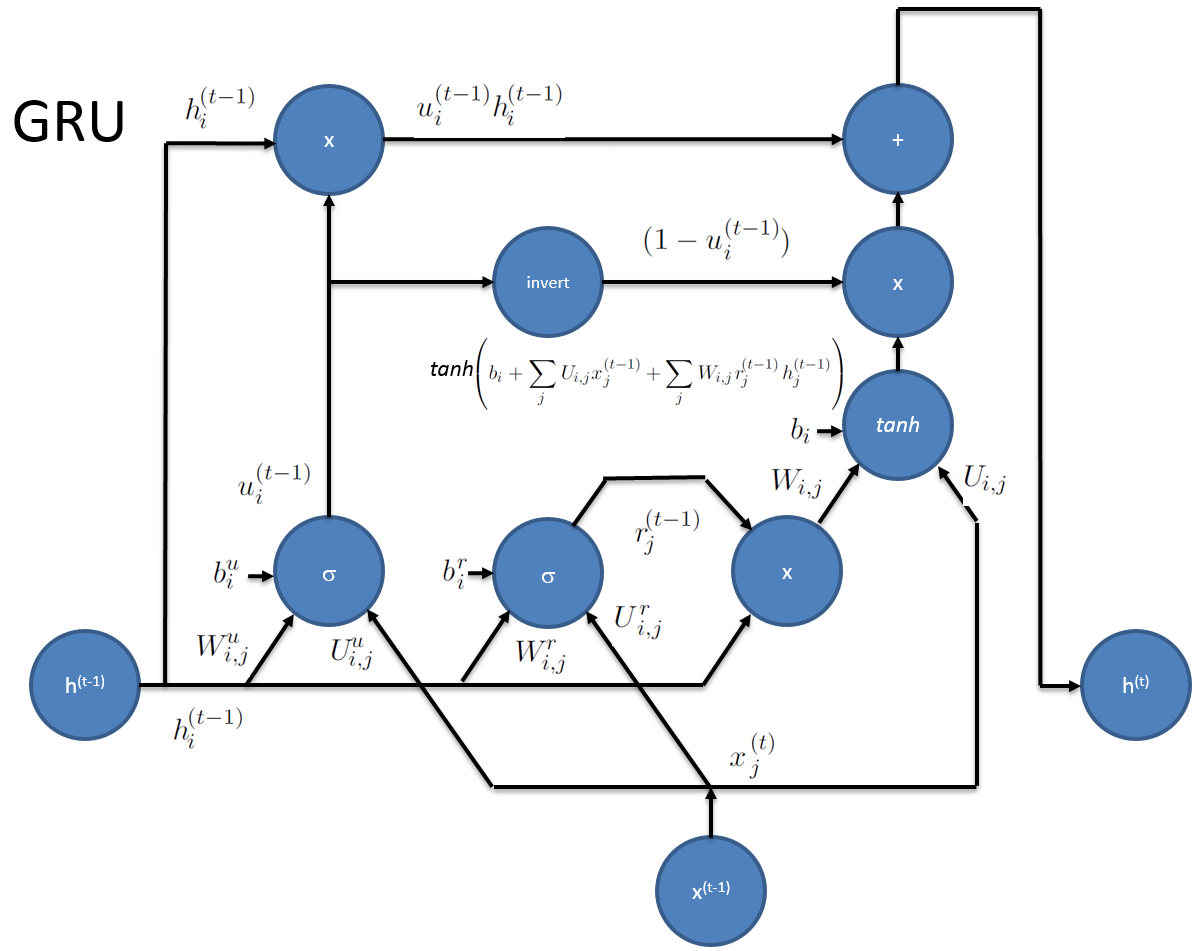
\includegraphics[width=1.05\linewidth]{images/gru.PNG}
	\end{figure}

\end{multicols}
\newpage

\section{Practical Methology}
\begin{multicols}{2}
	\subsection{Performance Metrics}
	\begin{align*}
	\text{Precision} &= \frac{t_p}{t_p+f_p} & \text{Recall} &= \frac{t_p}{t_p+f_n}\\
	\text{Specificity} &= \frac{t_n}{t_n+f_p} & \text{Accuracy} &= \frac{t_p+t_n}{t_p+t_n+f_p+f_n}\\
	\end{align*}
	\begin{itemize}
		\item Recall is also called \textbf{sensitivity}
		\item Specificity is also called \textbf{True negative rate}
	\end{itemize}
	Clearly there is a trade-off between precision and recall so a PR Curve is plotted to show this trade-off:
	\begin{figure}[H]
		\centering
		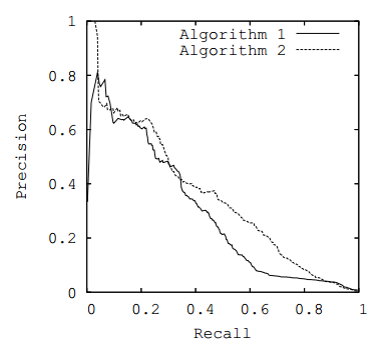
\includegraphics[width=0.75\linewidth]{images/pr_curve.png}
	\end{figure}
	If a curve is too much information, often the area under the curve is reported or alternatively the \textbf{F-score}:
	\[ F = \frac{2pr}{p+r} \]
	The fraction of examples for which the machine can make a confident decision is called the \textbf{coverage}.
	This is again a trade-off, the lower the coverage, the better the accuracy, since the machine only classifies the easy examples.\\
	
	To determine whether the training data is good enough, we can train the model until it's overfitted. The performance on the training set should be almost arbitrarily good.
	
	 
	\subsection{Selecting Hyperparameters}
	Properly selected hyperparameters often make the difference between a well working scheme and a failed scheme.
	Basically one can find these hyperparameters by hand using experience or one can use an automated approach using experiments.
	This requires insight into the effect a hyperparameter has. 
	The \textbf{table} shows some popular hyperparameters and their influence on the effective capacity.

	\subsection{Automatic Hyperparameter Optimization Algorithms}
	In principal, it should be possible to automatically find a good set of hyperparameters which results in acceptable generalization error.
	These tuning schemes have on their own new hyperparameters, but they tend to be less sensitive.\\
	
	\textbf{Grid Search: }If there are only a few parameters, a grid search is reasonable.
	For each hyperparameter a finite set of values needs to be defined, which should be explored.
	Then every possible combination of theses settings is evaluated and the setting resulting in the lowest test error is selected.
	
	\textbf{Random Search} is the preferred way of finding a good set of hyperparameters that converges much faster.
	The basic idea is, that for each hyperparameter a value is picked randomly.
	Now the test error for this random hyperparameter vector is calculated and the best vector is stored.
	
	\begin{figure}[H]
		\centering
		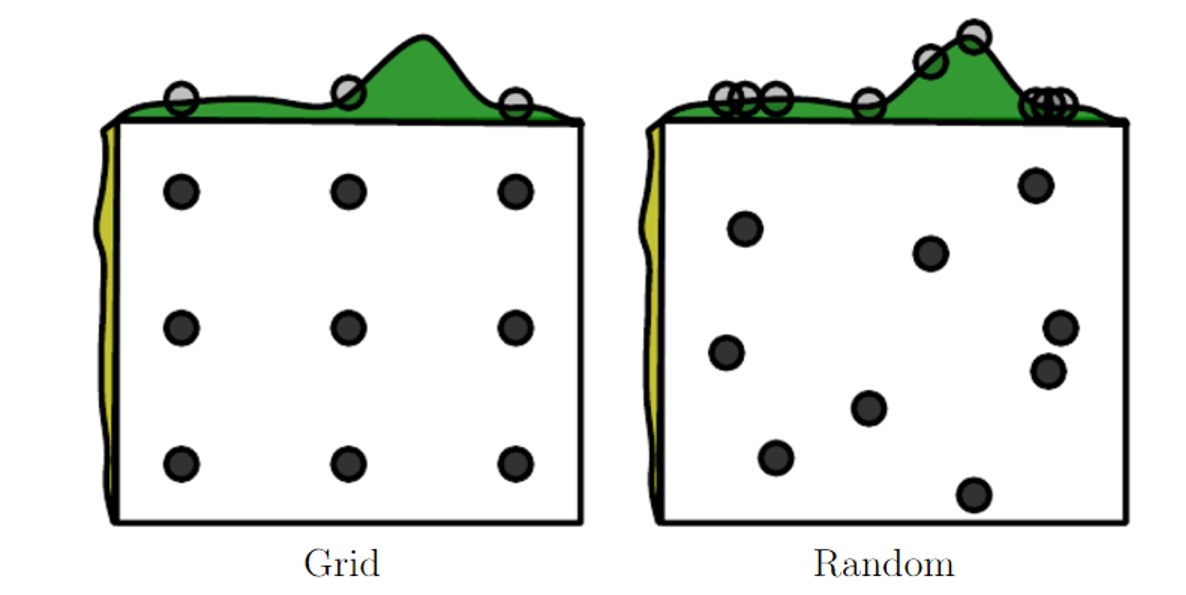
\includegraphics[width=0.75\linewidth]{images/gridrandom.PNG}
	\end{figure}
	
	\begin{figure}[H]
		\centering
		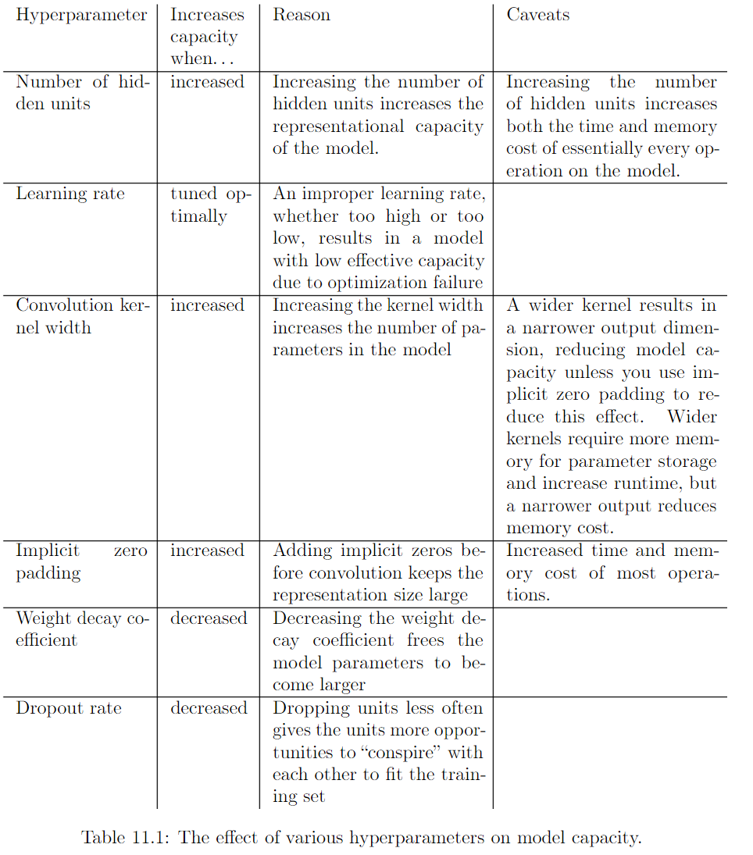
\includegraphics[width=1\linewidth]{images/hypertable.png}
	\end{figure}
	
\end{multicols}




































\section{Statistical Machine Learning}
\subsection{Statistical Learning}
\subsubsection{What is Statistical Learning?}
\begin{onehalfspace}
	\begin{tabularx}{\textwidth}{p{3cm}X}
		MSE & Mean of the squared error between the true value of the output variable and its predicted value:
		\[ E(Y-\hat{Y})^2 = E\lbrack f(X)+\epsilon -\hat{f} (X)\rbrack ^2 = \underbrace{\lbrack f(X) -\hat{f} (X)\rbrack
			^2}_\text{Reducible} + \underbrace{Var(\epsilon ) }_\text{Irreducible} \] \\
		Inference &  Relationship between the input variables (predictors) and the resulting output variable (response).
		Often $\beta$ is used:
		\[ f(X) = \beta_0 + \beta_1 X_1 + \beta_2 X_2 + ... + \beta_p X_p \] \\
		OLS & The scheme called ordinary least squares can be used to find the parameters which results in a function $f$ that fits the training data: \( Y \approx{} f(X) \) \\
		Regression & If the response variable $Y$ is is numerical, we have a regression problem \\
		Classification & If the response variable $Y$ is categorical, we have a classification problem \\
		Quantitative & Numerical variables i.e. Temperature in degree, velocity in m/s, etc... \\
		Qualitative & Categorical variable i.e. Gender (male/female), education level (B.S./M.S./PhD), etc... \\
	\end{tabularx}
\end{onehalfspace}


\subsubsection{Assessing Model Accuracy}
\begin{onehalfspace}
	\begin{tabularx}{\textwidth}{p{3cm}X}
		Measuring prediction performance & One popular measure is the MSE. Since the MSE is calculated using the training data, this is really the training MSE \[ MSE = \frac{1}{n} \sum_{i=1}^{n} (y_i-\hat{f} (x_i))^2 \]
		Low training MSE does NOT imply low testing MSE! \\
		Bias vs. Variance & The variance refers to the amount by which the estimate of $f$ would change if we estimated it using a different training set whereas the bias refers to the error introduced by approximating a real-life	problem by a model
		\[ E(y_0 -\hat{f}(x_0))^2 = Var(\hat{f}(x_0)) + \lbrack Bias(\hat{f}(x_0))\rbrack ^2 +Var(\epsilon ) \]
		\[ Bias(\hat{f}(x_0)) = E\lbrack f(x_0)-\hat{f}(x_0)\rbrack \] \\
		Classification error & The quality of the estimated function $f$ can not be measured using MSE since the output $Y$ is categorical. Therefore the following definition of a training error rate is used:
		\[ \frac{1}{n} \sum_{i=1}^{n} I(y_i\neq \hat{y}_i) \] \\
		KNN & The K-nearest neighbors is used for classification problems. As the name suggests, the K-nearest data points	"vote"{} to which class a new point belongs. \\
	\end{tabularx}
\end{onehalfspace}

\subsection{Linear Regression}
\subsubsection{Simple Linear Regression}
\begin{onehalfspace}
	\begin{tabularx}{\textwidth}{p{3cm}X}
		Estimating coefficients & In practice the coefficients are unknown and need to be learned (estimated) from the n training data sets \( (x_1,y_1), (x_2,y_2),..., (x_n,y_n) \). The goal of the estimation process is, that the two parameters are found such that each training data set is estimated as close as possible:
		\( \hat{y}_i = \hat{\beta}_0+\hat{\beta}_1 x_i \) \\
		Residuals & The residuals are defined as the difference between the measured and the estimated output value:
		\( e_i = y_i-\hat{y}_i \) \\
		RSS & The residual sum of squares is one approach to define the closeness of the coefficients to the real values. It	is defined as \( RSS = e^2_1+e^2_2+...+e^2_n = \mysum (y_i-\hat{y}_i)^2\)
		Good models result in a small RSS. \\
		TSS & The total sum of squares is $n$ times the sample variance of the residual $(y-\hat{y})$:
		\[ RSS=\mysum (y_i-\hat{y}_i)^2 \] TSS only depends on the data, not on the model.
		The expression $\frac{TSS-RSS}{p}$ calculates the improvement by the model per parameter $p$ for all samples $n$. \\
		Sample Mean & \[ \bar{x} \equiv{} \frac{1}{n} \sum_{i=1}^{n} x_i  \qquad
		\bar{y} \equiv{} \frac{1}{n} \sum_{i=1}^{n} y_i \] \\
		Least Squares & The least squares approach selects the two parameters such, that the RSS is minimized:
		\[ \hat{\beta}_1 = \frac{\sum_{i=1}^{n} (x_i-\bar{x})(y_i-\bar{y})}{\sum_{i=1}^{n} (x_i-\bar{x})^2}  \qquad
		\hat{\beta}_0 = \bar{y}-\hat{\beta}_1 \bar{x} \] \\
	\end{tabularx}
\end{onehalfspace}

\subsubsection{Assessing the Accuracy of the Coefficient estimates}
\begin{onehalfspace}
	\begin{tabularx}{\textwidth}{p{3cm}X}
		Accuracy & If the relationship $Y = f(X)+\epsilon$, where the function $f$ is unknown and the error $\epsilon$ is	random with mean zero, is assumed to be true, then it can be written as $Y = \beta_0+\beta_1 X+\epsilon$ \\
		SE & The standard error tells us the average amount this estimate differs from the true value
		\[ SE(\hat{\mu})^2 = Var(\hat{\mu}) = \frac{\sigma^2}{n} \qquad \sigma^2 = Var(\epsilon) \]
		The following formulas are approximations which assume that the errors for each observation are uncorrelated with	the common variance, which is not strictly true. Nevertheless, these formulas show that these estimators are	consistent:
		\[ SE(\hat{\beta}_0)^2 = \sigma^2 \left[ \frac{1}{n}+\frac{\bar{x}^2}{\sum_{i=1}^{n}(x_i-\bar{x})^2} \right] \qquad
		SE(\hat{\beta}_1)^2 = \frac{\sigma^2}{\mysum (x_i-\bar{x})^2}  \] \\
		Null Hypothesis & The most common hypothesis test involves testing the null hypothesis versus the alternative	hypothesis: \[ H_0 : \beta_1 = 0 \rightarrow \text{There is no relationship between } X \text{ and } Y \]
		\[ H_a : \beta_1 \neq 0 \rightarrow \text{There is some relationship between } X \text{ and } Y \]
		If there is no relationship, we would expect the slope to be zero. Since the slope is never really exactly zero, we need to measure how far away the slope is from zero\\
	\end{tabularx}

	\begin{tabularx}{\textwidth}{p{3cm}X}
		t-Statistics & The solution to test the null hypothesis is to express the estimate of the slope in multiples of the	standard error, calculating the so called t-statistics: \[ t = \frac{\hat{\beta}_1 - 0}{SE(\hat{\beta}_1)} \]
		If there is no relationship between $X$ and $Y$ then the random variable $t$ should have a t-distribution with	$n-2$ degrees of freedom. For $n>30$ the t-distribution is very similar to a normal (Gaussian) distribution\\
		$R^2$-Statistics & The $R^2$-Statistics is the proportion of the variance explained by the model and hence it takes values between $0$ and $1$. This makes it independent of the units of $Y$. It measures the proportion of variability in $Y$ that can be explained using $X$:
		\[ R^2=\frac{TSS-RSS}{TSS}=1-\frac{RSS}{TSS}=1-\frac{\mysum (y_i-\hat{y}_i)^2}{\mysum (y_i-\bar{y})^2} \]
		For simple linear regression the $R^2$-Statistic is identical to the sample correlation squared:
		\[ Cor(X,Y)=\frac{\mysum (x_i-\bar{x})(y_i-\bar{y})}{\sqrt{\mysum (x_i-\bar{x})^2}\sqrt{\mysum (y_i-\bar{y})^2}} \]
		\\
		F-Statistics & F expresses the improvement of the model per parameter $p$ in multiples of the residual variance:
		\[ F=\frac{(TSS-RSS)/p}{RSS/(n-p-1)} \]
		If this is larger than 1, the model is working well.
	\end{tabularx}
\end{onehalfspace}

\subsubsection{Multiple Linear Regression}
In general, the multiple linear regression model takes on the following form,
each predictor variable gets its own slope and there is a common intercept:
\[ Y=\beta_0+\beta_1X_1+\beta_2X_2+...+\beta_pX_p+\epsilon \]
One interpretation of a particular slope $\beta_j$ is, that it captures the average effect on $Y$ of one unit increase in $X_j$, holding all other predictors fixed. Just as in the simple regression case, the coefficients (parameters) are estimated in such a way, that the sum of squared residuals in the training data is minimized:
\[ RSS=\mysum(y_i-\bar{y}_i)^2=\mysum(y_i-\hat{\beta}_0-\hat{\beta}_1x_{i1}-\hat{\beta}_2x_{i2}-...-\hat{\beta}_px_{ip})^2 \]



\subsection{Classification}
\subsubsection{An Overview of Classification}
Why not linear regression for qualitative responses? $\rightarrow$ Because  coding  responses  implies  an order  and  a  distance, i.e.
\[ Y = \begin{cases}
1\texttt{ if stroke} \\ 2\texttt{ if drug overdose} \\ 3\texttt{ if epileptic seizure}
\end{cases}  \]
Now the coding created an  order and also implies that  selecting  stroke,  if  it  is  really  a drug  overdose  is  equally  bad  as  selecting epileptic  seizure,  if  it  is  really  a  drug overdose \\

\subsubsection{Logistic Regression}
Instead of modeling the response, logistic regression models the probability that the response belongs to a particular category.
Hence the idea is to use the logistics function, which goes in an S-shape smoothly from 0 to 1 and model  its argument using a linear model:
\[ p(X) = \frac{e^{\beta_0+\beta_1X}}{1+e^{\beta_0+\beta_1X}}  \]
With some manipulation the following equation results, where the term on the left hand side is called the  odds:
\[ \frac{p(X)}{1-p(X)} = e^{\beta_0+\beta_1X} \qquad \rightarrow \qquad \log \left( \frac{p(X)}{1-p(X)} \right) = \beta_0+\beta_1X\]

\subsubsection{Estimating the Regression Coefficients}
\paragraph*{The basic approach}for finding the unknown coefficients given the training data is called the maximum likelihood approach.
The goal is to pick the coefficients in such a way, that the probability of the model having created the observed data is maximized.
\[ \ell (\beta_0,\beta_1) = \prod_{i:y_i=1} p(x_i) \prod_{i':y_{i'}=1} (1 - p(x_{i'})) \]
If we assume that all training data is statistically independent, then the total probability is simply  the product of all the default cases and the non-default cases.
The coefficient estimates are now selected such that the likelihood function (in this case the probability) is maximized.
While the detail of the optimization is out of the scope for this class, any statistical software can do  that. The following table shows the resulting coefficients for the Default data set:  \\
\begin{center}
	\begin{tabular}{l|r r r r}
		& Coefficient & Std. Error & Z-Statistics & P-Value \\
		\hline
		\texttt{Intercept} & -10.6513 & 0.3612 & -29.5 & < 0.0001 \\
		\texttt{balance} & 0.0055 & 0.0002 & 24.9 & < 0.0001 \\
	\end{tabular}
\end{center}
The Z-Statistic plays the role of the t-Statistic  and is defined as $\hat{\beta}_1/SE(\hat{\beta}_1)$.
High absolute values indicate evidence against the null hypothesis $H_0 : \beta_1=0$. \\

\subsubsection{Linear Discriminant Analysis}
As we have just seen, we need to know the probability of a class, given some observations, to make the optimal class decision.
In linear discriminant analysis (LDA) we go the other way around, we estimate the probability density functions of the observations $X$, given a particular class $Y$, i.e. $p(X|Y)$.
Then we apply Bayes theorem to flip these probabilities around and get the one on the right, which allow us to make an optimal decision:
\[ P(Y|X)=\frac{P(X|Y)P(Y)}{P(X)} \]

{\renewcommand{\arraystretch}{1.5}
	\subsubsection{Using Bayes' theorem for classification}
	We want to classify observations into K classes. We need to know what the probability of each class is, without having any observation.
	This is called the prior probability $\pi_k$. We need to know what the pdf's for each of the observations, given a particular class k.
	This is the likelihood of an observation, given a particular class $f_k(X)=p(X|Y=k)$.
	\begin{itemize}
		\item $f_k(x)$ is relatively large, if there is a high probability that an observation in the k\ts{th} class has a value around a small neighborhood of $x$
		\item $f_k(x)$ is relatively small, if there is a low probability that an observation in the k\ts{th} class has a value around a small neighborhood of $x$
		\item Note that the integral over the small neighborhood is actually the probability
	\end{itemize}
	Bayes' theorem states \[ Pr(Y=k|X=x)=\frac{\pi_kf_k(x)}{\sum_{l=1}^{K}\pi_lf_l(x)}\]
	To keep the notation light and consistent with the previous chapters, the following abbreviation is used:
	\[ p_k(X)=Pr(Y=k|X)\]
	Note that this is called the posterior probability that an observation $X$ belongs to class k.
	Selecting the class which has the largest posterior probability results in the lowest average number of errors. \\
	Here's a simple example with two classes $A$ and $B$ and continuous observations X: \\
	\\
	$P(Y|X)=\frac{P(X|Y)P(Y)}{P(X)}$ where $P(X)=P(X|Y=A)P(Y=A)+P(X|Y=B)P(Y=B)$ hence
	\[ P(Y=A|X)=\frac{P(X|Y=A)P(Y=A)}{P(X|Y=A)(P(Y=A)+P(X|Y=B)P(Y=B))} \text{ and } \]
	\[ P(Y=B|X)=\frac{P(X|Y=B)P(Y=B)}{P(X|Y=A)(P(Y=A)+P(X|Y=B)P(Y=B))} \]
	pick the class $A$ or $B$ that has a higher probability given the measured data $X$. \\
	Bayes' theorem suggests, that instead of modeling $p_k(X)$ directly (as is done with logistic regression) one could model/estimate $f_k(x)$ and $\pi_k$ and then use the theorem to find the needed $p_k(X)$
	\[ Pr(Y=k|X=x)=\frac{\pi_kf_k(x)}{\sum_{l=1}^{K}\pi_lf_l(x)} \]
	Estimating the prior probabilities $\pi_k$ is easy, simply use the fraction of samples in the training set that belong to class k as the estimate of the prior probabilities.
	Without any observations, that is clearly the best possible guess.
	Estimating $f_k(X)$ is more challenging, except we assume some parametric form.
	Hence being able to estimate $f_k(X)$ will allow us to use Bayes' theorem to calculate the posterior probabilities
	for each class and selecting the class with the highest posterior probability will result in the smallest error rate.


\subsection{Resampling Methods}
\subsubsection{Introduction}
As the name implies, these are methods which use the given training set over and over again.
This is achieved by sampling that set, i.e., create different subsets.
To each of these subsets, the model can be fitted which allows for a statistical evaluation of the fitting.
The focus will be on two fundamental resampling methods, Cross-validation and Bootstrap.

\subsubsection{Cross-Validation}
Cross-validation can be used to estimate the test error in order to evaluate the performance of a method and finding an optimal flexibility  setting.
The training error rate is the average error that results when the training data is evaluated with the trained model (note that the model has seen all the samples in the training set and hence, this rate must be low for a reasonable  system).
The test error rate is the average error that results when predicting the response to a NEW observation.
Since the model has never seen these samples, the test error rate is the rate we would like to minimize.
Usually the training error rate is smaller than the test  error rate.
If the training error rate is a lot smaller, that implies that the system is overtrained.
If we have a large test data set, then calculating the test error rate is simple, but that is almost never the case.
Since no test set is available, the basic idea is to hold out some samples from the training set and then use these as test set.
There are different approaches to do this.

\subsubsection{Cross-Validation: The Validation Set Approach}
The Validation Set Approach is the most basic approach of cross-validation.
The given observations are randomly split into two equally sized sets, a training set and a validation set (hold-out set).
The model is then trained using the training set and after that the model is tested using the validation set.

\begin{itemize}
	\item For a quantitative response, the validation MSE can be calculated (an estimate of the test MSE)
	\item For a qualitative response, the validation error rate can be calculated (an estimate of the test error rate)
\end{itemize}

The validation set approach is conceptually simple and easy to implement, but there are two potential problems:

\begin{itemize}
	\item The validation MSE (an estimate of test MSE) can vary by a large amount since it depends on which observations are in the training set and which observations are in the validation sets
	\item Since only a subset of the observations is used to train the model, the resulting model is probably not as good as it could be. Hence the validation MSE probably overestimates the test MSE if the entire training set could have been used for training the model
\end{itemize}

\subsubsection{Cross-Validation: Leave-One-Out}
Like the previous approach, Leave-One-Out Cross-Validation (LOOCV) splits the observations into two parts.
The difference is that now the validation set only uses one single observation.
This means that now the model can be fitted to almost all the data ($n-1$) and then the prediction is made for the one single sample that was left out.
Hence the MSE of this single sample is an approximately unbiased estimate of the test MSE.
\begin{itemize}
	\item Even if it's unbiased, it's a poor estimate since it has a high variance.
	\item This variance can be reduced by repeating the procedure by systematically leaving out one sample after the other and then averaging the resulting single sample MSEs
\end{itemize}
The main advantages over the validation set approach are:
\begin{itemize}
	\item ($n-1$) data points are used to fit the model instead of $n/2$ hence there is almost no bias
	\item No randomness in the procedure (Running LOOCV twice will result in the identical values for the estimated test MSE)
\end{itemize}

LOOCV is computationally quite expensive since the model has to be fitted $n$ times $\rightarrow$ Usually $n$ is large which results in a slow model fitting.
Anyhow, there is one great exception for least squares linear (or polynomial) regression.
The following formula can be used to calculate the estimated test MSE using the LOOCV approach:
\[ CV_{(n)}=\frac{1}{n} \mysum \left( \frac{y_i-\hat{y}_i}{1-h_i} \right)^2 \qquad \text{with} \qquad
h_i= \frac{1}{n}+ \frac{(x_i-\bar{x})^2}{\sum_{i'=1}^{n}(x_{i'}-\bar{x})^2} \]
What makes this formula powerful is the fact that the model needs to be fitted only once to all the data.
Then in the calculation of the training MSE, each term needs to be scaled by $1/(1-h_i)$ where $h_i$ is the leverage of the $i^{th}$ training sample.
Recall the leverage lies between $1/n$ and 1 and measures how strongly an observation influences its own fit.
Hence the residuals for high leverage points are scaled up by exactly the right amount so that the equation is true.

\subsubsection{Bootstrap}
Most commonly used to provide a measure of accuracy of a parameter estimate and/or of a given statistical learning method and the uncertainty associated with a given estimator.
Example: Investing a fixed sum of money into two financial assets with returns of X and Y (both variables are random):
\[ Var(\alpha X+(1-\alpha)Y) \qquad \alpha =\frac{\sigma_Y^2-\sigma_{XY}}{\sigma_X^2+\sigma_Y^2-2\sigma_{XY}}\]
X and Y are correlated and the goal is to minimize the variance (risk proxy) of the overall investment.
In reality, the variance and the covariance is not known and need to be estimated using a data set that contains past measurements of X and Y.
Now we can estimate a value for $\alpha$ that will minimize the variance of the investment.

\subsection{Abbreviations}
{\renewcommand{\arraystretch}{2}
	\begin{tabular}{l p{5cm} l}
		\textbf{Abb.} & \textbf{Meaning} & \textbf{Formula}  \\
		$MSE$ & Mean Squared Error & $ MSE=\frac{1}{n}\mysum (y_i-\hat{f}(x_i)) $ \\
		$RSS$ & Residual Sum of Squares & $RSS= \mysum (y_i-\hat{y}_i)^2 = e_1^2+e_2^2+...+e_n^2$ \\
		$TSS$ & Total Sum of Squares & $TSS=\mysum (y_i-\bar{y})^2$ \\
		$SE$ & Standard Error &
		$ SE(\hat{\beta}_0)^2 = \sigma^2 \left[ \frac{1}{n}+\frac{\bar{x}^2}{\sum_{i=1}^{n}(x_i-\bar{x})^2} \right] \qquad SE(\hat{\beta}_1)^2 = \frac{\sigma^2}{\mysum (x_i-\bar{x})^2}$ \\
		$RSE$ & Residual Standard Error & $RSE=\sqrt{\frac{1}{n-2}RSS}=\sqrt{\frac{1}{n-2}\mysum (y_i-\hat{y}_i)^2}$ \\
		$R^2$ & R-Statistics & $R^2=\frac{TSS-RSS}{TSS}=1-\frac{RSS}{TSS}$ \\
		$F$ & F-Statistics & $F=\frac{(TSS-RSS)/p}{RSS/(n-p-1)}$ \\
		$h_i$ & Leverage Statistics & $h_i=\frac{1}{n}+\frac{(x_i-\bar{x})^2}{\sum_{i'=1}^{n}(x_{i'}-\bar{x})^2}$ \\
		$VIF$ & Variance Inflation Factor & $VIF(\hat{\beta}_j)=\frac{1}{1-R^2_{X_j|X_{-j}}}$ \\
		$\ell(\beta_0,\beta_1)$ & Likelihood Function &
		$\ell (\beta_0,\beta_1) = \prod_{i:y_i=1}p(x_i) \prod_{i':y_{i'}=1} (1 - p(x_{i'}))$ \\
		$f_k(X)$ & PDF for each Observation \newline given particular class k &
		$f_k(X)=p(X|Y=k)$ \\
		$\pi_k$ & Prior Probability & $\pi_k=Pr(Y=k)$\\
		$p_k(X)$ & Posterior Probability & $p_k(X)=Pr(Y=k|X)$ \\
		$LDA$ & Linear Discriminant Analysis & $f_k(x)=\frac{1}{\sqrt{2\pi}\sigma_k}\exp \left(-\frac{1}{2\sigma^2_k}(x-\mu_k)^2\right)$ \\
		$CV_{(k)}$ & k-fold Cross-Validation & $CV_{(k)}= \frac{1}{k} \sum_{i=1}^{k} MSE_i$ \\
		$LOOCV$ & Leave One Out Cross-Validation & $CV_{(n)}= \frac{1}{n} \sum_{i=1}^{n} MSE_i
		=\frac{1}{n} \sum_{i=1}^{n} \left( \frac{y_i - \hat{y}_i}{1-h_i} \right)  $\\
		$h_i$ & Leverage of sample $i$ & $h_i= \frac{1}{n} $ \\
		$RR$ & Ridge Regression & $ \mysum \left( y_i-\beta_0 - \sum_{j=1}^{p} \beta_j x_{ij} \right)^2 + \lambda \sum_{j=1}^{p} \beta_j^2 = RSS + \lambda \sum_{j=1}^{p} \beta_j^2$ \\
	\end{tabular}


\end{document}
